% !TeX encoding = UTF-8
% !TeX program  = xelatex

\documentclass[12pt,a4paper,openany,
               afrikaans,UKenglish,
               masters-t,goldenblock 
              ]{stb-thesis} 
% \usepackage{parskip}
%==== Language setup =================================================
\usepackage{babel}
\usepackage[utf8]{inputenc}%...................... Unicode input file format

%==== Math setup =====================================================
\usepackage{amsmath}%............................. Advanced math (before fonts)
%\usepackage{amssymb}%............................ AMS Symbol fonts

%==== Font setup (default is Computer Modern) ========================
\usepackage{iftex}
\ifxetex
    \usepackage[math-style=TeX,
                bold-style=TeX,
               ]{unicode-math}
    \setmainfont{Cambria}%........................ Unicode fonts  (Win)                
    \setsansfont[Scale=MatchLowercase]{Calibri}
    \setmonofont[Scale=MatchLowercase]{Consolas}
    \setmathfont{Cambria Math}
    \defaultfontfeatures{Ligatures=TeX}
    \let\bm\symbfit
\else
    \usepackage[utf8]{inputenc}%.................. Unicode file format
    \usepackage{textcomp}%........................ Additional text symbols
    \usepackage[T1]{fontenc}%..................... Type 1 outline fonts
    \usepackage{bm}%.............................. Bold math fonts
\fi
\normalfont

%==== Units and numbers ==============================================
\usepackage{siunitx}%............................. Unit, number and angle output
    \sisetup{detect-all = true, detect-family = true}
    \sisetup{%output-decimal-marker = {.} ,
             group-separator = {\,},
             number-unit-product = {\,},
             inter-unit-product = \mathord{\cdot},
             exponent-product = \mathord{\times},
             separate-uncertainty = true}
   
         
%==== Ref's, Bib's and Nomencl =======================================
\usepackage{stb-nomencl}%......................... List of symbols 
    \renewcommand*{\UnitLabel}[1]{~[\,$\unit{#1}$\,]}
\usepackage{stb-bib}%............................. Bibliography (natbib internally)
    \bibliographystyle{stb-bib-eng-a}
    \renewcommand\bibfont{\small}
    \renewcommand\bibsection{\chapter{\bibname}}
\usepackage[printonlyused,withpage]{acronym}
\usepackage{hyperref}
\hypersetup{
    colorlinks,
    citecolor=black,
    filecolor=black,
    linkcolor=black,
    urlcolor=black
}
    
%==== Tables + Graphics + Color =====================================
\usepackage{array}%............................... Extended table defs 
    \setlength{\extrarowheight}{2pt}
\usepackage{longtable}%........................... Tables can break over pages
\usepackage{graphicx}%............................ Included graphics
\usepackage[font=small]{caption}%................. Customize captions  
\usepackage[table]{xcolor}%....................... Color setup + colortbl 
\usepackage{pdfpages}
\graphicspath{ {./figs} }
    
%==== Extra defs for template ========================================
\makeatletter
%---- TOC entries and case
    \addto{\captionsafrikaans}{\renewcommand\bibname{Lys van verwysings}}
    \addto{\captionsafrikaans}{\renewcommand\contentsname{Inhoudsopgawe}}
    \addto{\captionsafrikaans}{\renewcommand\listfigurename{Lys van figure}}
    \addto{\captionsafrikaans}{\renewcommand\listtablename{Lys van tabelle}}

    \addto{\captionsUKenglish}{\renewcommand{\bibname}{List of references}}
    \addto{\captionsUKenglish}{\renewcommand\contentsname{Table of contents}}
    \addto{\captionsUKenglish}{\renewcommand\listfigurename{List of figures}}
    \addto{\captionsUKenglish}{\renewcommand\listtablename{List of tables}}

%==== User Defs ======================================================
%
% Please insert user defined commands here
% and NOT in the document itself!
%

\makeatother

%==== Title Page =====================================================
\title{\bfseries
       \AorE{%-- Afrikaans ------------------------------------------
             Diskrete Element Modellering van 'n Vibrerende Skeurploeg\\[1ex]
             \normalfont\small\itshape
             (``Discrete Element Modeling of a Vibratory Subsoiler'')
            }{%-- English -------------------------------------------
             Motion Control of a Hexapod Robot Over Uneven Terrain Using Signed Distance Fields}}

\author{A.P.\ Lotriet}{Andries Phillipus Lotriet}

\degree{\AorE{MIng (Meg)}{MEng (EE)}}
       {\AorE{Magister in Ingenieurswese (Elektronies)}
             {Master of Engineering (Electronic)}}

\address{\AorE{%-- Afrikaans ----------------------------------------
        Departement Meganiese en Megatroniese Ingenieurswese,\\
        Stellenbosch Universiteit,\\
        Privaatsak X1, Matieland 7602, Suid Afrika.%
             }{%-- English ------------------------------------------
        Department of Electrical and Electronic Engineering,\\
        Stellenbosch University,\\
        Private Bag X1, Matieland 7602, South Africa.}}

\faculty{\AorE{Fakulteit Ingenieurswese}%
              {Faculty of Engineering}}

\supervisor{Prof.\ J.A.A.\ Engelbrecht}
% \cosupervisor{Prof.\ J.\ Smith}

\setdate{3}{2023}

%\SetSponsor{The financial assistance of the National Research Foundation (NRF)
%    towards this research is hereby acknowledged. Opinions expressed and
%    conclusions arrived at, are those of the author and are not necessarily to
%    be attributed to the NRF.}


%==== Main Document ==================================================
\setcounter{secnumdepth}{3}
\setcounter{tocdepth}{2}
\raggedbottom
\begin{document}   

\frontmatter%---------------------------------------------------------                    
\TitlePage

\DeclarationDate{2023/02/10}
\DeclarationPage


% \begin{abstract}[english]%===================================================
\chapter*{Abstract}
In recent times great strides have been made in the field of autonomous robotics, 
especially with regards to autonomous navigation of wheeled and aerial drones.
Legged robotics however still face numerous problems before they can become practical
to use, the most egregious of these problems being balancing of the robot, and optimal foot placement.

This thesis focuses on providing a solution to the latter problem of foot placement. This is achieved by using a depth camera to, in real time, construct a localised map of the environment, and subsequently analysing  said map for optimal foot placement locations. The system is then tested using a hexapod robot, both in simulation and on a physical robot.
% \end{abstract}


\chapter*{Uittreksel}
% \begin{abstract}[afrikaans]%=================================================
    In onlangse tye is groot vordering gemaak in die gebied van outonome robotika, 
    veral met betrekking tot outonome navigasie van hommeltuie. Bebeende-robotika het egter steeds probleme om op te los voordat dit prakties gebruik kan word, die mees ernstige van hierdie probleme is balansering van die robot, en optimale voetplasing.

    Hierdie tesis fokus daarop om 'n oplossing vir die laasgenoemde probleem van voetplasing voor te stel. Dit word bereik deur 'n dieptekamera te gebruik  om 'n gelokaliseerde kaart van die omgewing te konstrueer, en daarna die kaart te ontleed vir optimale voetplasings areas. Die stelsel word dan getoets met behulp van 'n seskantige-robot, beide in simulasie en op 'n fisiese robot.
% \end{abstract}

\chapter*{Acknowledgments}
    I would like to thank my supervisor, Prof. J.A.A Engelbrecht for his invaluable support and guidance throughout the course of this project. Additionally, I would like to thank my family and friends for their support and taking a keen interest in my work.

\chapter*{Dedication}



% Use \chapter*{} before TOC
\tableofcontents
% Use \chapter{} after TOC

\listoffigures
\listoftables
\chapter{List of symbols}
% Use stb-nomenclature + siunitx

\begin{Nomencl}[1cm]
\NomGroup{Constants}%-----------------------------------------------
    \item[$L_0 = $] \qty{300}{mm}

\NomGroup{Variables}%-----------------------------------------------
    \item[$\mathit{Re}_\mathrm{\,D}$]
                       \UnitLine{Reynolds number (diameter)}{~}
    \item[$x$]         \UnitLine{Coordinate                }{m}
    \item[$\ddot{x}$]  \UnitLine{Acceleration              }{m/s^2}\\
    
    \item[$\theta$]    \UnitLine{Rotation angle            }{rad}
    \item[$\tau$]      \UnitLine{Moment                    }{\newton\meter}

\NomGroup{Vectors and Tensors}%-------------------------------------
    \item[$\overrightarrow{\bm{v}}$] Physical vector, see equation ...

\NomGroup{Subscripts}%----------------------------------------------
    \item[$\mathrm{a}$] Adiabatic
    \item[$a$]          Coordinate

\end{Nomencl}

% \begin{Nomencl}[1cm]
% \NomGroup{Abreviations}%-----------------------------------------------
    % \item[DEM] Discrete Element Method
    % \item[FEA] Finite Element Analysis
    \begin{acronym}[MMIIII]
    \NomGroup{Abreviations}%-----------------------------------------------
        \acro{ik}[IK]{Inverse Kinematics}
        \acro{sdf}[SDF]{Signed Distance Field}
        \acro{mujoco}[MuJoCo]{Multi-Joint dynamics with Contact}
        \acro{gui}[GUI]{Graphical User Interface}
        \acro{ros}[ROS]{Robot Operating System}
        \acro{lidar}[LiDAR]{Light Detection and Ranging}
        \acro{rgbd}[RGB-D]{Red Green Blue Depth}
        \acro{slam}[SLAM]{Simultaneous Localisation and Mapping}
        \acro{imu}[IMU]{Inertial Measuring Unit}
        \acro{rl}[RL]{Reinforcement Learing}
        \acro{ann}[ANN]{Artificial Neural Network}
        \acro{gps}[GPS]{Global Positioning System}
    \end{acronym}    
% \end{Nomencl}



\mainmatter%----------------------------------------------------------
\numberwithin{figure}{chapter}
\numberwithin{table}{chapter}

\chapter{Introduction}

\section{Background}

There are many applications where vehicles are required to traverse rough terrain, such as in mines, rescue operations, agriculture, construction, etc. In many of these
use cases rough terrain makes the use of wheeled, or even tracked, vehicles difficult or impractical.

Compared to wheeled robots, legged robots could perform better in many of these environments, allowing navigation over terrain that would be impossible for wheeled or
tracked vehicles to navigate. While legged robots possess extreme degrees of potential terrain traversability, advanced control and sensory systems are required to 
realise this potential.


\section{Research Goal}
The overarching goal of this project is to design and implement a sensory and control system that will allow a hexapod robot to autonomously walk over rough terrain.

This goal of the project is broken up into the following sub objectives:

\begin{enumerate}
    \item Obtain a mathematical model of the robot, its actuators and its sensors.
    \item Create a model of the robot in a simulation environment for development and testing.
    \item Implement a vision based \ac{slam} system.
    \item Develop a real time vision based dense mapping system for use in anchor point selection.
    \item Develop a optimisation system to select optimal end effector anchor points based on the surrounding terrain.
    \item Implement tilt stabilisation feedback control.
    \item Implement and test the entire system on the physical hexapod robot.
\end{enumerate}


\section{Methodology}
When deciding how to determine optimal end effector placement various sensing methods were considered, such as using a \ac{rgbd} camera to view the environment,
placing force sensors on the robots end effectors or measuring servo torque to determine when the end effectors were in contact with a surface. A previous paper by \cite{erasmus2023guidance} used a \ac{rgbd} camera
by storing past snapshots to adjust the end effectors to the optimal height, it was decided that the primary sensing method for this thesis would also be a \ac{rgbd} camera
but instead of storing snapshots, a height map would be generated of the local environment. This would allow for more advanced methods of anchor point selection.

The first step in realising this system was to construct a accurate simulation of the hexapod. The primary simulation packages that were considered are Gazebo, PyBullet and \ac{mujoco}.
Gazebo was a appealing choice due to the easy integration with ROS, however it was decided to use \ac{mujoco} since it was found to have superior contact physics simulation \citep{Erez-2015}.

Once the hexapod was adequately modelled in \ac{mujoco} a tripod gait state machine, \ac{ik} system and control interface was implement, at this stage the hexapod was capable of walking
on flat terrain.

Next the the system to generate the height map was implemented, this entailed sampling the \ac{rgbd} camera and comparing cells in the height map against the depth buffer.
Once the height map was implemented it was possible to build the system responsible for end effector placement, this is covered in detail in \autoref{chap:effector-placement},
after which collision checking for the generated end effector motion was implement, ensuring that the hexapod does not get stuck on pieces of terrain.

With this the system was realised in simulation, next the system was implemented and tested on the physical robot, discussed in detail in \autoref{chap:hardware}

\section{Scope and Limitations}

As the hardware used was developed by \cite{erasmus2023guidance} this project will focus only on developing the necessary software to control het robot hardware.

The velocity control, tilt angle stabilisation and end effector motion planner was developed by the author, while the low level \ac*{ik} controller used was developed
by \citep{erasmus2023guidance}. The scope of this project does not include autonomous waypoint navigation and thus requires a human operator to provide desired velocity
commands. If no solution can be found for the given velocity command the system will not attempt to adjust the velocity command, the human operator will be required to
adjust the command.

The local dense height map system was developed by the author, while the \ac{slam} system used, ORB-SLAM3 was developed by \cite{campos2021orb}.
It should be noted however that ORB-SLAM3 does generate a global sparse feature map of the environment, thus implementing waypoint navigation should be a trivial addition.

The sensors used in this project are limited to a single \ac{rgbd} camera, thus even with the generation of a local map, there could be cases where the system will not have
height data around a desired anchor point. No torque or touch sensors are used to augment the system, thus if a leg were to collide with the terrain the robot will not adjust its trajectory.
The system will however attempt to choose a step path  based on the local heigh tmap such that no collision occurs. Additionally no \ac{imu} is used, pose estimation
is entirely handled by the \ac{slam} system.

\section{Thesis Outline}

Chapter 2 provides a literature review on the methods of control, sensing and simulation used for hexapod robots.

Chapter 3 provides a overview of the hexapod hardware and the modelling thereof. This includes the robots mechanical form, sensors, on board computers and the simulation environment
that is used.

Chapter 4 describes the environment mapping systems used, this includes the local dense height map and the sparse \ac{slam} system.

Chapter 5 covers motion related topics, this includes the walking gait, \ac{ik} and effector motion planning.

Chapter 6 describes the optimisation function and its various scores used to acquire the optimal end effector anchor points during each step taken.

Chapter 7 covers the hardware implementation process and software structure on the hardware.

Chapter 8 describes the various tests preformed and results obtained thereof.

Chapter 9 provides the conclusion of the research and any recommended future additions.



\chapter{Literature review}
This chapter provides an overview of past research done regarding the control of hexapod movement and sensing methods. First a brief history of hexapods is presented
after which various terrain sensing and adaptation methods are presented.

\section{Hexapod history}
Hexapoda, Greek for "six legs" refers the group of arthropods possessing three pairs of legs. As an example see a flesh-fly in \autoref{fig:flesh-fly}.

\begin{figure}[h]
    \centering
    \begin{minipage}{.5\textwidth}
        \centering
        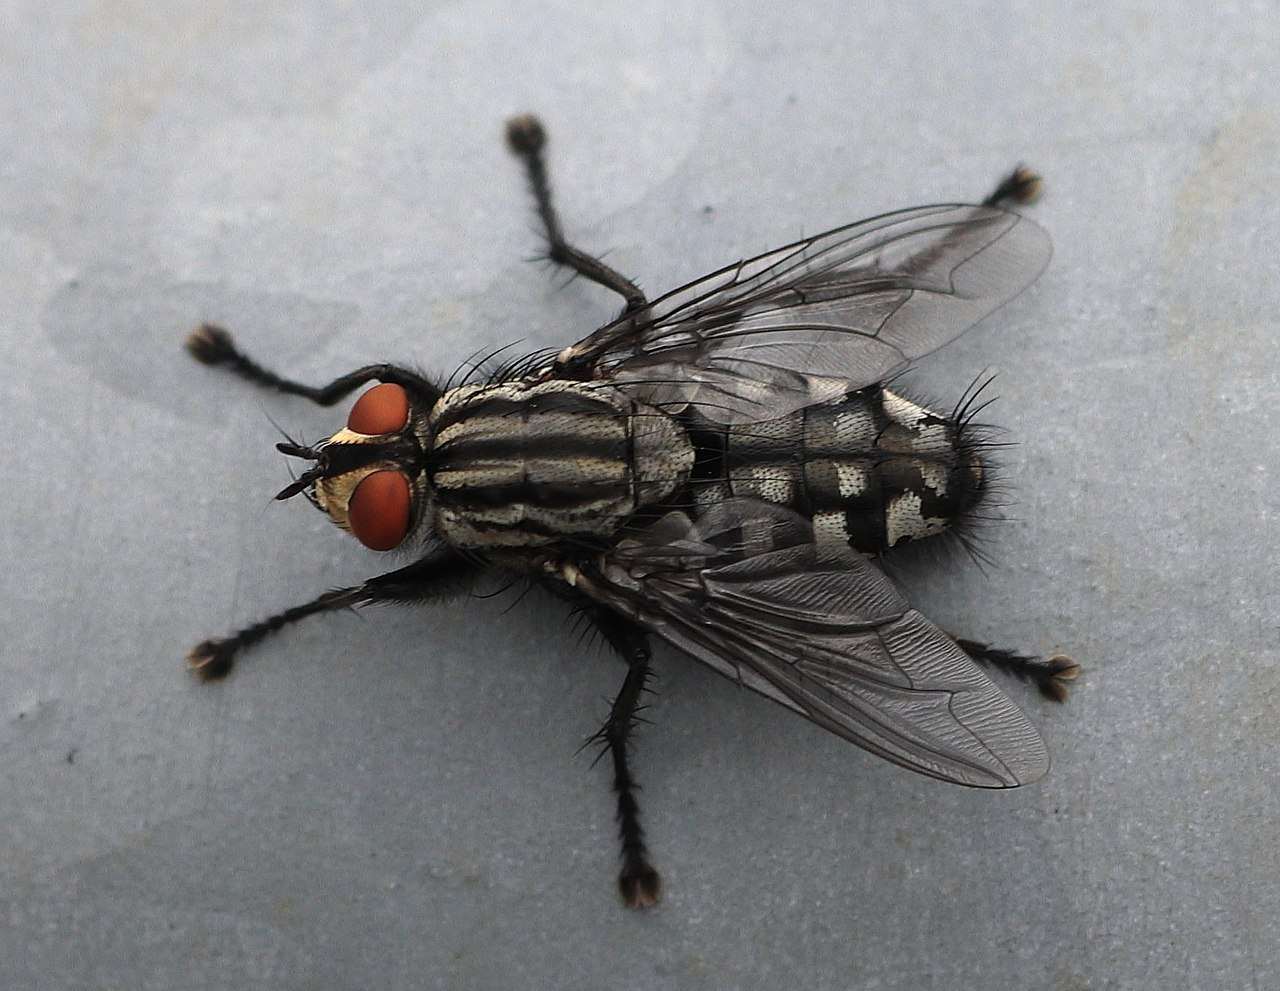
\includegraphics[height=4cm]{flesh-fly.jpg}
        \caption{A Flesh-fly}
        \label{fig:flesh-fly}
    \end{minipage}%
    \begin{minipage}{.5\textwidth}
        \centering
        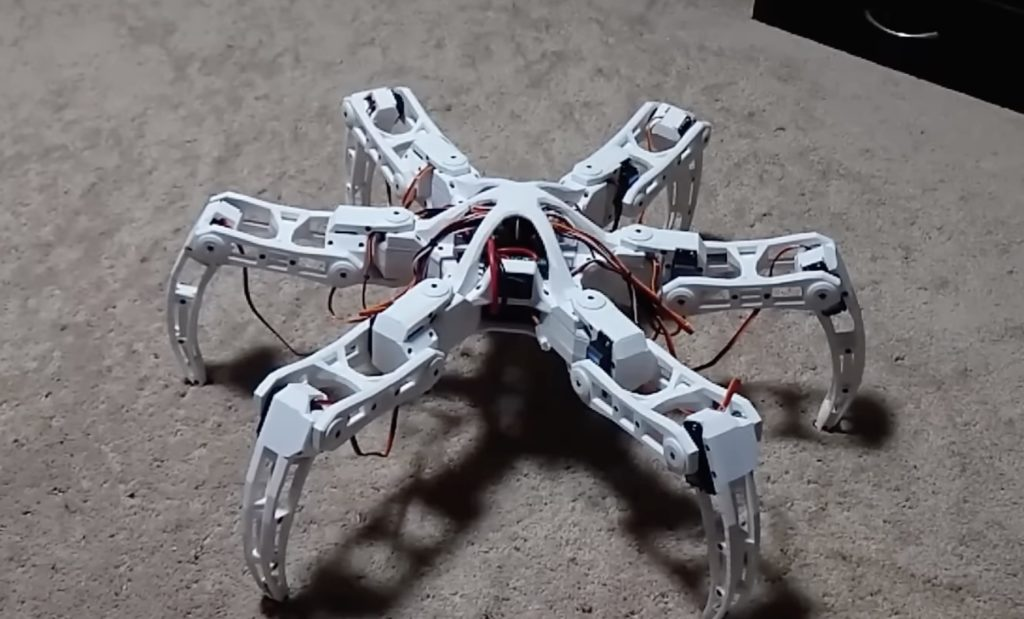
\includegraphics[height=4cm]{circ-hexapod.jpg}
        \caption{A circular hexapod}
        \label{fig:circ-hexapod}  
    \end{minipage}
\end{figure}

In the context of robotics "Hexapod" is used to refer to any robot with six legs, the most common configuration of Hexapods are either a rectangular
layout with three legs on either side mimicking biological Hexapoda, or a circular design with radially symmetrical leg spacing,
as seen in \autoref{fig:circ-hexapod}

The hexapod possess the minimum number of legs to allow a naturally stable platform since while taking a step there can be upwards of three anchor points around the center of mass at all times.
This makes the hexapod hexapods an ideal platform to navigate complex terrain while maintain stability, without requiring advanced balancing control systems.

For a hexapod to walk it must lift some of its legs while bracing with others, the number of swinging to bracing legs, and how each is moved, is referred to as the walking "gait".
The chosen gait influences the speed and stability of the hexapod, the tripod gait is considered to be the most well rounded, having good speed and stability.
In the tripod gait three legs are bracing while the remaining three swing. A example of a more stable gait would be the One by One gait, where only one leg is moved at a time.

It is also possible to create a system where there is no predetermined gait, but rather the system determines the optimal legs to brace and swing depending on the current walking environment.

\section{Control}
Walking over rough terrain requires a control system to correctly actuate the hexapods legs. Various types of control schemes exist, the primary schemes are traditional controllers,
bio-inspired controllers and \ac{rl}. These three schemes are discussed below. Control trends can be seen in \autoref{fig:control-trends}
\begin{figure}[h]
    \centering
    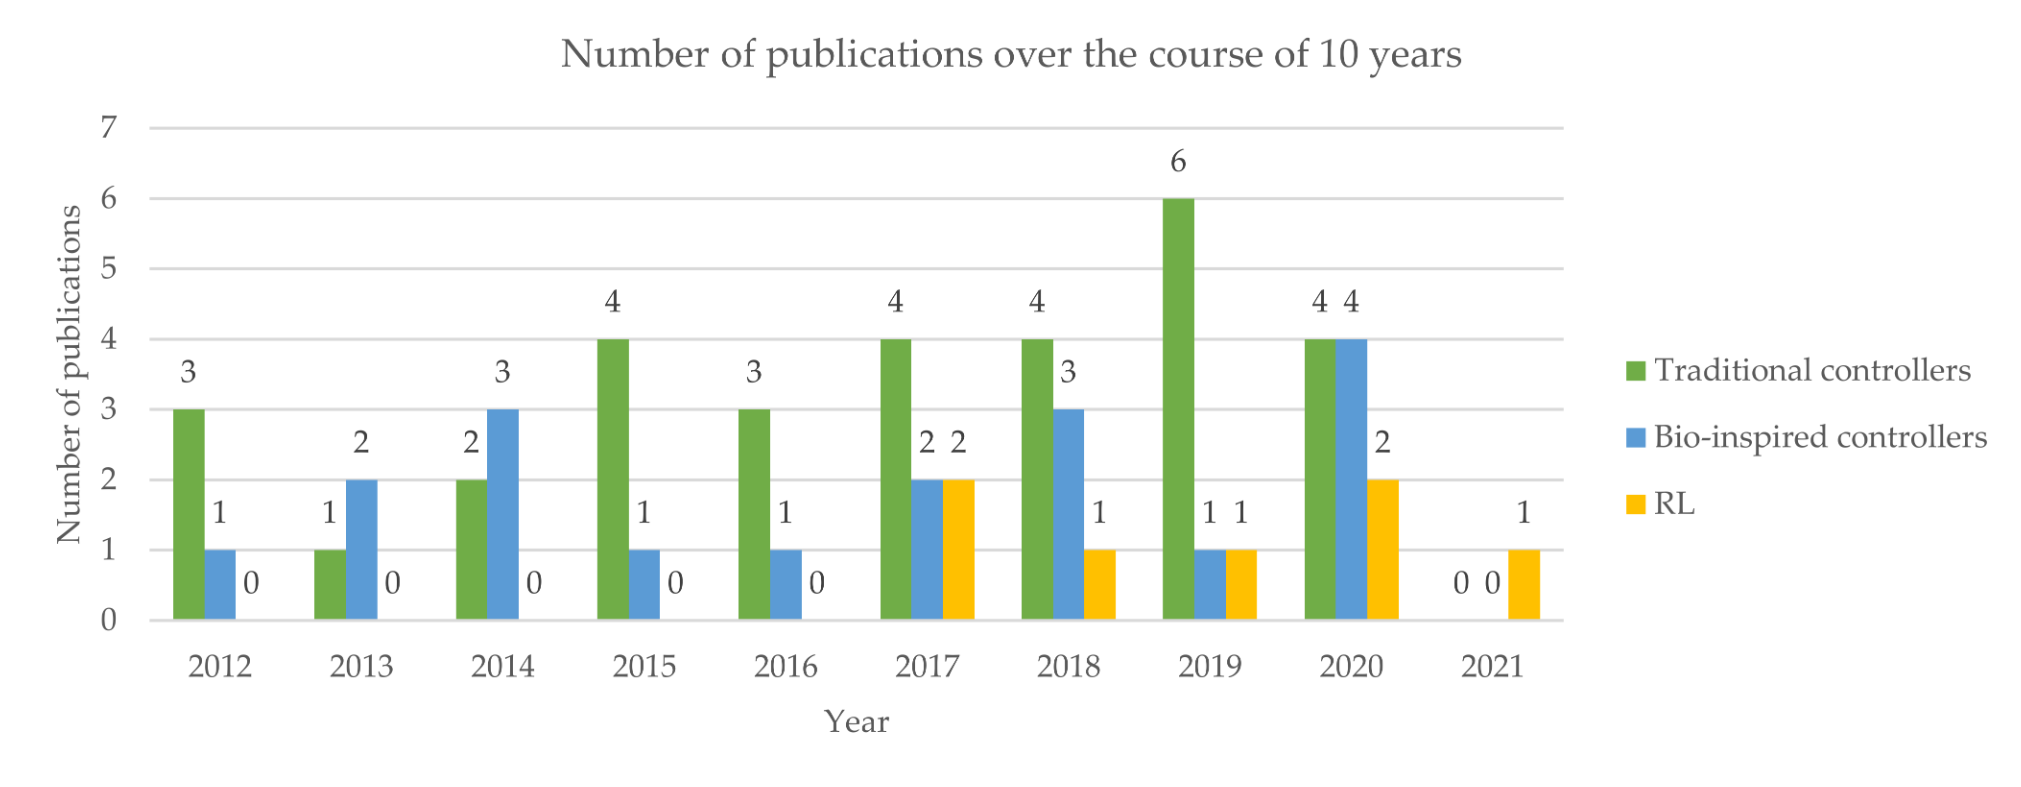
\includegraphics[width=\textwidth]{contoroller-trends.png}
    \caption{Trends of hexapod control schemes \citep{coelho2021trends}}
    \label{fig:control-trends}
\end{figure}

    \subsection{Traditional}
    Traditional controllers rely on an exact mathematical model of the robot and \ac{ik} to calculate angular commands for all leg joints. This method of control is purely kinematic does not 
    take into account external forces applied to the robot, thus it does not inherently adjust to the environment.

    Instead of a purley kinematic model, a dynamic model can also be used. Using a dynamic model the forces acting on the robots legs are taken into account, usually acquired through torque measurements 
    from servos. By taking applied torque into account dynamic model controllers will intrinsically detect a deviation when an external force is applied to the robot or its legs and compensate appropriately.

    It should be noted that it is possible for a kinematic model controller to also adjust to external disturbances, but this is not intrinsic to the control model and requires additional control logic.
    
    \subsection{Bio Inspired}
    Bio inspired controllers attempt to mimic the neural structure of animals to achieve the same locomotion methods that they use. This is implemented through the use of a \ac{ann}
    If implemented successfully a bio inspired controller can be highly adaptable to the surrounding environment and is even able to adapt to damaged or missing legs.

    \subsection{\acl{rl}}
    \ac{rl} controllers are created through using trial and error to construct a neural net that minimises a cost function for a specific goal. This theoretically allows \ac{rl} controllers to adapt to any
    circumstances given enough time, allowing a very hight level of autonomy, as no prior direction is required. \ac{rl} controllers are though notoriously difficult to train properly, especially when the 
    amount of sensors and control outputs grow large, increasing the feature space. And event he most well trained \ac{rl} agent still has the possibility to exhibit inexplicable behaviour.
    
\section{Sensors}
    No matter the control scheme used, to know where to place its feet the robot requires sensor(s) to sense its environment in some way, this could be achieved through simple sensors such as servo torque or touch,
    as used in \cite{t}. Or more advanced methods such as vision or \ac{lidar} could be used, as shown in \cite{t}.

    Depending on the terrain navigation system it might be required to localise the robot in 3D space, for this it is possible to use external sensors such as a type of beacon (RF, Reflective, Ultrasonic), \ac{gps}
    or, through the use of a \ac{slam} system, internal sensors, such as vision could be used.

    The 

    \subsection{End Effector Placement Method}

    Among other research focused on hexapods, many focus on topics such as obstacle avoidance, climbing surfaces, confined surfaces and cargo transportation.
    When focusing of terrain adaptation most often the use of sensors such as \ac{lidar}, torque, or touch are employed. Where usually the height of end effectors
    are adjusted to the height of the terrain \cite{coelho2021trends}.

    Some papers, such as \cite{homberger2017terrain} utilise stereoscopic vision, in addition to end effector height adjustment, also focus on surface material classifications based on which the virtual
    stiffness of the impedance controller is adjusted.

    The focus of this paper will be on end effector height and planar position adaptation through real time walkability classification of the environment. 
    While only utilising an \ac{rgbd} camera as sensor

    \subsection{Localisation and Mapping}

    This project requires a system that will localise the robot within its environment, as the primary sensor used is an \ac{rgbd} camera various visual \ac{slam} systems 
    were considered. ORB-SLAM 3, a optimisation-based, sparse map \ac{slam} system was chosen to be used. ORB-SLAM 3 maintains a sparse map, an atlas, of both active and
    dormant features. This atlas is used to localise in the sparse map \citep{macario2022comprehensive}.

    The implementation of a dense map to be used for end effector placement is discussed in \autoref{chap:mapping}.

\section{Simulation Environment}

The most popular physics simulators for robotics in recent times are Gazebo, \ac{mujoco} and CoppeliaSim (previously V-REP) \citep{Collins-2021}.
Gazebo and CoppeliaSim both have easy to use \ac{gui} interfaces and easy integration with \ac{ros}. \ac{mujoco} on the other hand does not have
a full \ac{gui} interface, only a simulation viewer, and does not have native \ac{ros} integration. Having said this \ac{mujoco} was found to be
the most accurate and fastest simulator when considering the use case of robotics \citep{Erez-2015}.

Considering that the only relevant downside to \ac{mujoco} is the lack of native \ac{ros} integration and the lack of a comprehensive \ac{gui},
which seeing as \ac{mujoco} has good python bindings, could be seen as a advantage, \ac{mujoco} was chosen as the simulator.

% \chapter{Content chapter}

Unless the chapter heading already makes it clear, an introductory paragraph that explains how this chapter contributes to the objectives of the report/project.

\section{Heading level 2}

\subsection{Heading level 3}

\subsubsection{Deepest heading, only if you cannot do without it}
\vspace{2cm}

\paragraph{Equations:}

An equation must read like part of the text. The solution of the quadratic equation $ax^2+bx+c=0$ given by the following expression (note the full stop after the equation to indicate the end of the sentence):
\begin{equation}
    x = \frac{-b \pm \sqrt{b^2-4ac}}{2b} .
\end{equation}
In other cases the equation is in the middle of the sentence. Then the paragraph following the equation should start with a small letter. Euler's identity is 
\begin{equation}
    e^{i \pi} + 1 = 0 ,
\end{equation}
where $e$ is Euler's number, the base of natural logarithms.

The \texttt{amsmath} has a wealth of structure and information on formatting of mathematical equations.

\pagebreak
\paragraph{Symbols and numbers:}

Symbols that represent values of properties should be printed in italics, but SI units and names of functions (e.g. sin, cos and tan) must not be printed in italics. There must be a small hard space between a number and its unit, e.g. \qty{120}{km}. Use the \texttt{siunitx} package to typeset numbers, angles and quantities with units:
\begin{tabbing}
\hspace*{\parindent}\=\verb|\qty{20}{N.m}|\quad\=$\rightarrow$\quad\=\kill
    \>\verb|\num{1.23e3}| \>$\rightarrow$\> $\num{1.23e3}$ \\
    \>\verb|\ang{30}|     \>$\rightarrow$\> $\ang{30}$ \\
    \>\verb|\qty{20}{N.m}|\>$\rightarrow$\> $\qty{20}{N.m}$
\end{tabbing}

\paragraph{Figures and tables:}
The \texttt{graphicx} package can import \texttt{PDF}, \texttt{PNG} and \texttt{JPG} graphic files.

\begin{table}[htbp]
    \centering
    \caption{Standard ISO paper sizes}
    \label{tab:paper}
    \begin{tabular}{lcccc}
    \hline
        Paper\quad && \multicolumn{3}{c}{Sizes} \\
    \cline{2-5}
        &&  $W$      && $H$ \\
        && \small [mm] &&  \small [mm]   \\
    \cline{1-1}\cline{3-3}\cline{5-5}
        A0 && 841 && 1189 \\
        A1 && 594 &&  841 \\
        A2 && 420 &&  594 \\
        A3 && 297 &&  420 \\
        A4 && 210 &&  297 \\
        A5 && 148 &&  210 \\
    \hline
    \end{tabular}
\end{table}


\begin{figure}[htbp]
    \centering
    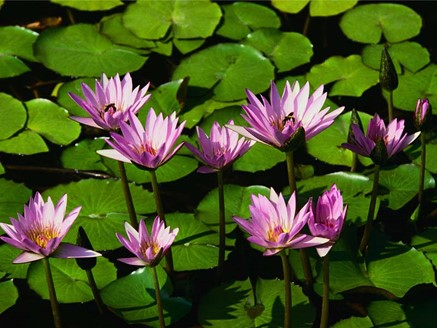
\includegraphics[scale=0.75]{figs/waterplants}
    \caption{Water plants}
    \label{fig:waterplant}
\end{figure}

\chapter{System Overview}
This chapter provides a high level overview of the hexapod, starting with the hardware, then the software, and finally the simulation
environment.
\section{Hardware}
The physical hexapod is primarily the same hexapod described in \cite{erasmus2023guidance}, this robot is shown in figure \ref{fig:hexapod}. For computation, a JetsonNano and Teensy2.0 \ac{mcu} is used. Actuation of the six, three degrees of freedom, legs is handled by 24 Dynamixel RX-64 servos. Sensing is handled by a Realsense D435i \ac{rgbd} camera, which includes a \ac{imu} (However the \ac{imu} is not utilised in this project.) Two Marvelmind ultrasonic \ac{lps} beacons are also present on the robot, although these are not used either.
\begin{figure}[h]
    \centering
    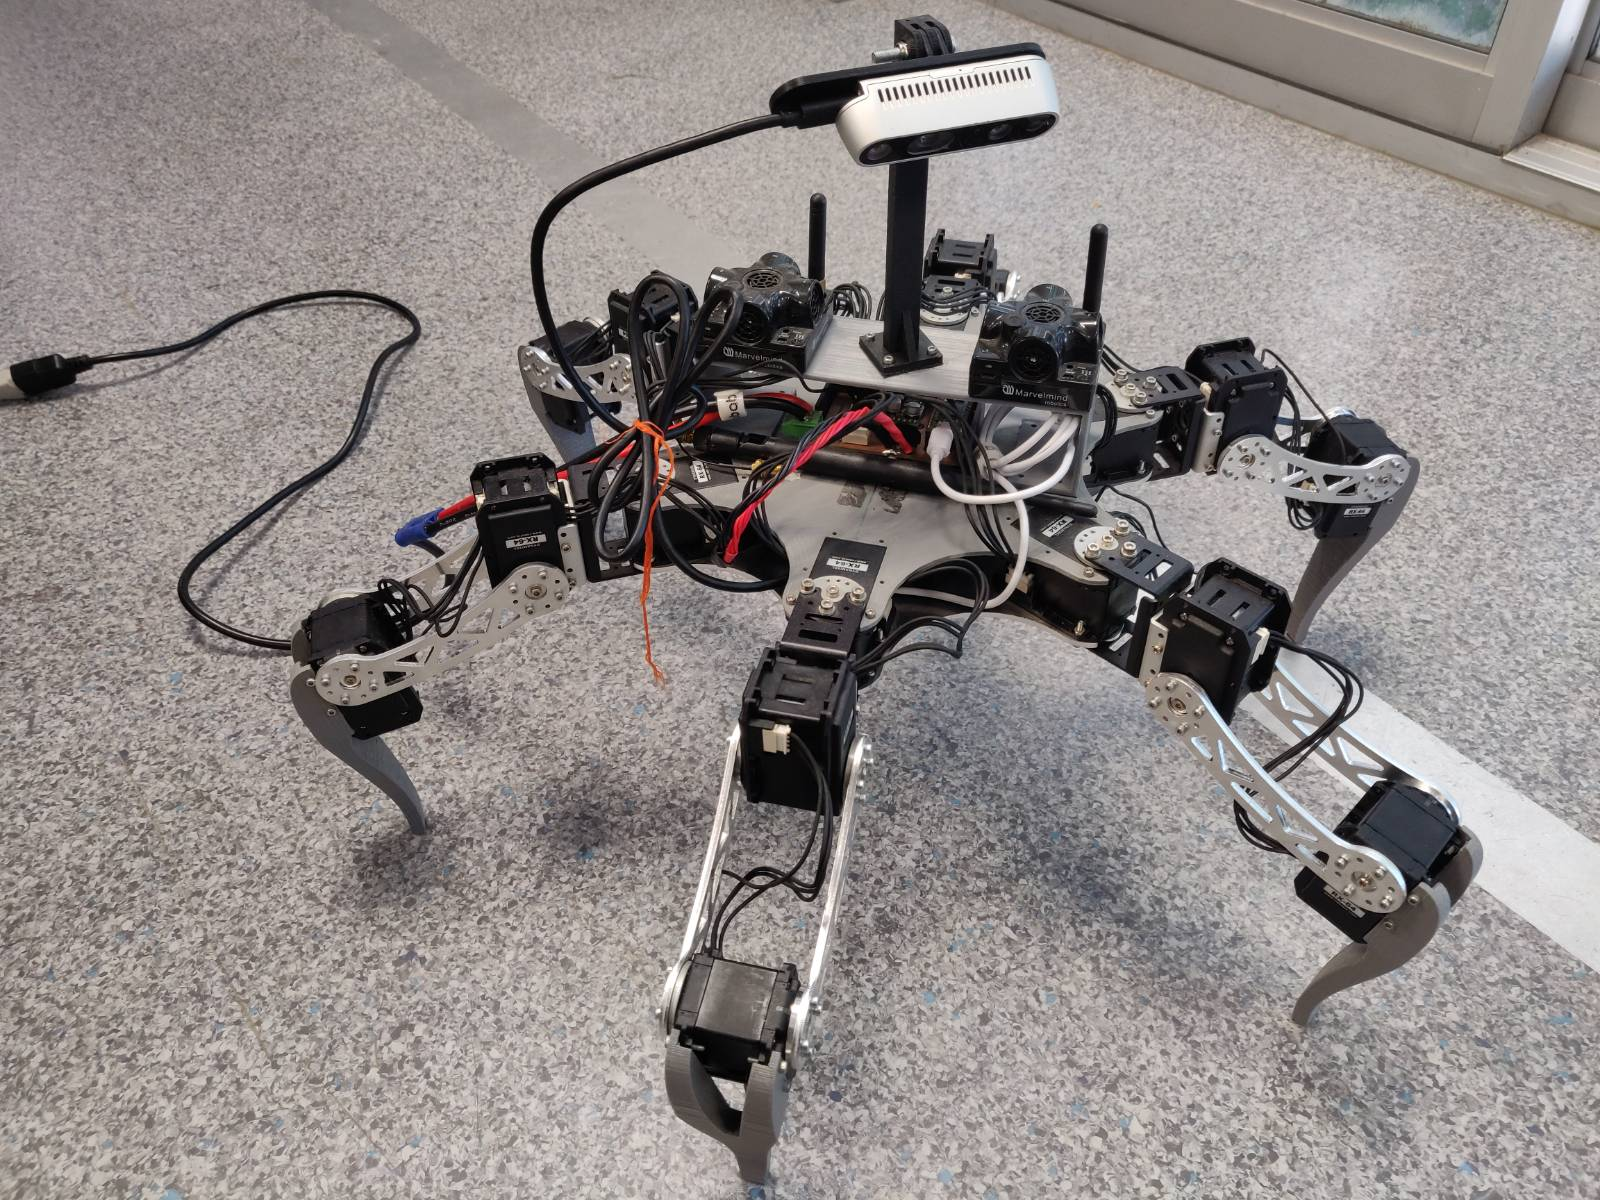
\includegraphics[height=6.6cm]{hexapod.png}
    \caption{Physical Hexapod}
    \label{fig:hexapod}
\end{figure}

\noindent
The only alterations made from the version describe in \cite{erasmus2023guidance} is the thickening of the wires powering the JetsonNano,
to prevent a voltage drop, and the replacement of the 3D printed legs with laser-cut aluminium legs, to prevent leg flexure.

A power cable is shown running to the left and going off image. All tests were conducted using 14.8V
from a bench power supply plugged into the battery port. This was done for convenience and can easily be swapped for a battery.

\section{Software}
The most basic software flow for a robot walking over flat terrain is shown in figure \ref{fig:basic_sys}. This system does not sense
its environment in any way and simply moves its feet along predetermined paths.
\begin{figure}[h]
    \centering
    % \hspace{-1.38cm}
    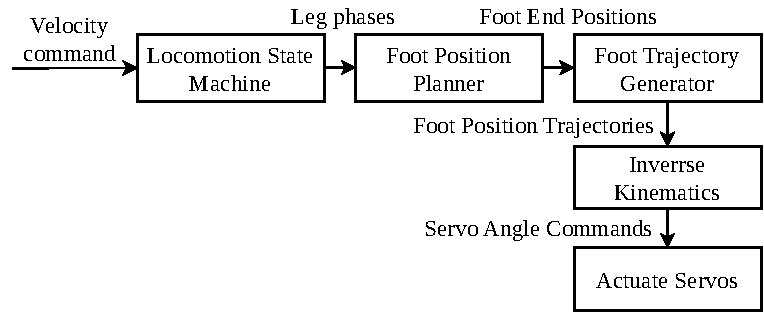
\includegraphics{Diagrams-SysDiffBlockBefore.drawio.pdf}
    \caption{Basic motion system operation.}
    \label{fig:basic_sys}
\end{figure}

\noindent
This basic system will work well enough for walking over flat terrain, but will struggle once any
deviation in terrain height is present. Thus, the proposed, more advanced system, operates with the flow shown in figure \ref{fig:adv_sys}.

The advanced system uses similar components as the basic system, but with the foot end position planner modified to incorporate
checks against a score map and a height map to validate, and if necessary, adjust the foot 
end positions to place the feet at suitable positions in the  terrain. If no suitable adjusted foot positions and trajectories
can be found given the terrain, then the hexapod does not execute the motion and freezes in place. The human operator or
high-level guidance system must then change the overall path of the hexapod. However, this is outside the scope of the current
project.

\newpage
\begin{figure}[h]
    \centering
    % \hspace{-1.38cm}
    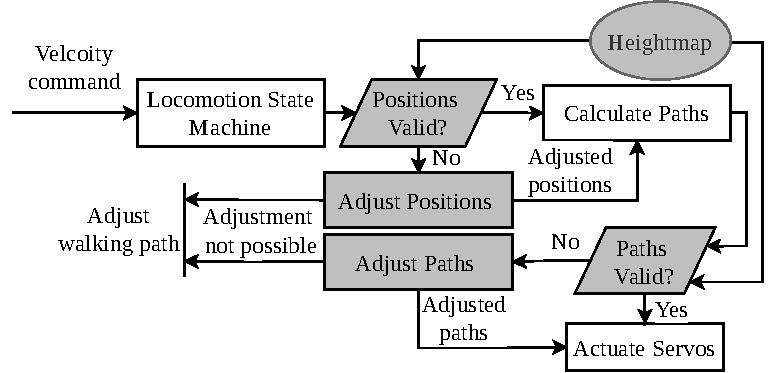
\includegraphics{Diagrams-SysDiffBlockAfter.drawio.pdf}
    \caption{Advanced motion system operation.}
    \label{fig:adv_sys}
\end{figure}

\noindent
The goal of maneuvering uneven terrain is achieved by a combination of 4 primary systems, namely a mapping, 
foot placement optimisation, motion control and a localisation system. A high-level overview of the system implementation can be seen
in figure \ref{fig:system_diagram}.
\begin{figure}[h]
    \centering
    % \hspace{-1.38cm}
    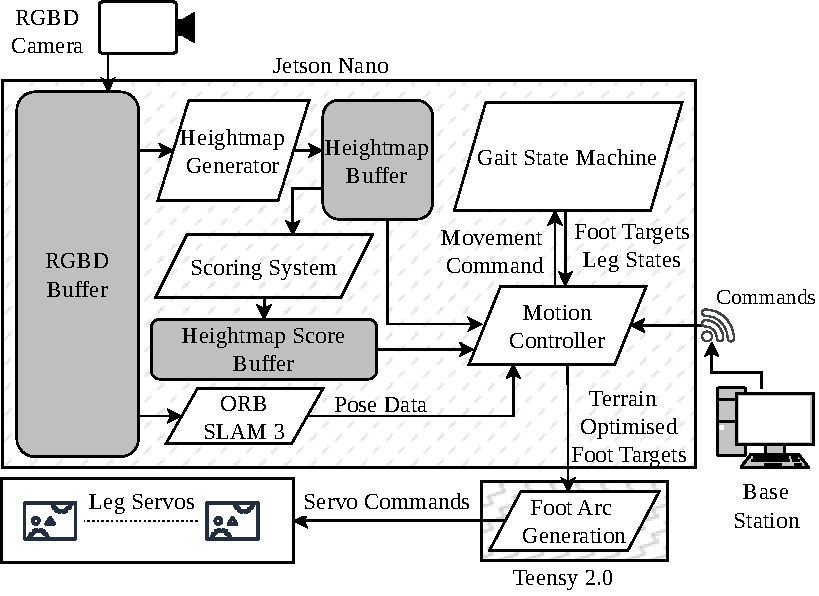
\includegraphics[width=0.93\textwidth]{HexapodSystemDiagram.drawio.pdf}
    \caption{Physical system diagram}
    \label{fig:system_diagram}
\end{figure}

\noindent
The mapping system utilises the \ac*{rgbd} camera to construct a dense heightmap of the immediate surroundings of the robot. As the robot moves around, old data is erased to make way for new data. The size and resolution of the heightmap is adjustable to the available memory and computational power. The heightmap system is further covered in chapter \ref{chap:mapping}.

The foot placement optimisation system takes the heightmap as input and produces another map of equal size to the heightmap. This new map is the score map and is found by assigning a score to each cell of the heightmap. The score is dependant on how stable a position the cell would be for the robot to place its feet. The score map can then be used to evaluate, and adjust if necessary, the initial foot placement proposed by the motion system. The foot placement optimisation system is further covered in chapter \ref{chap:optimisation}.

All the movement of the robot is handled by the motion system, it is comprised of a gait state machine, a foot end position planner, a foot trajectory generator, and inverse kinematics. The gait state machine selects the swinging and supporting legs during for each step to achieve a tripod gait. The foot position planner calculates the nominal foot end positions based on the stepping parameters, namely stride length and step height, but without taking the terrain into account. Simple linear motion is not acceptable for the swinging feet, thus the foot arc generator produces a movement vector based on the remaining distance to a foot's destination, which if followed, results in an arc-like motion to the destination. Finally to execute any movements, positions must be converted to servo angle commands, and the foot velocities must be converted to servo angular rates, using the inverse kinematics equations. The motion system is covered in more detail in chapter \ref{chap:motion}.

% \newpage
\section{Simulation}
As said in section \ref{sec:sim_research}, various simulation environments were considered, but finally \ac{mujoco} was chosen due to its excellent contact physics simulation. The simulation of the hexapod includes the 24 servos, simulated as high gain, high damped angle controlled motors. The \ac{rgbd} camera is also simulated as a direct OpenGL rendering of the simulation environment. As the camera is a OpenGL rendering, all standard buffers used for rendering is generated, this includes the depth buffer. A SLAM system does not run in the simulation, rather simulated estimation noise, based on \cite{macario2022comprehensive}, is added to the true position and orientation directly taken from the simulation.

\newpage
\noindent
The software running on the simulation is largely equivalent to that running on the physical system, with only slight modification to integrate with the simulation instead of the hardware.
Figure \ref{fig:mujoco} shows a screenshot of the simulation environment
\begin{figure}[h]
    \centering
    % \hspace{-1.38cm}
    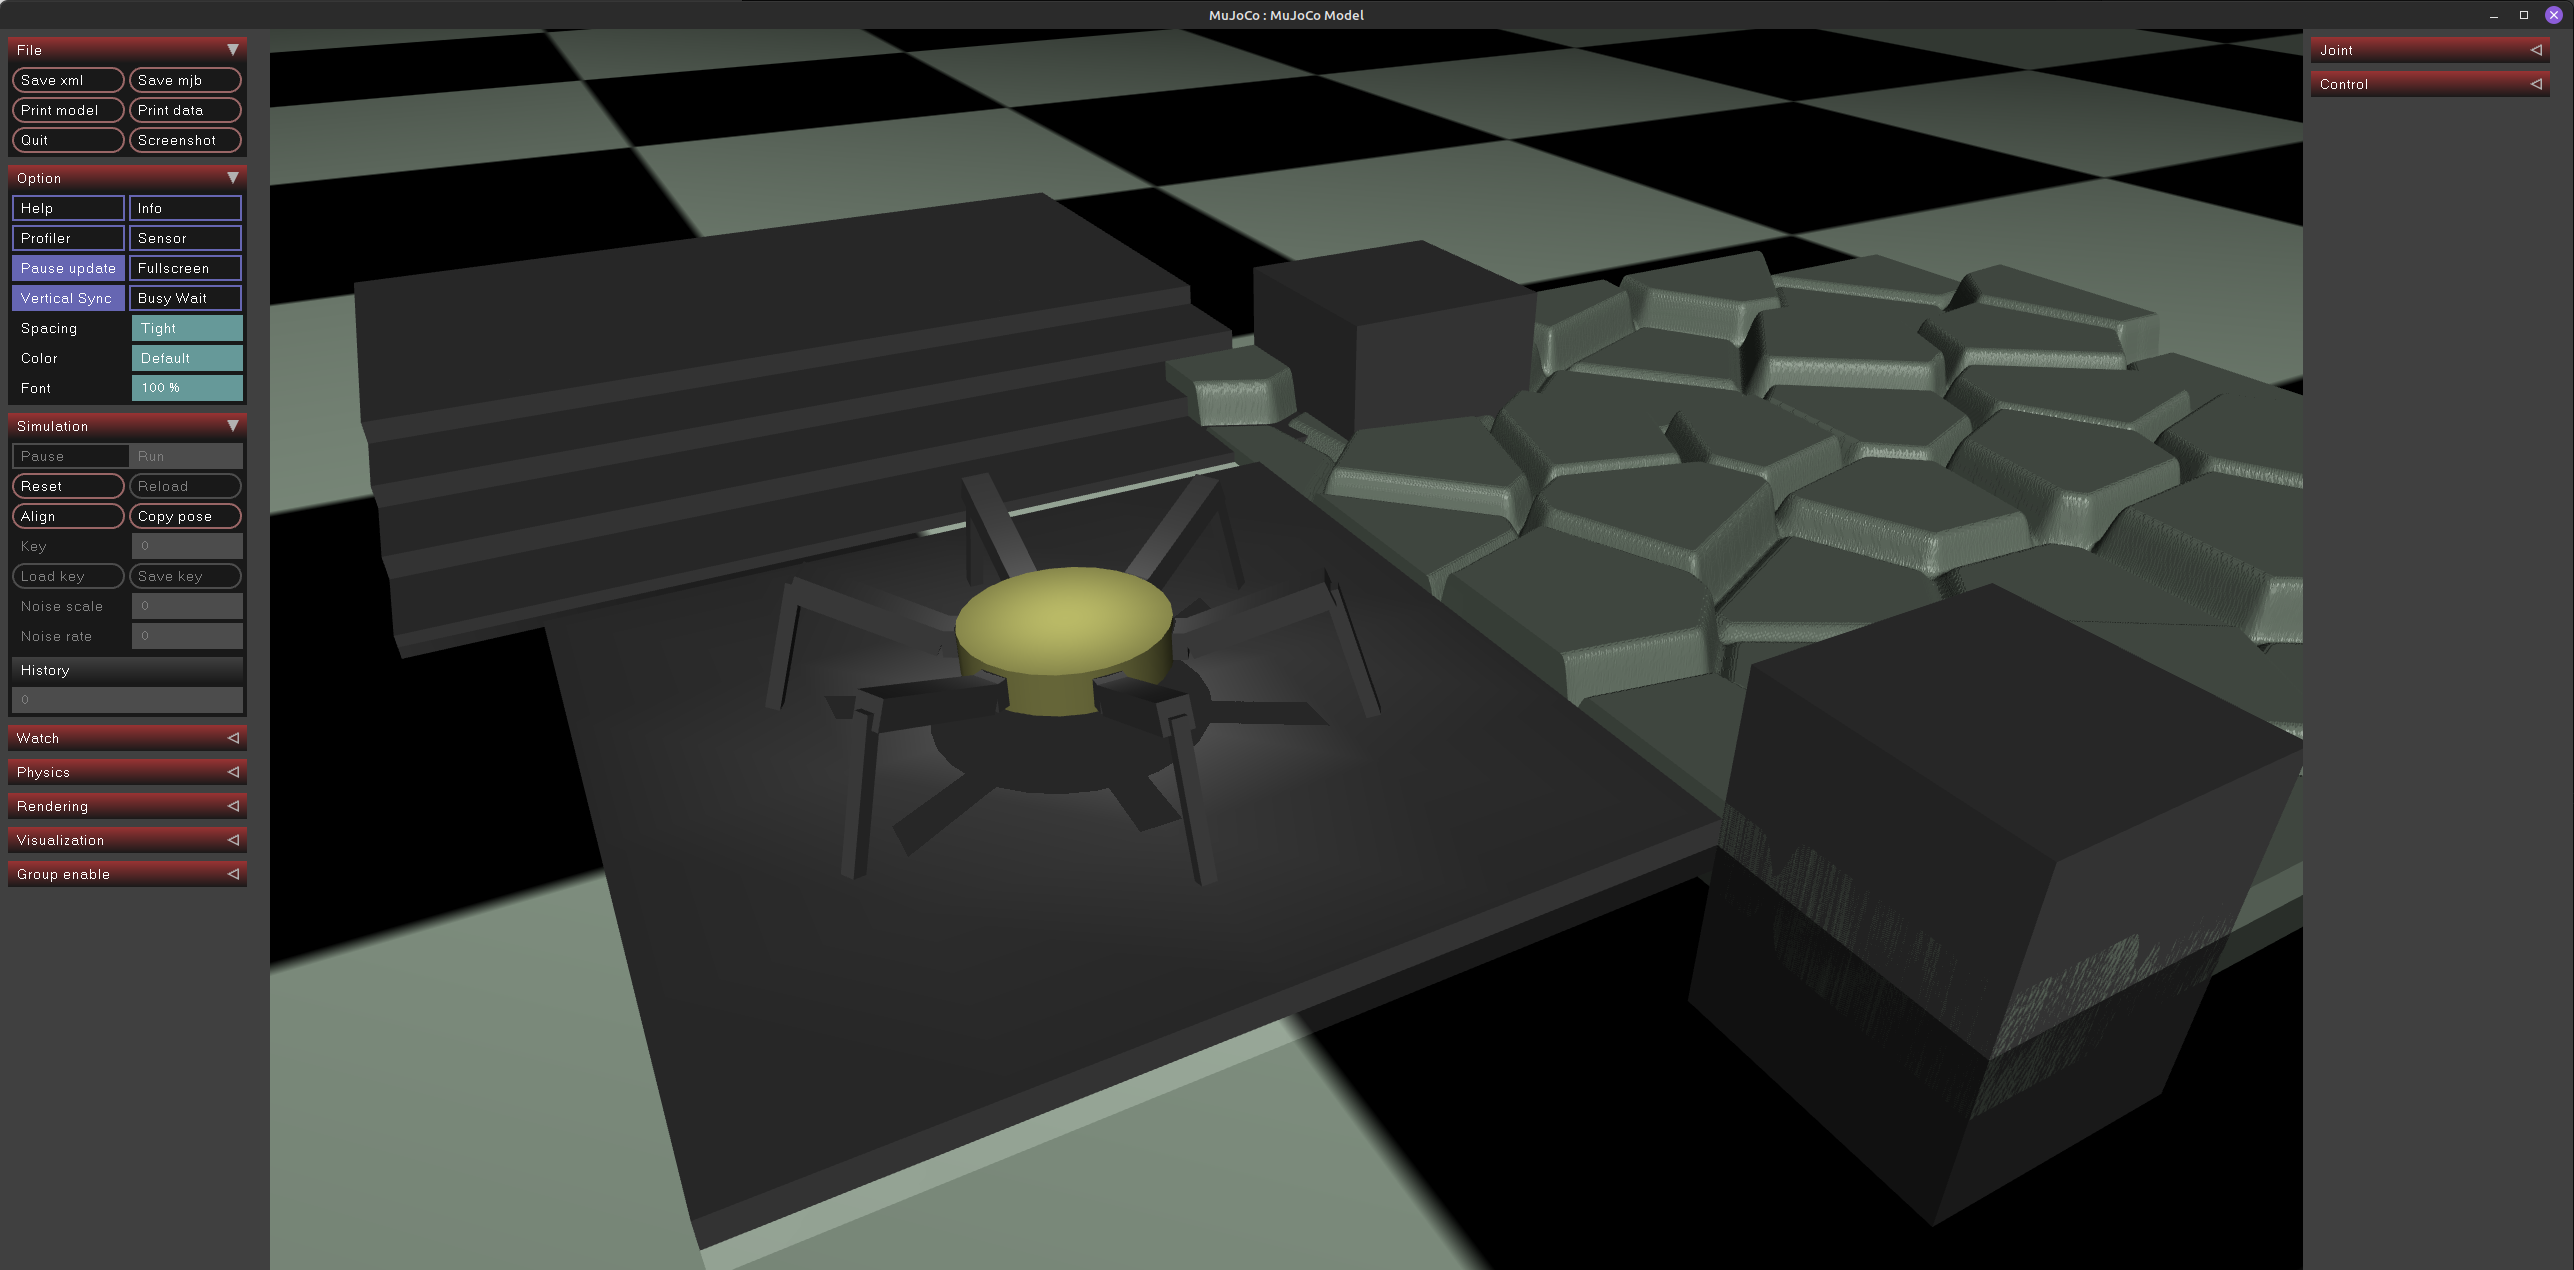
\includegraphics[width=\linewidth]{mujoco.png}
    \caption{The MuJoCo simulation environment}
    \label{fig:mujoco}
\end{figure}

% \bigskip
% \bigskip
% \hrule
% \smallbreak
% \hrule

\chapter{Mapping} \label{chap:mapping}
For accurate foot placement and localisation purposes the robot makes use of two maps, a sparse map covering a large area, and a dense map covering a small
area around the robot. The primarily use of the sparse map is for localisation and extracting pose data, i.e. orientation, velocity and rate. While the dense
map is used to analyse the terrain and find an appropriate point to place the three supporting feet.
It is possible to also use the sparse map for autonomous navigation, however this use case in not covered in this paper.
This chapter covers the design of the mapping system.

The localisation, sparse mapping and pose estimation is handle by ORB-SLAM3 as described in \cite{campos2021orb}. Since ORB-SLAM3 is not a system designed by the author, its
design will not be covered in this chapter. Implementation and operation details will however be covered in chapters \ref{chap:hardware} and \ref{chap:results}.

\section{Projection}
In order to generate a heightmap from a \ac{rgbd} image, it is first required to project the \ac{rgbd} image into 3D space, this is necessary because a heightmap is essentially a 3D environment,
that can be represented as a image due to the assumption of purely convex geometry. 

The camera can be described by its intrinsic and extrinsic parameters. Extrinsic parameters characterise the
cameras position in 3D space, and intrinsic parameters characterise the relationship between the image plane 3D space, 
assuming the camera is at the world origin and an zero rotation. \cite{hartley2003multiple}.

\newpage
\noindent
Refer to figure \ref{fig:projection} as a visual aid regarding projection. Note that this figure is drawn from the perspective of projecting from the image plane into the world,
if the objective was to project from the world onto the image plane the projection center and image plane would swap places, causing the image to be inverted, thus, this figure assumes
that the image rotation has been corrected.
\begin{figure}[h]
    \centering
    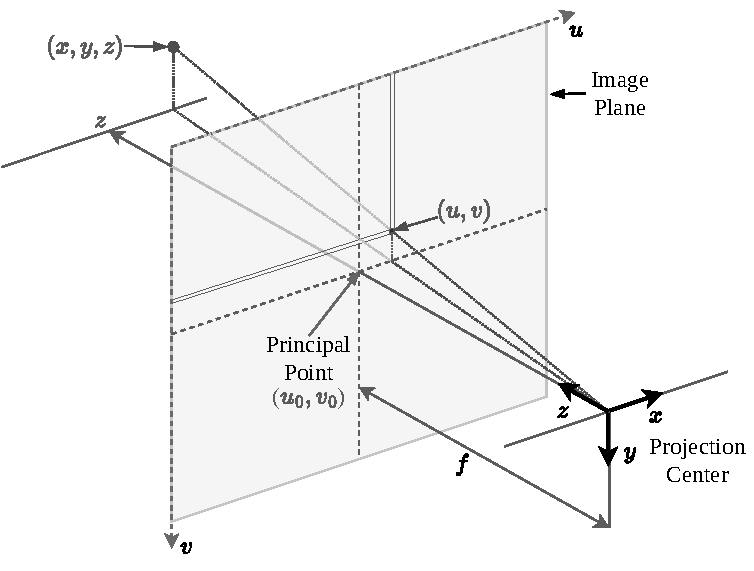
\includegraphics{Diagrams-Projection.drawio.pdf}
    \caption{Camera Projection}
    \label{fig:projection}
\end{figure}

\noindent
Together the extrinsic and intrinsic matrices form the projection matrix,
as shown in equation \ref{eq:projection_matrix},
\begin{equation} \label{eq:projection_matrix}
    \boldsymbol{P} = \boldsymbol{K}
    \begin{bmatrix}
        \boldsymbol{R} & \boldsymbol{T}
    \end{bmatrix}
\end{equation}
where \(\boldsymbol{K}\) is the intrinsic matrix and \(\begin{bmatrix} \boldsymbol{R} & \boldsymbol{T} \end{bmatrix}\) the extrinsic matrix, these are described
in equation \ref{eq:intrinsic} and \ref{eq:extrinsic}.

The projection matrix can be used to project a point on the image plane into world space as shown in equation \ref{eq:full_projection}.

\begin{equation} \label{eq:full_projection}
    \begin{bmatrix}
        u \\
        v \\
        1
    \end{bmatrix}
    = \boldsymbol{P}
    \begin{bmatrix}
        x \\
        y \\
        z \\
        1
    \end{bmatrix}
\end{equation}
where \(u,v\) are the pixel coordinates on the image plane and \(x,y,z\) are the coordinates in world space.
\begin{equation} \label{eq:intrinsic}
    \boldsymbol{K} =
    \begin{bmatrix}
        \alpha_x & \gamma   & u_0 \\
        0        & \alpha_y & v_0 \\
        0        & 0        & 1
    \end{bmatrix}
\end{equation}
where the focal length is represented by,
\[\alpha_x = f \cdot m_y\]
\[\alpha_y = f \cdot m_x\]
with \(m_x\) and \(m_y\) being the inverse of the width and height of a image plane pixel, \(f\) the focal length and \(u_0\),\(v_0\) being the principal point, optimally the center of the image plane.
The skew coefficient, \(\gamma\), is often, and in this case, 0.

The extrinsic matrix is as shown below,
\begin{equation}\label{eq:extrinsic}
    \begin{bmatrix}
        \boldsymbol{R} & \boldsymbol{T}
    \end{bmatrix}
    =
    \begin{bmatrix}
        \boldsymbol{R}_{3\times3} & \boldsymbol{T}_{3\times1} \\
        \boldsymbol{0}_{1\times3} & 1
    \end{bmatrix}
\end{equation}
where \(\boldsymbol{R}\) characterises the camera's heading in world space and \(\boldsymbol{T}\) the world origin expressed in 
the camera coordinate frame.

For ease of preprocessing points are first projected into the camera coordinate frame, in other words, the extrinsic matrix is omitted from equation \ref{eq:full_projection}.
The resultant matrix equation is shown in equation \ref{eq:local_projection}.

\begin{equation} \label{eq:local_projection}
    \begin{bmatrix}
        u \\
        v \\
        1 \\
        1/z
    \end{bmatrix}
    = \frac{1}{z}
    \begin{bmatrix}
        f_x & 0 & c_x & 0 \\
        0 & f_y & c_y & 0 \\
        0 & 0 & 1 & 0 \\
        0 & 0 & 0 & 1
    \end{bmatrix}
    \begin{bmatrix}
        x\\
        y\\
        z\\
        1
    \end{bmatrix}
\end{equation}
From equation \ref{eq:local_projection} \(x,y,z\) are found to be show in equation \ref{eq:proj_z} to \ref{eq:proj_y}.
\begin{align}
    z &= I_{u,v} \label{eq:proj_z}\\[0.2cm]
    x &= \frac{z(u - u_0)}{\alpha_x}\label{eq:proj_x} \\
    y &= \frac{z(v - v_0)}{\alpha_y}\label{eq:proj_y}
\end{align}
where \(I_{u,v}\) is the depth image value at pixel coordinates \(u,v\). For later use the variable \(\boldsymbol{p} \inrefframe{C}\) is defined as in equation \ref{eq:pcam},
\begin{equation}\label{eq:pcam}
    \bm{p}\inrefframe{C}=
    \begin{bmatrix}
        x &y &z
    \end{bmatrix}^T
\end{equation}

\newpage
\section{Map Buffer}
    Once the depth image is projected into map space, their x and y coordinates are used as indices to write their z value into the heightmap. The heightmap is stored in
    a 2D circular buffer, this means that as the robot moves around, old map data is erased to make room for new data. This structure is illustrated in figure \ref{fig:memory}.
    \begin{figure}[h]
        \centering
        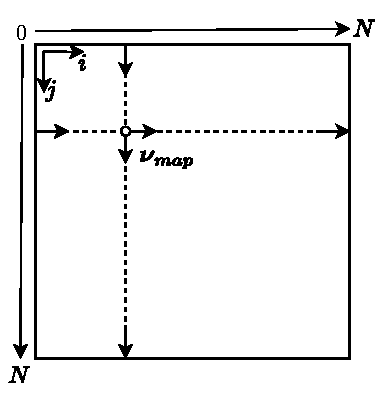
\includegraphics{Diagrams-Memory.drawio.pdf}
        \caption{Memory Diagram}
        \label{fig:memory}
    \end{figure}

    The heightmap buffer, \(\boldsymbol{M}\), is of size \(N \times N\) and is indexed by \(i,j\). In order to write the height value into the heightmap, the camera point in camera space,
    \(\bm{p}\inrefframe{C}\), is translated into map space, \(\bm{p}\inrefframe{M}\), as shown in equation \ref{eq:project_to_map},
    \begin{equation} \label{eq:project_to_map}
        \boldsymbol{p}\inrefframe{M} = \boldsymbol{p}\inrefframe{C} \transframe{C}{M}
    \end{equation}
    see appendix \ref{app:transforms} for transformation definitions.



\chapter{Motion} \label{chap:motion}
% This chapter describes the systems governing the motion of the robot, such as leg motion planning and gait generation.
The basic operation of the motion system is as follows, first the robot is commanded to walk in a certain direction, at a
certain speed and body height. These commands are sent from the base station to Jetson Nano on the robot,
the motion controller node on the Jetson Nano then sends these commands to the gait state machine node, at a fixed frequency.
The gait state machine uses the received direction stride length to generate leg states (swinging or supporting) and the ideal
final position of each foot. These states and positions are sent back to the motion controller node where the positions are adjusted
based on the heightmap data to ensure stable footing. The leg states and adjusted feet positions are then sent to the servo 
controller node, this node controls the servos to move the robots feet to their final positions, either in a arc or linearly,
depending on their state (swinging or supporting). %A high level diagram of the motion system can be seen in \ref{fig:motion_system}.

\begin{figure}[h]
    \centering
    % \hspace{-1.38cm}
    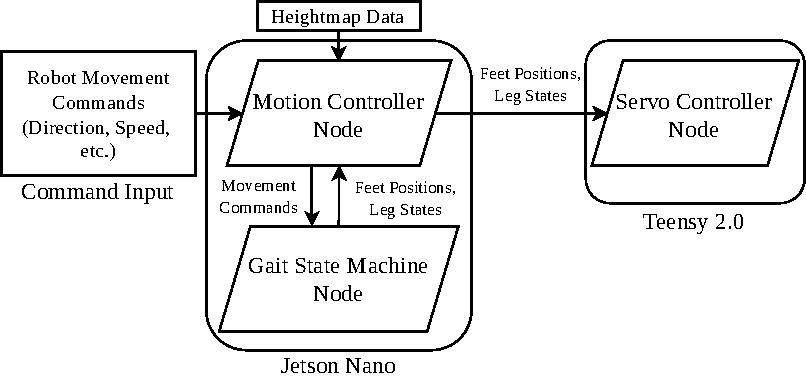
\includegraphics{Diagrams-MotionSystem.drawio.pdf}
    \caption{Motion System Overview}
    \label{fig:motion_system}
\end{figure}

\section{Gait State Machine}
The state machine used to realise the tripod gait used in the robot is quite simple, comprised of only two states, stepping and
resting, as can be seen from figure \ref{fig:gaitSM}. Table \ref{tab:state_defs} defines the actions that should be taken during
each state.

The primary computation done by this state machine is calculating which legs are supporting and which are swinging, which occurs
on entering the "Stepping" state. This function is described in section \ref{sec:supp_swing_calc}.

\begin{figure}[h]
    \centering
    % \hspace{-1.38cm}
    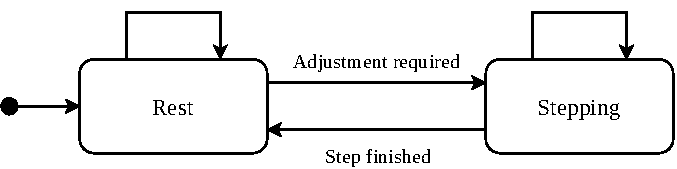
\includegraphics{Diagrams-GaitSM.drawio.pdf}
    \caption{Gait State Machine}
    \label{fig:gaitSM}
\end{figure}

\begin{table}[h]
    \center
    \begin{tabularx}{\textwidth}{|l|X|}
        \hline
        \multicolumn{2}{|c|}{Rest State Definition} \\
        \hline
        Enter Condition & Has all feet reached their targets? \\
        \hline
        On Entering & Set all leg states as supporting. \\
        \hline
        While Active & Do nothing \\
        \hline
    \end{tabularx}
    
    \bigskip
    \noindent
    \begin{tabularx}{\textwidth}{|l|X|}
        \hline
        \multicolumn{2}{|c|}{Stepping State Definition} \\
        \hline
        Enter Condition & Is there a mismatch between feet targets and current position? \\
        \hline
        On Entering & Calculate and set the leg states based on walking direction, see section \ref{sec:supp_swing_calc}. Choose and optimise nominal targets
        for the current step, see chapter \ref{chap:optimisation}\\
        \hline
        While Active & Adjust feet targets based on direction, stride length and robot height, see chapter \ref{chap:optimisation}\\
        \hline
    \end{tabularx}
    \caption{State Definitions}
    \label{tab:state_defs}
\end{table}

\newpage
\subsection{Choosing The Supporting And Swinging Legs} \label{sec:supp_swing_calc}
    The robot body is divided up into sextants, centered around the nominal leg positions. When calculating
    the swinging legs it is first determined in which sextant the movement direction vector falls, this is called the active sextant.
    The leg related with the active sextant, and the two opposite, are then chosen as swinging, with the remaining three legs chosen as supporting.
    The states of the legs are encapsulated by the boolean array, \(\bm{S_i}\), defined by equation \ref{eq:is_swing},
    where a 1 indicates swinging and 0 supporting.
    \begin{equation}\label{eq:is_swing}
        \bm{S}_{\bm{i} - \xi}=[i \text{ is even}]
    \end{equation}
    where \(\xi \in i\) is the active sextant/leg number, and,
    \[i = [\![0..5]\!]\]

    Figure \ref{fig:sextants} illustrates and example with sextant 1 being active. Thus legs 1, 3 and 5 are swinging, while legs 0, 2 and 4 are supporting.
    \begin{figure}[h]
        \centering
        \hspace{1.1cm}
        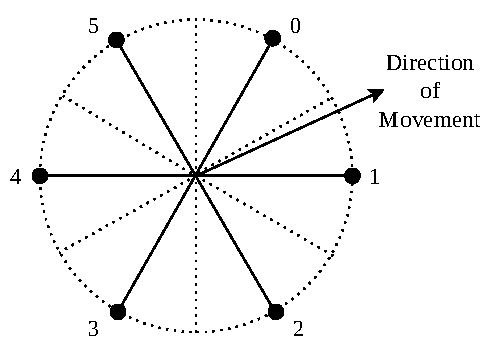
\includegraphics[clip, trim=0 0.25cm 0 0.25cm]{Diagrams-Sextants.drawio.pdf}
        \caption{Leg sextants, with sextant 1 being active.} 
        \label{fig:sextants}
    \end{figure}
    
    \noindent
    This of course would not be sufficient to define a walking gait, as at the end of each step \(\bm{S_i}\) does not invert.
    Thus and additional step after equation \ref{eq:is_swing} is added. The current horizontal length of leg \(\xi\), defined as \(l_\xi\), is compared to its nominal
    horizontal length, \(L_\xi\). If \(l_\xi\ > L_\xi\), invert \(\bm{S_i}\). As shown in equation \ref{eq:negate_is_swing}.
    \begin{equation} \label{eq:negate_is_swing}
        \bm{S}_{\bm{i} - \xi} =
                                            \begin{cases}
                                                \bm{i} \setminus \bm{S}_{\bm{i} - \xi} & l_\xi > L_\xi \\
                                                \bm{S}_{\bm{i} - \xi} & l_\xi \leq L_\xi
                                            \end{cases}\\[0.1cm]
    \end{equation}

    \newpage
    \subsection{Choosing nominal foot positions}    
    Once the active and inactive legs have been selected it is required to choose nominal targets for all the feet. Sections \ref{sec:support} and \ref{sec:swing}
    describe the process for finding the support and swinging leg targets; It should be noted that target matrices, denoted by \(\bm{t}\), are common between these two sections, but are computed
    differently depending on whether the leg is swinging or supporting.
        
    \subsubsection{For Supporting Legs} \label{sec:support}
    For the supporting legs, first the required move vectors, \(\bm{m} \inrefframe{L}\), are calculated in equation \ref{eq:move_vec},
    \begin{equation} 
        \mdim{\bf{m}\inrefframe{L}}{3}{6} = (\bm{T}\inrefframe{L} - l_\text{str} \bm{\bm{w}_\text{dir}}\inrefframe{L}) - \bm{t_\text{nom}}\inrefframe{L} \label{eq:move_vec}
    \end{equation}
    where \(\bm{T}\inrefframe{L}\) contains the constant rest positions the feet, \(l_\text{str}\) is the desired stride length, \(\bm{w}_\text{dir}\inrefframe{L}\)
    contains the desired walk directions, and \(\bm{t}_\text{nom} \inrefframe{L}\) contains the nominal targets.

    Then the optimised targets, \(\bm{t_\text{opt}} \inrefframe{L}\), are calculated as the addition of the previous targets and the move vector in equation \ref{eq:move_vec},
    \begin{equation} \label{eq:opt_supp}
        \mdim{\bf{t}_\text{opt}\inrefframe{L}}{3}{6} = \bm{t}_\text{prv}\inrefframe{L} + \bm{m}\inrefframe{L}
    \end{equation}
    where \(\bm{t}_\text{prv}\inrefframe{L}\) contains the previous, optimised, targets. Note that equation \ref{eq:opt_supp} does not include the optimisation
    function \textcolor{red}{XXXX}, this is because the supporting feet will not move relative to the terrain, and thus do not need optimising.

    \subsubsection{For Swinging Legs} \label{sec:swing}
    For the supporting legs, the nominal targets in map space, \(\bm{t_\text{nom}} \inrefframe{M}\) are calculated as in equation \ref{eq:t_map},
    \begin{equation} \label{eq:t_map}
        \mdim{\bf{t}_\text{nom}\inrefframe{M}}{3}{6} = \bm{T}\inrefframe{L} - \Delta\bm{p}_\text{rob}\inrefframe{L} + \left(l_\text{str}+\avg \bm{m}\inrefframe{L}\right)\bm{w}_{dir}\inrefframe{L} \transframe{L}{M}
    \end{equation}
    where \(\Delta\bm{p}_\text{rob}\inrefframe{L}\) is calculated as the difference between the robot's current position and its position at 
    the beginning of the previous step, as shown in equation \ref{eq:delta_pos}.
    \begin{equation}\label{eq:delta_pos}
        \mdim{\Delta\bm{p}_\text{rob}\inrefframe{L}}{3}{1} = \bm{p}_\text{rob}\inrefframe{W}-\bm{p}_\text{rob prev}\inrefframe{W} \transframe{W}{L}
    \end{equation}
    where \(\bm{p}_\text{rob} \inrefframe{W}\) is the robot's current position, and \(\bm{p}_\text{rob prev}\inrefframe{W}\) is the robot's position at the beginning of the previous step.

    Additionally, for use in equation \ref{eq:move_vec}, the swinging legs nominal targets, \(\bm{t_\text{nom}} \inrefframe{L}\), are calculated as 
    in equation \ref{eq:swing_nom},
    \begin{equation} \label{eq:swing_nom}
        \mdim{\bm{t}_\text{nom}\inrefframe{L}}{3}{6} = \bm{T}\inrefframe{L} - \Delta\bm{p}_\text{rob}\inrefframe{L} + l_{str}\bm{w}_\text{dir}\inrefframe{L}
    \end{equation}

    Note that \(\bm{t}_\text{nom}\inrefframe{M}\) is quite similar to \(\bm{t}_\text{nom}\inrefframe{L}\), the difference is that, 
    assuming the \transframe{M}{L} transform is applied, \(\bm{t}_\text{nom}\inrefframe{M}\) is set such that it
    will align with \(\bm{t}_\text{nom}\inrefframe{L}\)
    at the end of the step. Thus, the omission of the average supporting move vector, \(\avg \bm{m}\inrefframe{L}\), in calculating \(\bm{t}_\text{nom}\inrefframe{L}\)
    in equation \ref{eq:swing_nom}.
    Meaning at until the end of the step \(\bm{t}_\text{nom}\inrefframe{M}\) and \(\bm{t}_\text{nom}\inrefframe{L}\) will point 
    to different positions if world space. This is due to needing to account for body movement in world space, but not in local space.


    \section{Foot Motion} \label{sec:arc_generation}
    When taking a step the foot can not simply be moved to its destination in a straight line, as doing so will cause the foot to be dragged on the terrain,
    impeding the movement of the robot. Thus it is required to move the foot in an arc like motion to clear any obstacles that might be in its path.


    \subsection{Existing System}
        The existing system will, at the start of each step, compute an arc for each foot to follow, this arc is then sent to the servo controller
        to be executed. While efficient and effective in ideal conditions, this method of defining the arc has poor performance when considering external
        influences. If for example the robot has to adjust the final target of its feet mid step, this arc would have to be recomputed in its entirety,
        thus leading to possible performance concerns.

        In addition to this Text, the current system is designed with the assumption that the starting position of the foot is grounded, thus if the arc is recomputed
        mid step the arc will be undesirable, as it will rise with the desired step height for a second time. This is illustrated in Figure \ref{fig:old_arc}.

        \begin{figure}[h]
            \centering
            \hspace{-1.38cm}
            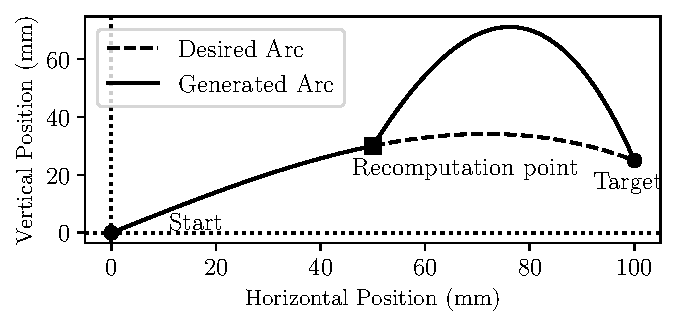
\includegraphics[clip, trim=0 0.25cm 0 0.25cm]{old_path.pdf}
            \caption{Existing arc recomputation problem}
            \label{fig:old_arc}
        \end{figure}

    \subsection{Improved System}
        The improved system solves this problem by utilising a flow function. During a step, this function will continuously calculate the
        direction that the foot must move to reach its destination. Thus this system is resilient to external disturbances and is capable of adjusting to
        varying destination and step height requirements. 
        
        The flow field is designed to first move the foot vertically upwards until horizontal coplanar with the destination, and then to follow a
        arc to the destination with a defined step height, this can be adjusted to make the arc start before or after coplanar. The step height can be adjusted at any point in time and the flow field will adjust accordingly.
        Figure \ref{fig:foot_arc} illustrates the field function and is described in section \ref{sec:flow_function}.
        \begin{figure}[h]
            \centering
            \hspace{-1.38cm}
            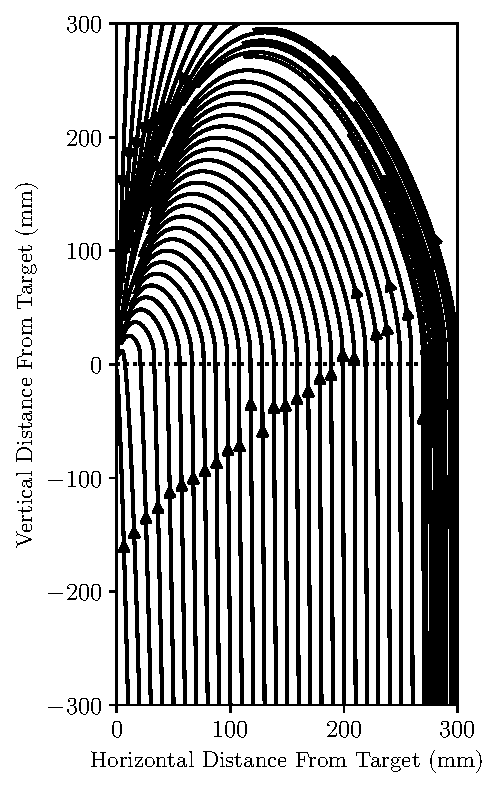
\includegraphics[clip, trim=0 0.25cm 0 0.25cm]{foot_path.pdf}
            \caption{End effector movement path}
            \label{fig:foot_arc}
        \end{figure}

        \subsubsection{Flow Function Description} \label{sec:flow_function}
            The flow function, \(\rho(x,y)\), uses the gradient function of a parabola passing through the point \([0,0]\) and \([x,y]\) as a basis, where point \([x,y]\)
            is the current point that is being evaluated and \(x\) is the horizontal distance between the destination and the current point and \(y\) the
            vertical distance. The final function is described by equations \ref{eq:rho} to \ref{eq:sigmoid}, for the process of designing the flow function
            please see appendix \ref{app:flow_function}.
            \begin{equation} \label{eq:rho}
                \begin{aligned}
                    \rho(x,y) &= \frac{\delta}{\delta x\delta y}&&f_a(x,y)x^2 + f_b(x,y)x + C\\
                    &= &&2f_a'(x,y)x + f_b'(x,y)    
                \end{aligned}
            \end{equation}
            where, %\(f_a'(x,y)\) and \(f_b'(x,y)\) are defined as follows:
            \begin{align} \label{eq:fa}
                f_a'(x,y) &= -\left|\frac{v_h}{x}\right| - \left|S(y)\right|\\
                f_b'(x,y) &= \frac{y}{x} - f_a(x,y)
            \end{align}
            with \(v_h\) being the variable describing the step height and \(S(y)\) being a sigmoid like function 
            responsible for the initial vertical rise. \(S(y)\) is defined in Equation \ref{eq:sigmoid}.
            \begin{equation} \label{eq:sigmoid}
                S(y) = \frac{0.515(y-q)}{1+\left|y-q\right|-0.505}
            \end{equation}
            where \(q\) is the variable that determines at which vertical displacement the leg path transitions from primarily an vertical motion to
            an arc motion. Figure \ref{fig:sigmoid_like} illustrates the sigmoid like function for different values of \(q\).
            \begin{figure}[h]
                \centering
                \hspace{-1.38cm}
                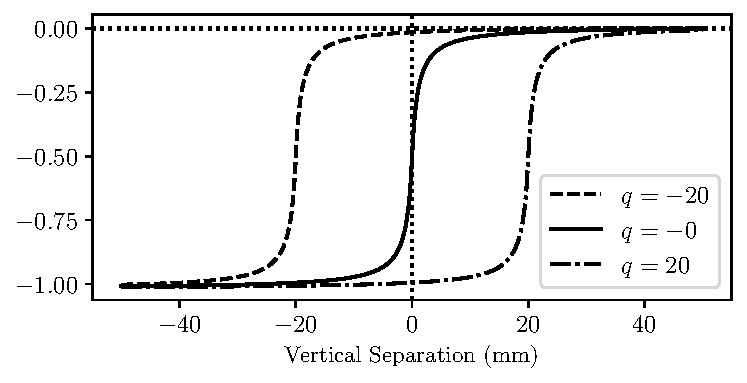
\includegraphics[clip, trim=0 0.25cm 0 0.25cm]{sigmoid_like.pdf}
                \caption{Sigmoid Like}
                \label{fig:sigmoid_like}
            \end{figure}

            \noindent
            Note that the 0.515 and 0.505 values in equation \ref{eq:sigmoid} are set to make its output range from roughly -1 to 0 over the active range.

\newpage
\section{Kinematics}
    When commanding a foot position, the servo controller requires a function to calculate servo angles. While the foot arc planner, see section 
    \ref{sec:arc_generation}, requires the current position of the feet to function. The \ac{ik} and \ac{fk} functions described in this section provide
    this functionality. Figure \ref{fig:kinematics} illustrates the leg geometry and variables used in the \ac{ik} and \ac{fk} functions.
    \begin{figure}[h]
        \centering
        % \hspace{-1.38cm}
        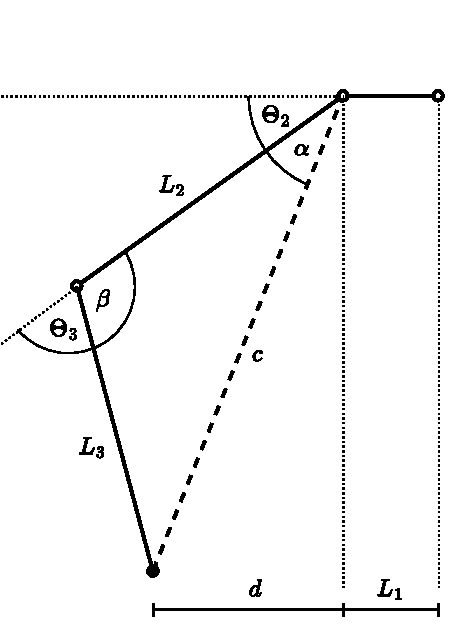
\includegraphics[clip, trim=0 0.25cm 0 1.51cm]{kinematics.drawio.pdf}
        \caption{Leg Kinematics Diagram}
        \label{fig:kinematics}
    \end{figure}

    \subsection{\acf{ik}}
        The \ac{ik} function calculates the leg servo angles, \(\bm{\Theta} = [\Theta_1, \Theta_2, \Theta_3]^T_{\displaystyle ,}\) required
        to move the foot to the given target position vector, \(\bm{t} = [x_t,y_t,z_t]^T_{\displaystyle .}\)
        \hbox{Equation \ref{eq:ik}} describes the \ac{ik} function.
        \begin{equation}\label{eq:ik}
            \bm{\Theta}(x_t,y_t,z_t) =
                                % \begin{bmatrix}
                                %     \Theta_1\\
                                %     \Theta_2\\
                                %     \Theta_3
                                % \end{bmatrix}
                                % =
                                \begin{bmatrix}
                                    \arctan{\left(\dfrac{x_t}{y_t}\right)}\\[0.5cm]
                                    \dfrac{\pi}{4} - \alpha - \arctan{\left(\dfrac{y_t}{d-L_1}\right)}\\[0.5cm]
                                    \dfrac{\pi}{2} - \beta
                                \end{bmatrix}
        \end{equation}
        Where \(\alpha\), \(\beta\), \(c\) and \(d\) are calculate as shown in equations \ref{eq:alpha} to \ref{eq:dik}. For derivations of these variable
        please see \ref{app:kinematic}.
        \begin{align}
            \alpha &= \arcsin{\left(\frac{L_3\sin{\beta}}{c}\right)} \label{eq:alpha} \\[0.5cm]
            \beta &= \arccos{\left(\dfrac{L_1^2 + L_2^2 -c^2}{2L_1L_2}\right)}\\[0.5cm]
            c &= \sqrt{(d-L_1)^2+z_t^2}\\[0.5cm]
            d &= \sqrt{x_t^2 + y_t^2} \label{eq:dik}
        \end{align}
    \subsection{\acf{fk}}
        The \ac{fk} function calculates the position vector of a foot, \(\bm{p}_f = [x_f,y_f,z_f]^T\),
        given the current angles of the leg servos, \(\bm{\theta} = [\theta_1, \theta_2, \theta_3]^T\).
        \begin{align}
            \bm{p}_f(\theta_1,\theta_2,\theta_3) =
                            % \begin{bmatrix}
                            %     x_c\\
                            %     y_c\\
                            %     z_c
                            % \end{bmatrix}
                            % =
                            \begin{bmatrix}
                                d\cos{\theta_1}\\
                                d\sin{\theta_1}\\
                                L_2\sin{\theta_2} + L_3\sin{\left(\theta_2 + \theta_3\right)}
                            \end{bmatrix}
        \end{align}
        Where \(d\) is calculated as shown in in equation \ref{eq:dfk}.
        \begin{equation}\label{eq:dfk}
            d = L1 + L_2\sin{\theta_2} + L_3\sin{(\theta_2 + \theta_3)}
        \end{equation}
    
    \subsection{Angular Rate}
    To move a foot on a desired path it is important to not only know the absolute angle of the three leg servos, but also the angular rates of all three
    servos. If the servos are all moved at the same rate, the shape of the path that the foot follows will not be linear, but rather dependant on the
    current foot position. This is undesirable, thus equations \ref{eq:rate} define the derivative of the \ac{ik} equations (\ref{eq:ik}), i.e. the angular
    rate, given the target movement speeds of a foot, \(\dot{x}\), \(\dot{y}\) and \(\dot{z}\).

    \begin{equation}\label{eq:rate}
        \bm{\omega}(\dot{x}, \dot{y}, \dot{z}) =
                            % \begin{bmatrix}
                            %     \omega_1\\
                            %     \omega_2\\
                            %     \omega_3
                            % \end{bmatrix}
                            % =
                            \begin{bmatrix}
                                \dfrac{- x\dot{y} + y \dot{x}}{x^2 + y^2}\\[0.5cm]
                                \dfrac{\left[(L_1 - d)\dot{z} + z\dot{d}\right]\alpha + \Big[(L_1 - d)^2 + z^2\Big]\arctan{\left(\dfrac{L_1-d}{z}\right)}\dot{\alpha}}{(L_1 - d)^2 + z^2}\\[0.8cm]
                                -\dot{\beta} 
                            \end{bmatrix}
    \end{equation}
    With \(\dot\alpha\), \(\dot\beta\), \(\dot{c}\) and \(\dot{d}\) as shown in equations \ref{eq:alphadot} to \ref{eq:cdot}.
    \begin{align}
        \dot{\alpha} &= \frac{ L_3\left[ c\cos(\beta)\dot{\beta} - \sin(\beta)\dot{c} \right] }{ c^2\sqrt{-\dfrac{L_3^2\sin^2(\beta)}{c^2}+1} } \label{eq:alphadot} \\[0.5cm] 
        \dot{\beta} &= \frac{ 2c\dot{c} }{ L_2L_3\sqrt{4 - \dfrac{(L_2^2+L_3^2-c^2)^2}{L_2^2L_3^2}} } \label{eq:betadot} \\[0.5cm]
        \dot{c} &= \frac{-(L_1 - d)\dot{d} + z\dot{z}}{\sqrt{(L_1 - d)^2 + z^2}} \label{eq:bdot} \\[0.5cm]
        \dot{d} &= \frac{x\dot{x} + y\dot{y}}{\sqrt{x^2 + y^2}} \label{eq:cdot}
    \end{align}
    
    \bigskip
    \hrule
    \smallbreak
    \hrule
\chapter{Foot Placement Optimisation} \label{chap:optimisation}
This chapter describes the processes necessary for optimising the foot end positions, starting by describing the method of scoring the heightmap generated in chapter \ref{chap:mapping}. Next, a semi radial search algorithm for locating the position with the best score is described. Finally, the process of choosing a reference floor height based on the terrain is described.

\section{Overview}
    The best possible foot placement points for the supporting feet, given an initial point from the walking gait state machine, must be found based on the heightmap. This is achieved by assigning a walkability score to each cell in the heightmap based on the cell's slope and its proximity to edges. To find the first, best foot end position relative to the nominal foot end position, a semi radial search algorithm is used. Finally, since the robot will be walking over terrain, it is required to adjust its reference for the floor height. 

\section{Scoring} \label{sec:scores}
    The scores considered are the slope and proximity scores. The slope score aims to reject points with high slopes while the proximity score rejects points close
    to other parts of the terrain with steep inclines, that is, to reject points inside holes or close to ledges. Note that cells with low scores are desirable placement positions and cells with higher values are less desirable.
    \subsection{Slope Score}
        The slope score is simply taken as the slope of the terrain at the current point. The aim of this score is to prevent the robot from slipping due to
        selecting anchor points with too steep of a slope.
        
        \noindent
        As the heightmap slope is not defined by a known function, the slope is calculated using the Sobel
        operator \citep{sobel2014}, a combination of a central finite difference and a smoothing operator.

        Equations \ref{eq:sobelgx} and \ref{eq:sobelgy} describe the two separable x and y direction kernels, \(G_x\) and \(G_y\),
        of the Sobel operator. These kernels are a combination of central finite difference and smoothing operator. Equation \ref{eq:sobelsg} combines \(G_x\) and \(G_y\) to produce the slope score, \(S_g\). Note that these equations represent
        a single scalar result of the Sobel operator using the Frobenius inner product \citep{horn2012matrix}. If evaluated over the whole heightmap, this is equivalent
        to convolution.
        \begin{align}
            \begin{split} \label{eq:sobelgx}
                G_x(x,y) &= 
                        \sbox0{$
                        \begin{bmatrix}
                            +1 & 0 & -1\\
                            +2 & 0 & -2\\
                            +1 & 0 & -1
                        \end{bmatrix}
                        ,\boldsymbol{h}_{i,j}
                        $}
                        \mathopen{\resizebox{1.2\width}{1.1\ht0}{$\Bigg\langle$}}
                        \raisebox{0.08\ht0}{\usebox{0}}
                        \mathclose{\resizebox{1.2\width}{1.1\ht0}{$\Bigg\rangle$}}_{\mkern-10mu F}
            \end{split}\\[0.3cm]
            \begin{split} \label{eq:sobelgy}
                G_y(x,y) &= 
                        \sbox0{$
                        \begin{bmatrix}
                            +1 & +2 & +1\\
                            0 & 0 & 0\\
                            -1 & -2 & -1
                        \end{bmatrix}
                        ,\boldsymbol{h}_{i,j}
                        $}
                        \mathopen{\resizebox{1.2\width}{1.1\ht0}{$\Bigg\langle$}}
                        \raisebox{0.08\ht0}{\usebox{0}}
                        \mathclose{\resizebox{1.2\width}{1.1\ht0}{$\Bigg\rangle$}}_{\mkern-10mu F}
            \end{split}\\[0.3cm]
            S_g(x,y) &= C_g\sqrt{G_x(x,y)^2 + G_y(x,y)^2} \label{eq:sobelsg}
        \end{align}
        where,
        \[i = \big[\mkern-4.7mu\big[x-1,\mkern2mu x+1\big]\mkern-4.7mu\big]\]
        \[j = \big[\mkern-4.7mu\big[y-1,\mkern2mu y+1\big]\mkern-4.7mu\big]\]
        \noindent
        with \(C_g\) being the weighting constant associated with the slope score, \(S_g\).
        
        \captionsetup[figure]{oneside,margin={0.9cm,0cm}}
        \begin{figure}[h]
            \centering
            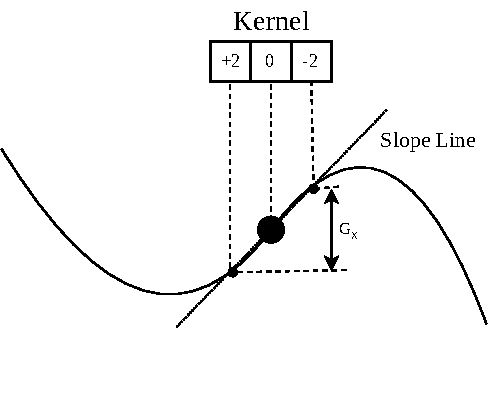
\includegraphics[clip, trim=0 0.25cm 0 0]{slope_score.pdf}
            \caption{Slope Score}
            \label{fig:slope_score}
        \end{figure}

    \subsection{Edge Proximity Score}
    The proximity score aims to bias the selected anchor point away from points near steep inclines in the terrain. This score is defined as the average of the height
    difference of the current point weighted by the gaussian kernel \(\boldsymbol{K}\), of size \(n\) by \(n\). The distance around inclines that is rejected depends on the the
    chosen size of the kernel \(\boldsymbol{K}\), the standard deviation of \(\boldsymbol{K}\) and the height differences. This score is described in Equation
    \ref{eq:terrain_prox}.

    \begin{equation} \label{eq:terrain_prox}
        S_p(x,y) = C_p\left|\frac{\sum\left\langle\boldsymbol{K},(\boldsymbol{h}_{i,j}-\boldsymbol{h}_{x,y})\right\rangle _{\mkern-3mu F}}{n^2}\right|
    \end{equation}

    \noindent
    where,
    \[i = \big[\mkern-4.7mu\big[x- \lfloor\tfrac{1}{2}n\rfloor,\mkern2mu x+\lfloor\tfrac{1}{2}n\rfloor\big]\mkern-4.7mu\big]\]
    \[j = \big[\mkern-4.7mu\big[y-\lfloor\tfrac{1}{2}n\rfloor,\mkern2mu y+ \lfloor\tfrac{1}{2}n\rfloor\big]\mkern-4.7mu\big]\]
    
    
    \noindent
    with \(x\) and \(y\) being the indices of the cell whose score is currently being evaluated, \(\boldsymbol{h}\), the heightmap and \(C_p\) the score's weighting constant.
    
    A diagrammatic, sliced, representation of the proximity score can be seen in Figure \ref{fig:prox_score_diagram}. The
    slice is taken along the x axis of the heightmap.

    \captionsetup[figure]{oneside,margin={0.9cm,0cm}}
    \begin{figure}[h]
        \centering
        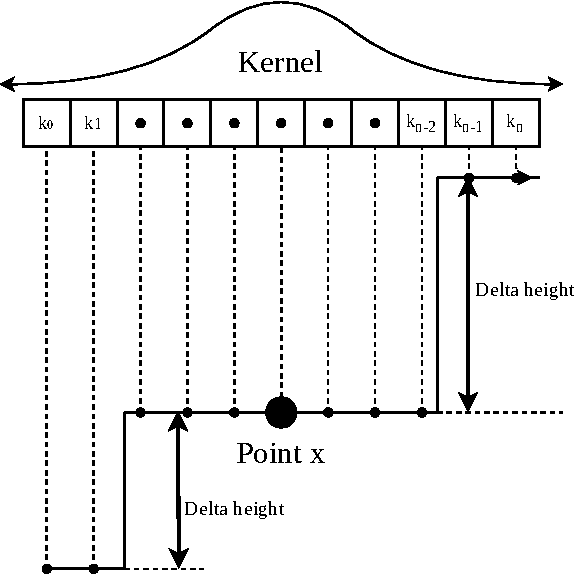
\includegraphics[]{prox_score.pdf}
        \caption{Proximity Score Diagrammatic Representation}
        \label{fig:prox_score_diagram}
    \end{figure}

    \subsection{Constraints}
    It is important to constrain the possible anchor points to conform to the stability triangle, meaning that the centre of mass of the robot must be inside the triangle formed by the three anchor points. Additionally, it is important that the points selected are not too far away, both in the horizontal and vertical direction for the robot to reach.


\section{Score Search Algorithm} \label{sec:radial_search}
    Once the heightmap has been processed into the score map, which is done by adding the
    slope score and terrain proximity score, the point with the best score must be found for every initial anchor point. The resolution of the heightmap is not very high and the adjusted anchor point is not allowed to deviate too far from the initial anchor point. Additionally, due to the parallel nature of the heightmap generation, it is possible to score the entire heightmap with minimal cost. Thus, it was decided to not employ an optimisation algorithm, such as gradient decent or Bayesian, but rather to use a radial search algorithm. This algorithm progressively expands its searching radius over the square score grid until a valid score is found, at which point it
    terminates, thus ensuring that the closest valid point to the initial anchor point is selected. See Figure \ref{fig:radial_search} for a diagram representing the search pattern for a 5 grid squares search area. Note that this search pattern will become inaccurate for large search areas, as the pattern steps in a square manner. This however is not much of a concern for smaller search areas.

    \captionsetup[figure]{oneside,margin={0cm,0cm}}
    \begin{figure}[h]
        \centering
        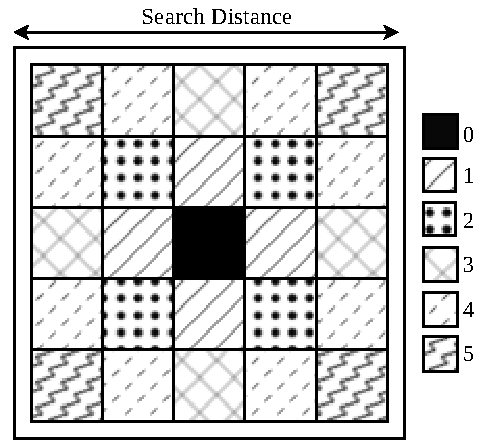
\includegraphics{search_diagram.pdf}
        \caption{Radial search, shown for a 5 cell search diameter.}
        \label{fig:radial_search}
    \end{figure}

    \section{Floor Height Adjustment} \label{sec:height_adjust}
    After the horizontal position of the feet have been optimised, the height of the foot is simply set to the height of the terrain at the target horizontal coordinates. This ensures that the robots body remains level and at a constant global height.

    It is however important to adjust the reference floor height that the robot uses to adapt to a varying average terrain height. If this is not done, then the robot will be incapable of surmounting terrain higher than its commanded standing height, as the robot will simply maintain said height and walk into the tall terrain. There are various methods to choosing a floor height, from using a time of flight sensor underneath the robots main body to using height data from the heightmap.

    The method that was implemented in this project uses the average of the three highest target foot placement positions out of all the robots legs. This allows the robot to pre-emptively increase or decrease its floor height as it targets to step onto higher or lower terrain.

    \captionsetup[figure]{oneside,margin={0cm,0cm}}
    \begin{figure}[h]
        \centering
        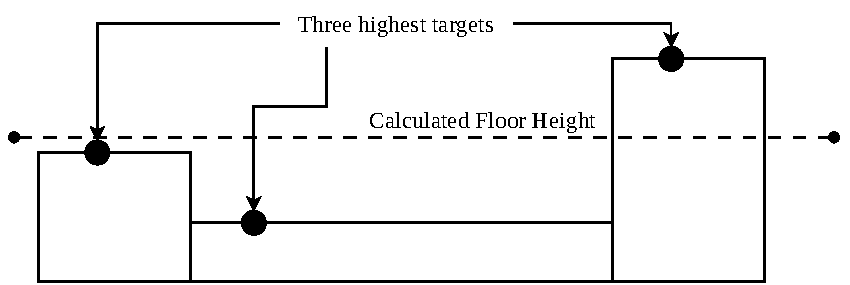
\includegraphics[width=\textwidth]{Diagrams-FloorHeight .drawio.pdf}
        \caption{Floor height diagram.}
        \label{fig:floor_height}
    \end{figure}

    \noindent
    While this method works well to pre-emptively adjust height and to optimise the body height relative to the foot height, it does present one problem: If there is a tall piece of terrain in the path of the robot's body without any feet positioned on it, then the robot will not adjust its body height to clear this piece of terrain. Thus, the bounding box of the robot's body, excluding the legs and feet, is checked against the heightmap. If any point on the heightmap, that is inside the bounding box, is higher than the previously set floor height, the floor height is updated to this increased height.

    \newpage
    \section{Scoring Test on Simulated Terrain} \label{sec:test_scores}
    For testing the walkability scores described in section \ref{sec:scores}, a piece of terrain that demonstrates various types of obstacles that the robot might encounter was simulated. This terrain and its heightmap is shown in figure \ref{fig:score_test_map}.
    \begin{figure}[h]
        \centering
        \begin{subfigure}{.5\textwidth}
            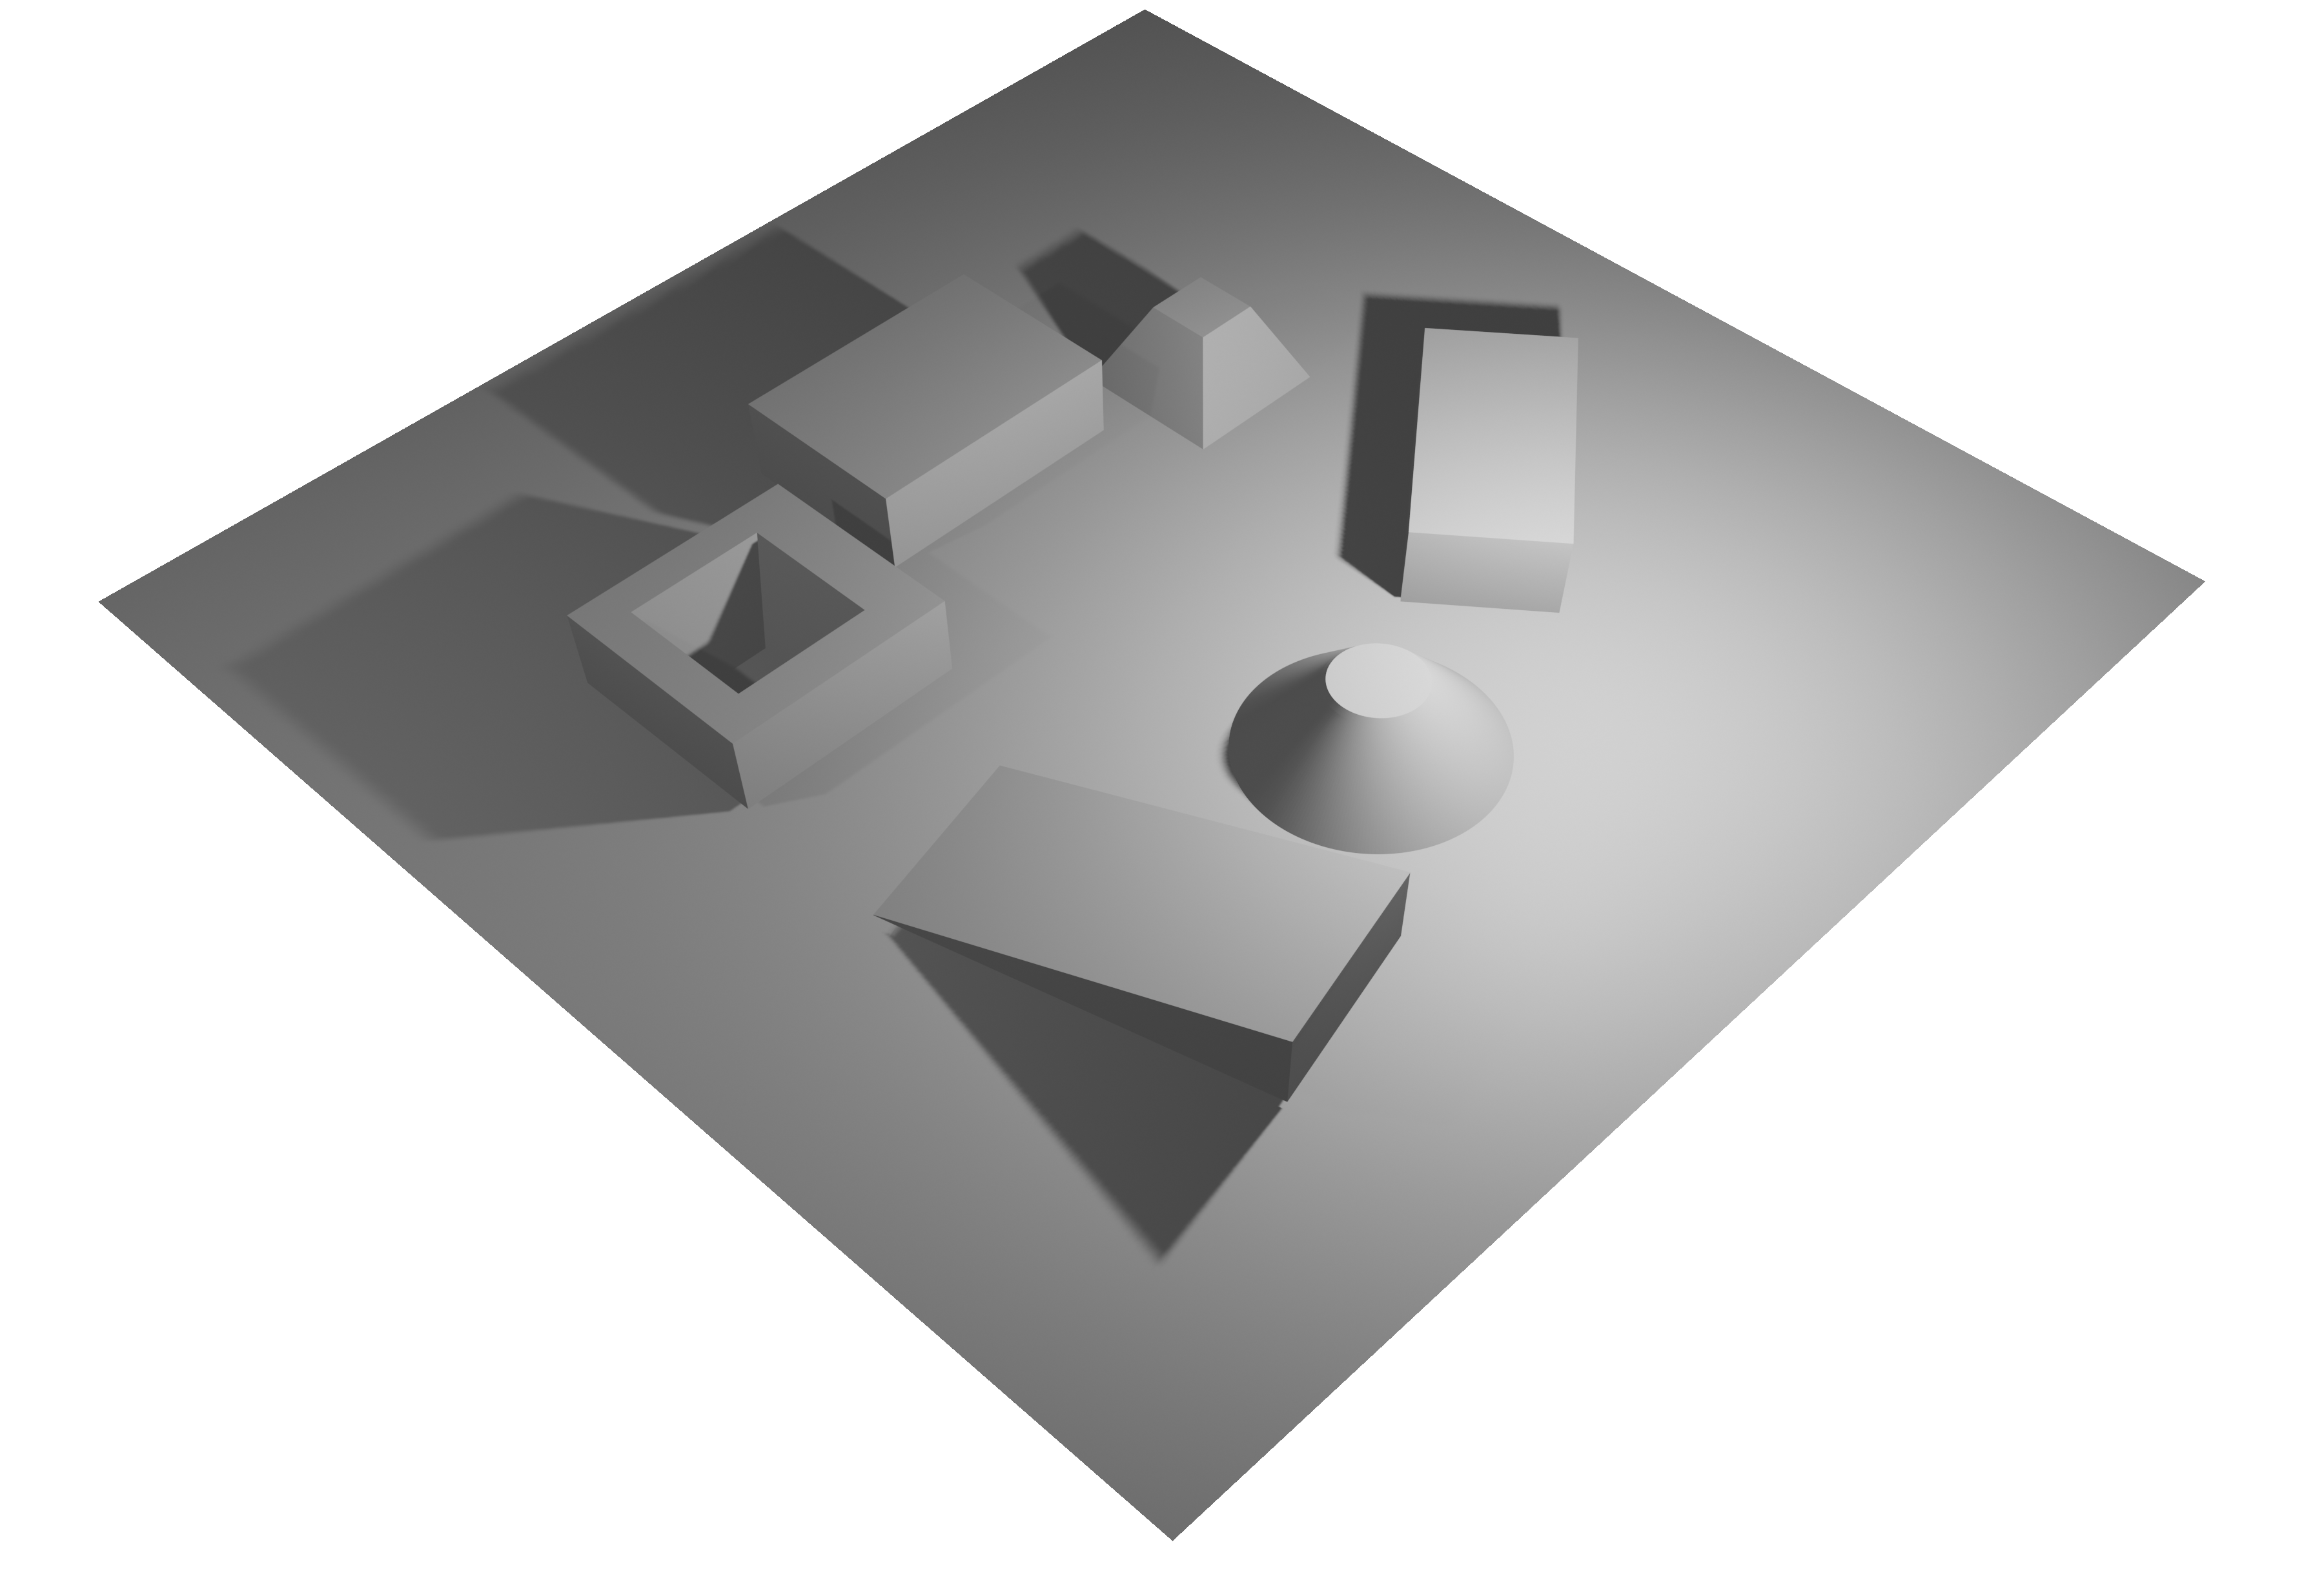
\includegraphics[height=.8\linewidth, left]{hmap3D.png}
            \caption{3D Terrain}
            \label{fig:sub_3d_terrain}
        \end{subfigure}%
        \begin{subfigure}{.5\textwidth}
            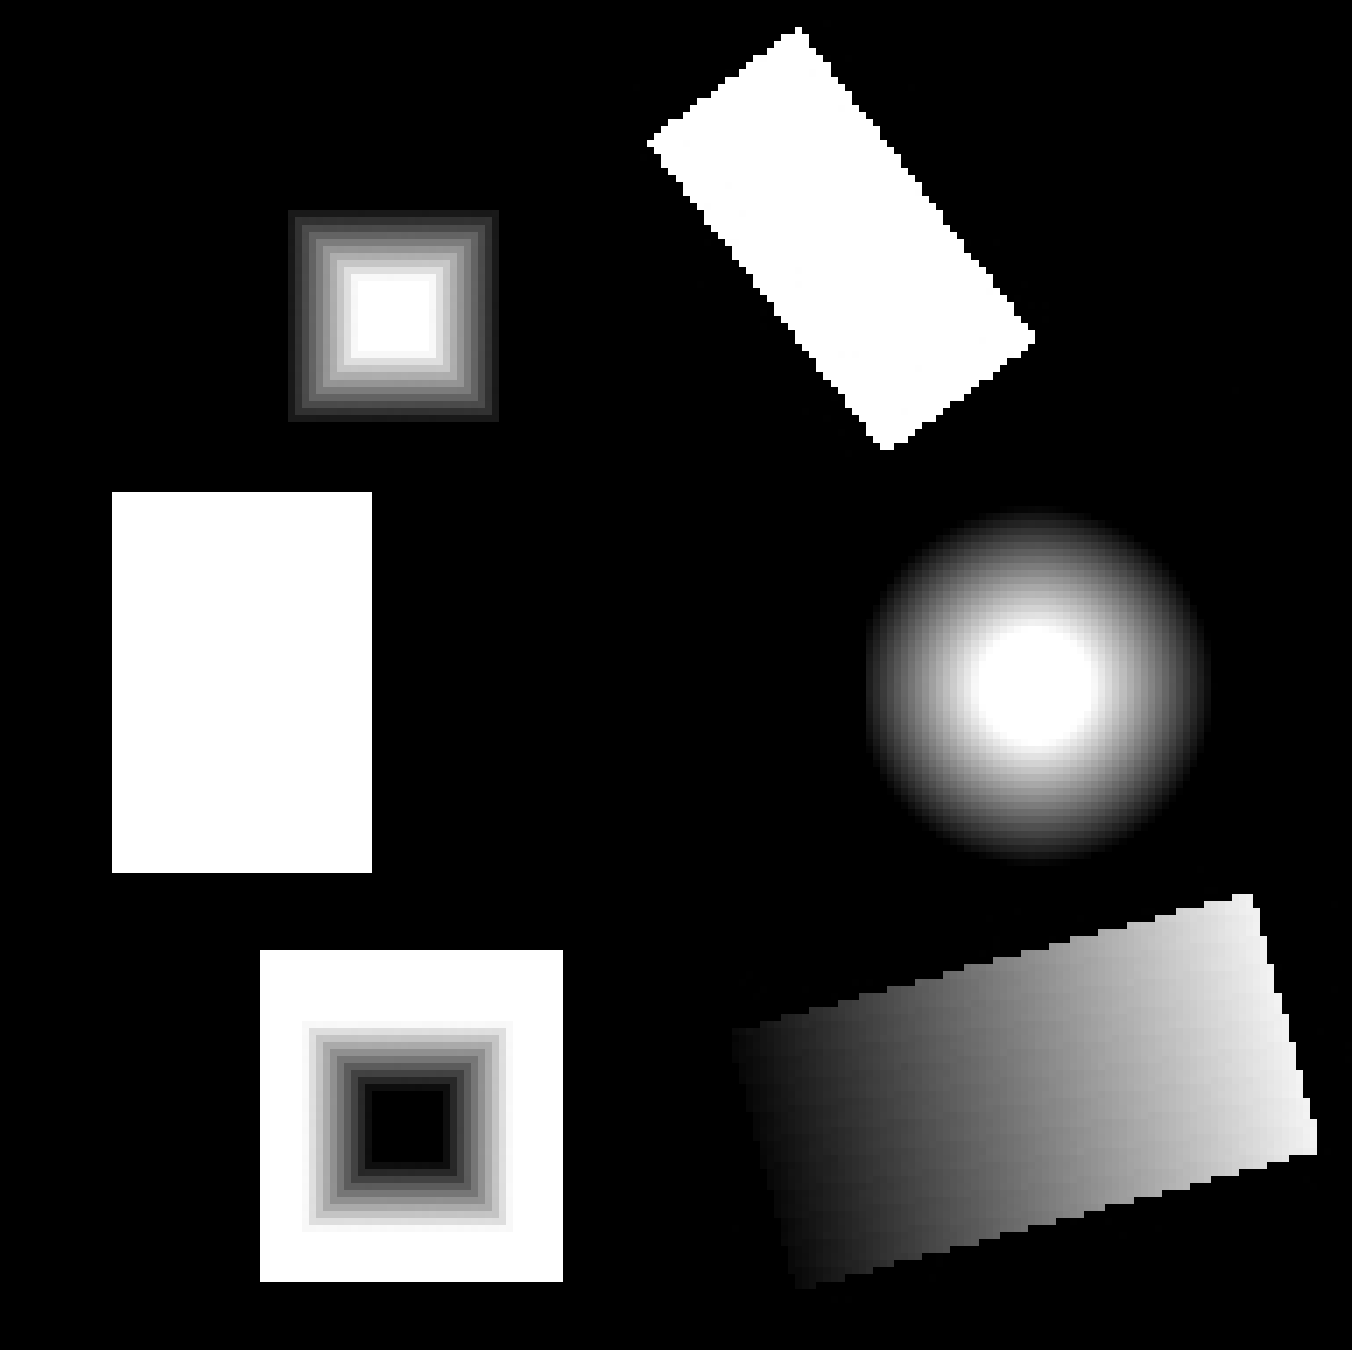
\includegraphics[height=.8\linewidth, right]{scoreTestHmap.png}
            \caption{Heightmap of 3D Terrain}
            \label{fig:sub_3d_terrain_hmap}
        \end{subfigure}
        \caption{3D Model of Terrain and its heightmap.}
        \label{fig:score_test_map}
    \end{figure}

    \noindent
    The heightmap in figure \ref{fig:sub_3d_terrain_hmap} is used to test the various walkability scores. First, in order to show individual results, the slope and edge proximity scores are applied to the heightmap separately. This is shown in figure \ref{fig:scores_seperate}. Next the combined score is shown in figure \ref{fig:full_score}. This is the score that is used to optimise foot end positions.
    \begin{figure}[h]
        \centering
        \begin{subfigure}{.45\textwidth}
            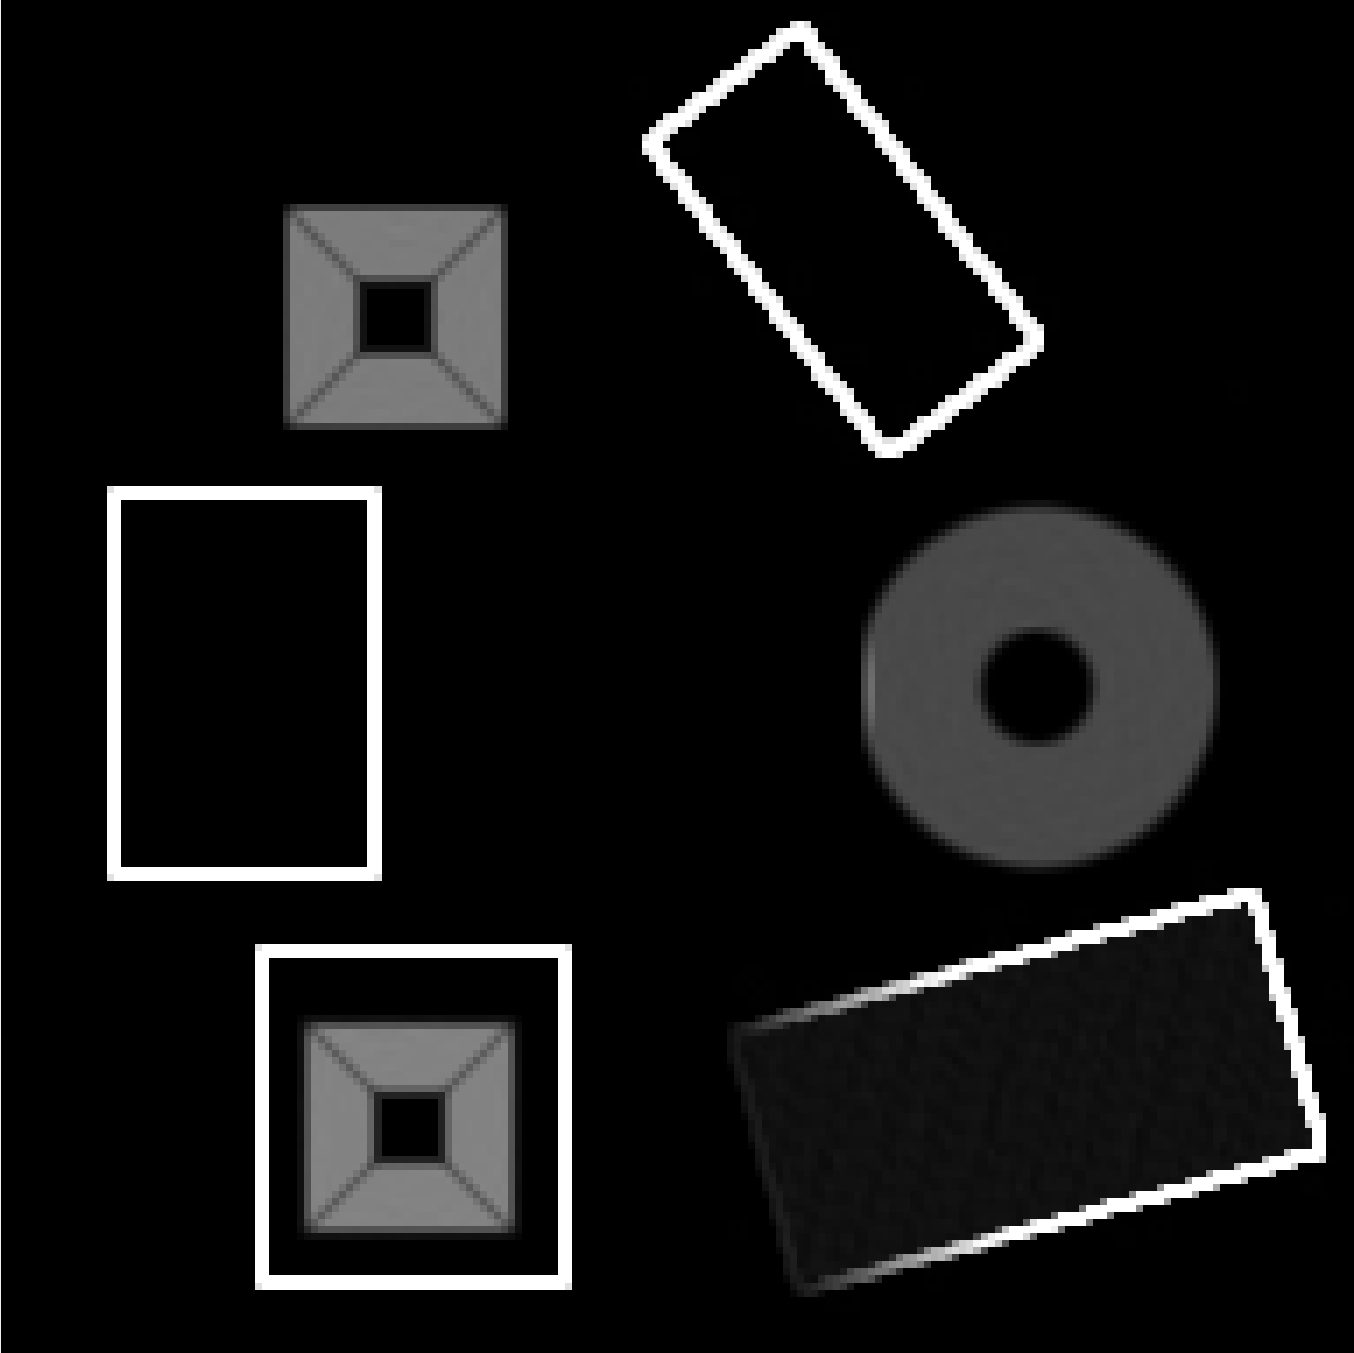
\includegraphics[height=.85\linewidth, left]{slopeScoreTest.png}
            \caption{Slope score test.}
            \label{fig:sub_slope_test}
        \end{subfigure}%
        \begin{subfigure}{.45\textwidth}
            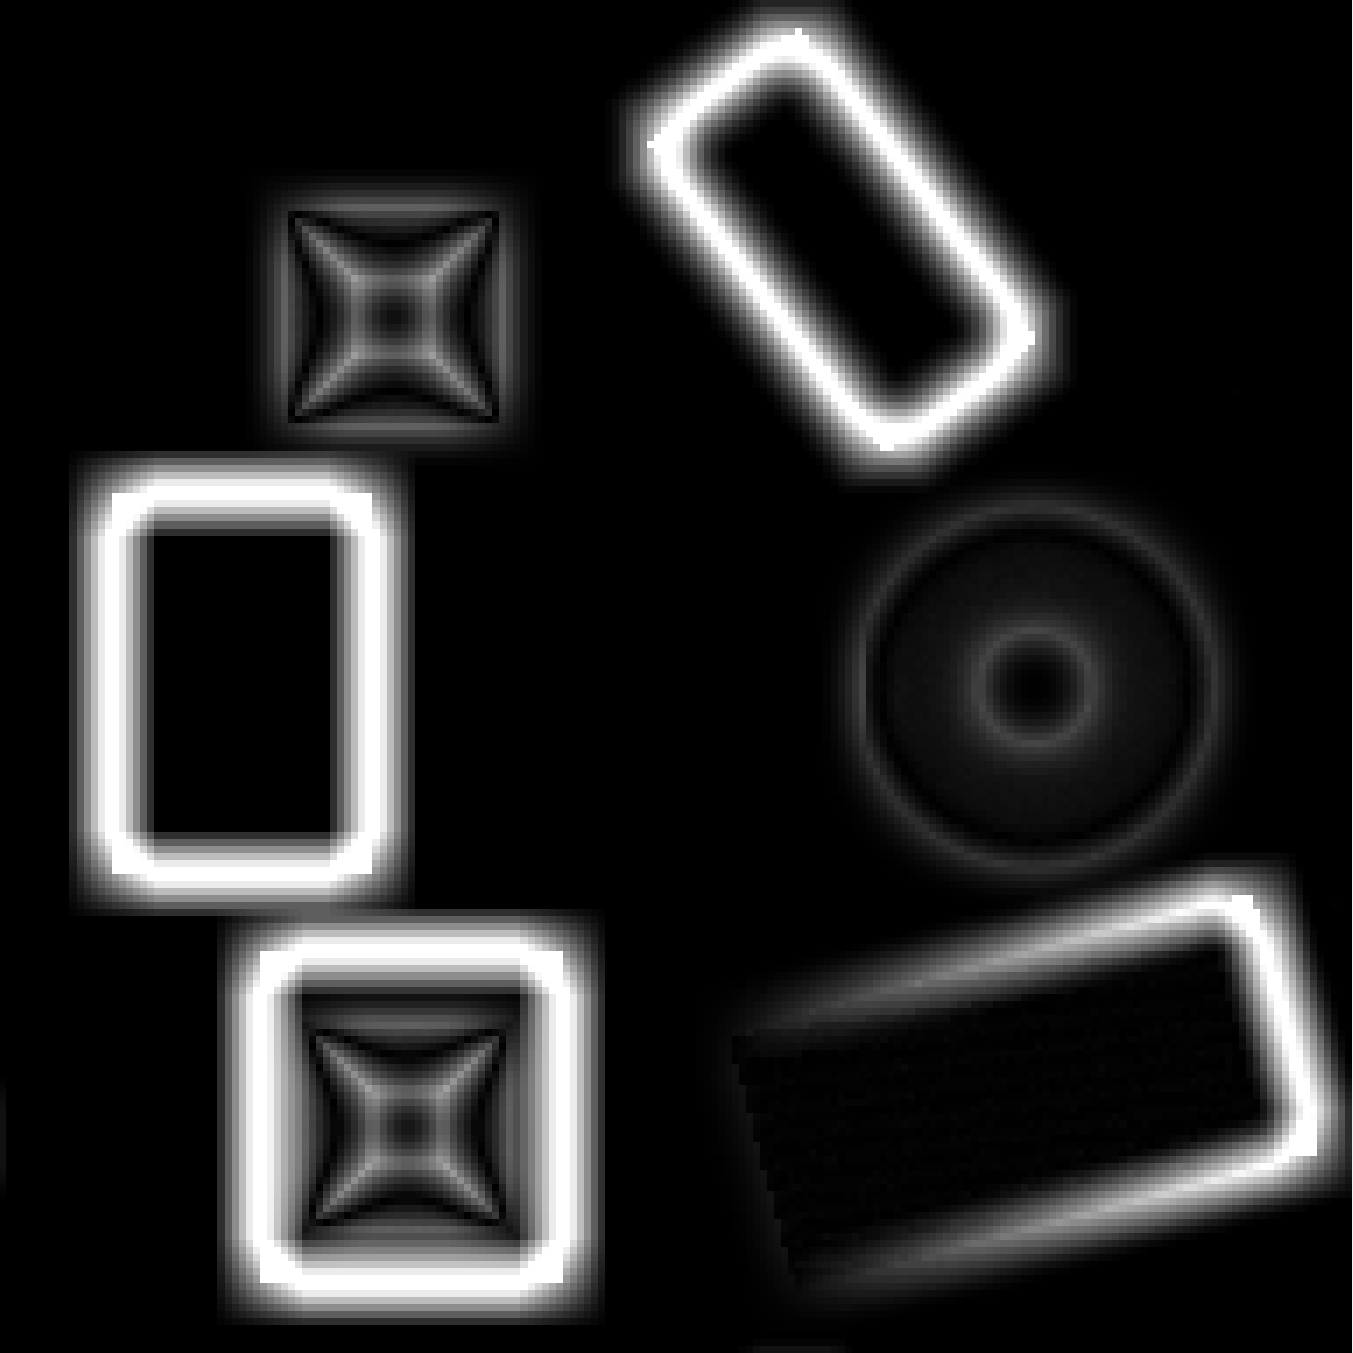
\includegraphics[height=.85\linewidth, right]{proxScoreTest.png}
            \caption{Edge proximity score test.}
            \label{fig:sub_prox_test}
        \end{subfigure}
        \caption{Slope score and edge proximity score tests.}
        \label{fig:scores_seperate}
    \end{figure}
    The score images show a gradient from black to white, darker colours indicate more desirable foot placement positions, while light colors indicate undesirable locations.

    The slope score can be seen in figure \ref{fig:sub_slope_test}. From this it can be seen that the slope score successfully indicates sloped areas
    as less suitable foot end positions. It is also clear that vertical inclines are strongly discouraged, and while not the primary purpose of the slope
    score, this is expected and does not have a negative impact on scoring.

    Figure \ref{fig:sub_prox_test} shows that edge proximity score successfully discourages foot placement in areas with large height deviations,
    while allowing placement in areas with a locally similar slope, such as the ramp in the bottom-right. As can be seen from the larger, and more intense, discourage areas around the boxes in the
    top-right, bottom-right, left and bottom-left, it is clear that the magnitude of the height differential will increase the size and strength of the rejection area.
    Next, in figure \ref{fig:full_score} the combined slope and edge proximity scores can be seen. This is simply the sum of the two scores.
    \begin{figure}[h]
        \centering
        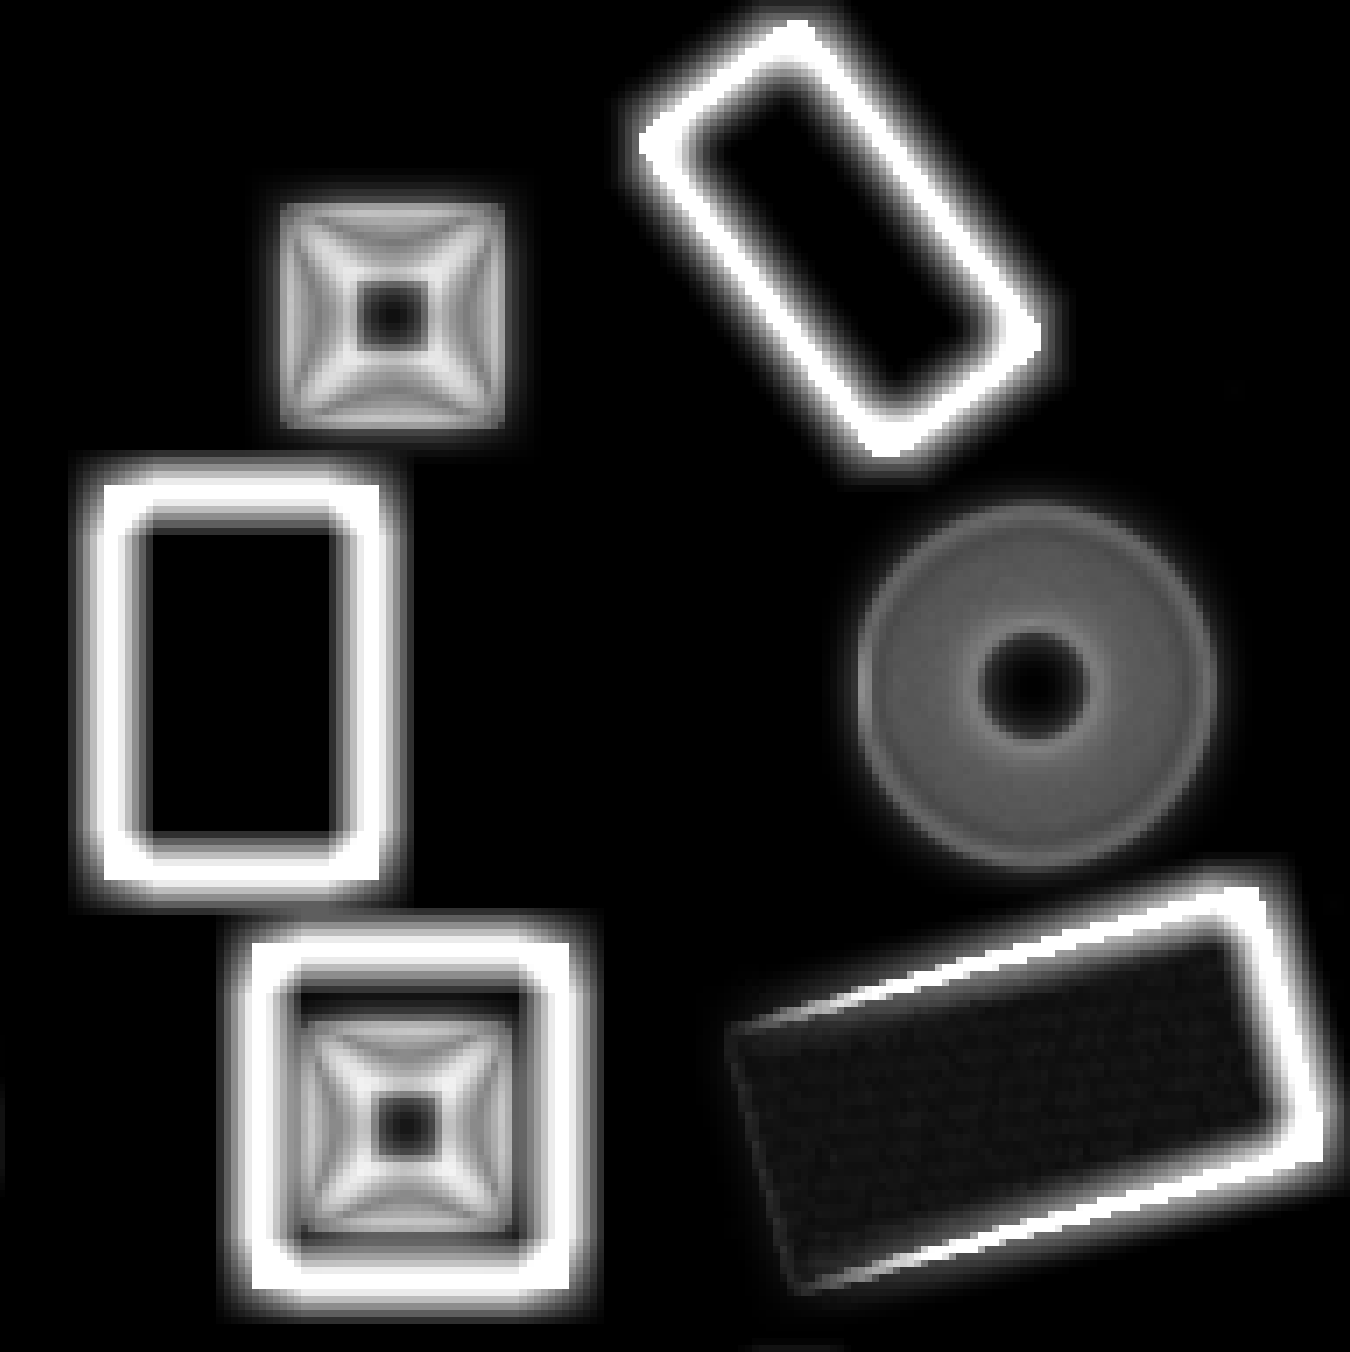
\includegraphics[width=.49\textwidth]{fullScore.png}
        \caption{Full walkability score.}
        \label{fig:full_score}
    \end{figure}

    \noindent
    Finally, the radial search algorithm described in section \ref{sec:radial_search} is used to optimise various nominal foot end positions. This is shown in figure \ref{fig:optimisation_test}. In this figure the blue box indicates the search area of the radial search algorithm from section \ref{sec:radial_search}. The red marker indicates the nominal foot position that would be received from the baseline motion system, and the green marker is the walkability score optimised foot position. If there is only a green marker this means that the nominal position was already valid, and no adjustment is necessary.
    \newpage
    \begin{figure}[h]
        \centering
        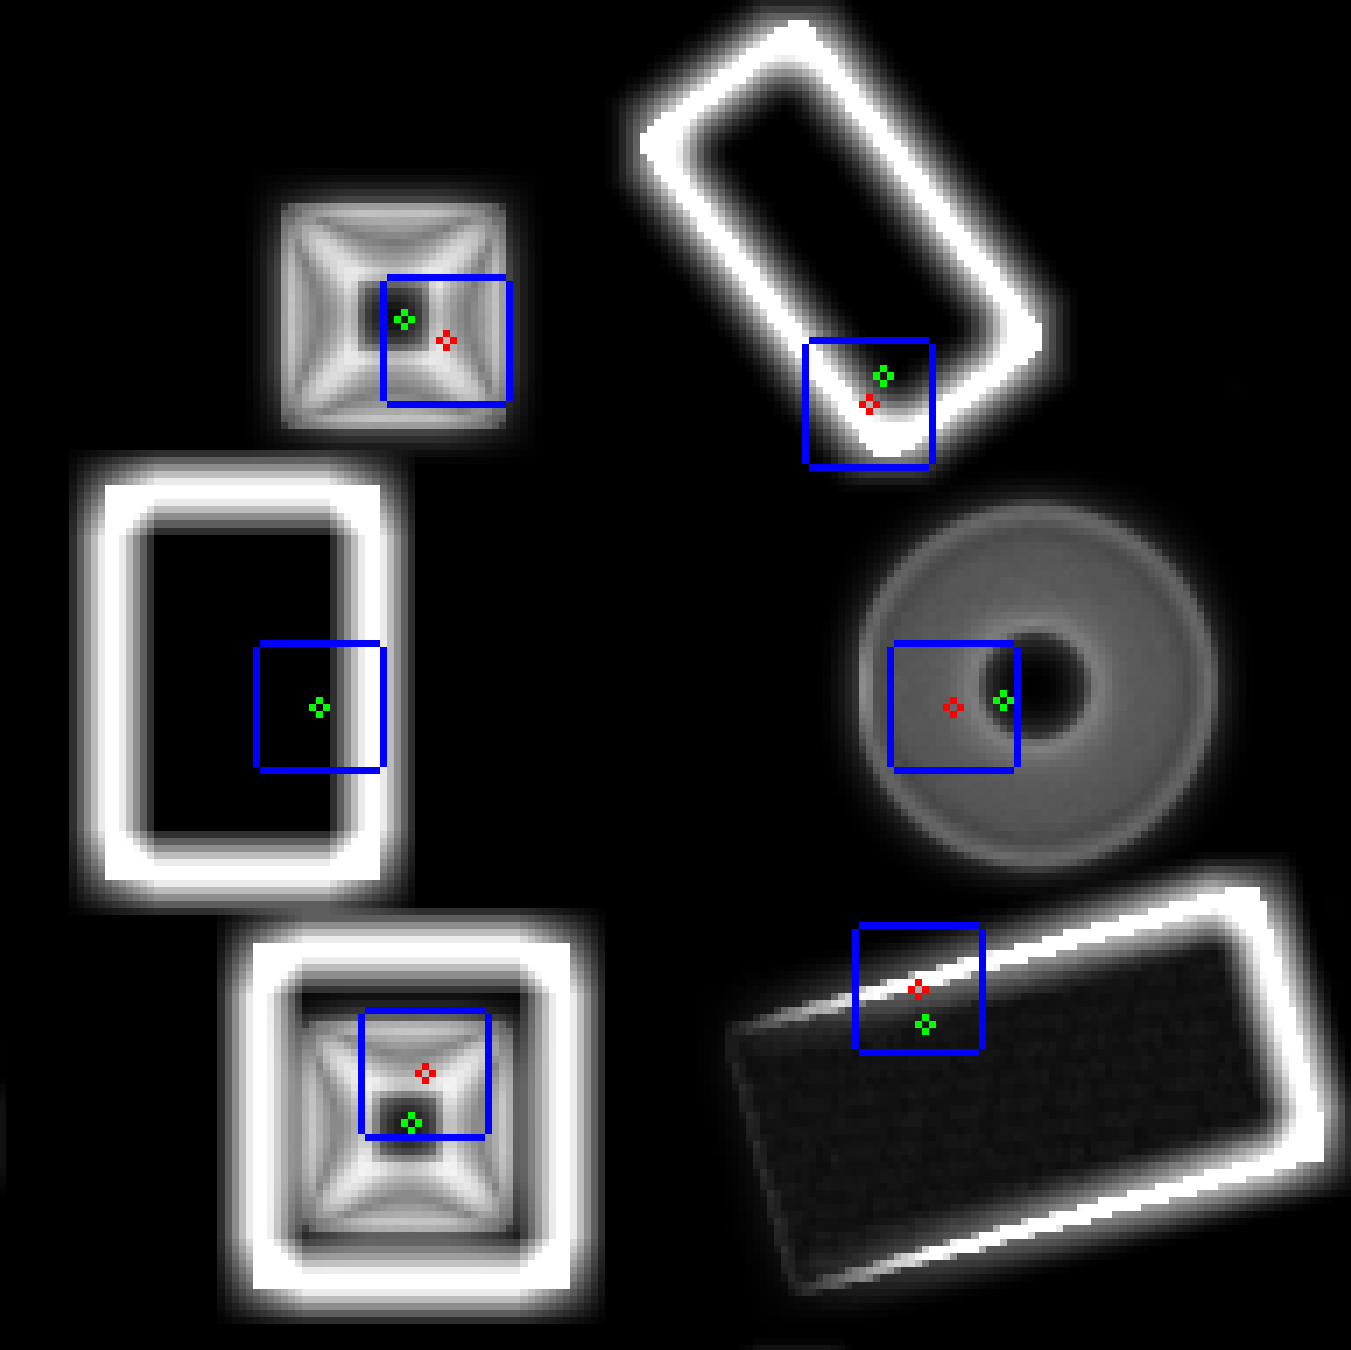
\includegraphics[width=.6\textwidth]{scoreTestFinal.png}
        \caption{Walkability score optimisation test.}
        \label{fig:optimisation_test}
    \end{figure}

    \noindent
    If the nominal foot position has an acceptable score, the position will not be adjusted. This can be seen with the middle-left nominal foot placement position in figure \ref{fig:optimisation_test} where the green marker coincides with the red marker. If however the nominal placement position is too close to an edge, such as with the top-right example, the nominal position is adjusted to the closest acceptable position. The adjusted position does not need to have a perfect score, as illustrated by the bottom-right example. This example is similar to the top-right example, with the nominal foot placement located too close to an edge. However, it adjusts the foot placement onto the ramp, which has a non-zero, but acceptable, walkability score. Next, the middle-right example shows how the nominal placement position is placed on a piece of terrain that is too steep. Thus, it is adjusted onto the flat surface on top of the round pedestal. 
    
    % \noindent
    Finally, the top-left and bottom-left examples show the cases of nominal foot placement positions placed on a sloped pillar and a sloped hole, respectively. In both cases the nominal placements are adjusted to the flat surface at the top of the pillar and at the bottom of the hole respectively. (The foot could be placed at the bottom of the hole, because the height there is known.).
    
    The flat surfaces on the pillar an in the hole are large enough not to be rejected by the edge proximity score. However, if the slopes were steeper or the flat surfaces were smaller, these nominal positions could be unsolvable, as there would be no suitable foot placement positions inside the search area. In this case the robot would need to make a course adjustment.

    \newpage
    \section{Scoring Test on Physical Terrain}
        The walkability scoring system was also tested on the practical heightmap that was generated from real RGB-D images recorded by the physical hexapod. Using the same colour scheme as above, the practical heightmap found in section \ref{sec:hardware_hmap} is again shown for reference in figure \ref{fig:harware_hmap}. The scoring system was then applied to this heightmap and the resulting walkability score map is shown in figure \ref{fig:hardware_score_map}.
        \begin{figure}[h]
            \centering
            \begin{subfigure}{.45\textwidth}
                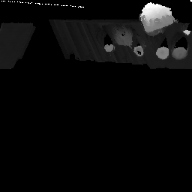
\includegraphics[height=.95\linewidth, left]{hardware_map.png}
                \caption{Hardware heightmap}
                \label{fig:harware_hmap}
            \end{subfigure}%
            \begin{subfigure}{.45\textwidth}
                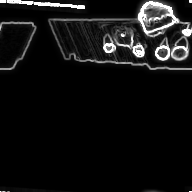
\includegraphics[height=.95\linewidth, right]{score_test_hardware.png}
                \caption{Score applied to hardware heightmap.}
                \label{fig:hardware_score_map}
            \end{subfigure}
            \caption{Heightmap generated from hardware and the corresponding score map.}
            \label{fig:hardware_hmap_scoremap}
        \end{figure}

        \noindent
        As can be seen from figure \ref{fig:hardware_hmap_scoremap} the scoring system applied to the hardware-generated heightmap functions similarly to when it is applied to a simulated heightmap. The primary difference that should be noted is the score artifacts created around the mapped areas edge, seen as an outline around the mapped area. Light score lines can also be seen as diagonal stripes within the mapped area. These lines are most clear on the portion of flat terrain. The lines are created by the moving field of vision and inaccuracies in the pose estimate obtained from ORB-SLAM3, mostly inaccuracies in the height estimates, as explained previously in section \ref{sec:hardware_hmap}.

        It should also be noted that, while the score for the sloped plane at the top of the heightmap is not as even as it was in the ideal heightmap, even with these undulations present it is still sufficiently accurate for the correct foot position adjustment to be made. This can be seen in figure \ref{fig:hardware_test_points} which shows how different hypothetical nominal foot placement positions would be adjusted based on the hardware-generated score map.

        \newpage
        \begin{figure}[h]
            \centering
            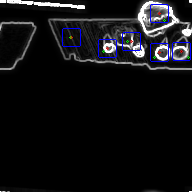
\includegraphics[width=.6\textwidth]{score_test_hardware_points.png}
            \caption{Test points on hardware score map.}
            \label{fig:hardware_test_points}
        \end{figure}

        \noindent
        The results show that all of the nominal foot placements are adjusted to suitable new placement positions, where necessary. Note the point applied to the sloped plane at the top of the map is adjusted appropriately even with the slightly undulating score map across the sloped area.

        Additionally, it should be noted that while some of the outlining artifacts do grow large enough to affect the final foot positions, as can be seen in the
        left most test point, these effects are generally not large enough to be of  concern.


% \bigskip
% \bigskip
% \hrule
% \smallbreak
% \hrule
\chapter{Hardware Implementation} \label{chap:hardware}
This chapter describes the practical implementation of the system on the physical hexapod robot. Section  \ref{sec:hardware_overview} provides an overview of the implementation. Section \ref{sec:ros_nodes} describes the \ac{ros} in the system, their functions and the data they communicate. Appendix \ref{app:ros_comms} describes the details of the \ac{ros} messages sent by the nodes and their data types.

\section{Overview} \label{sec:hardware_overview}
The entire system was implemented in the \acf{ros} environment, \ac{ros} is a system which, among other things, greatly simplifies the task of communication between devices using various different communication protocols. This is achieved by sectioning all code into different \ac{ros} nodes, where every node is treated as a component in a large network. All ros nodes are joined together by the core node, which is hosted at a set IP address on the network.

\newpage
\section{ROS Architecture} \label{sec:ros_nodes}
    The various \ac{ros} nodes are distributed between the base station on the desktop computer, and the Jetson Nano and the Teensy \ac{mcu} on the hexapod robot. Figure \ref{fig:nodes} provides an overview of the nodes and how they communicate with each other.

    \captionsetup[figure]{oneside,margin={0cm,0cm}}
    \begin{figure}[h]
        \centering
        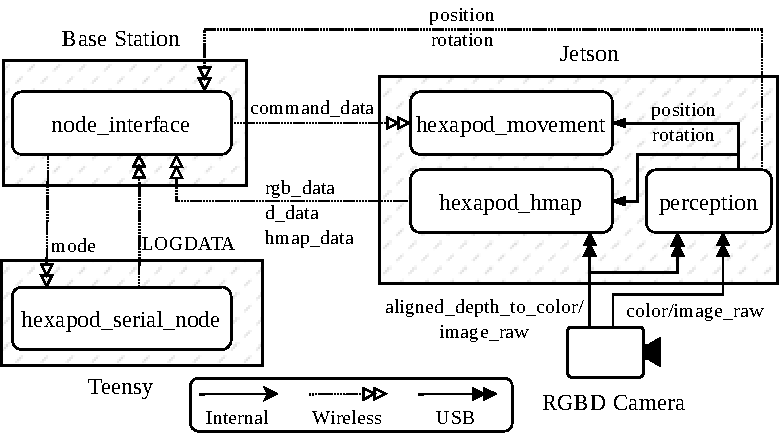
\includegraphics{Diagrams-Nodes.drawio.pdf}
        \caption{ROS nodes and communication.}
        \label{fig:nodes}
    \end{figure}

    \noindent
    Note that the data transfer arrows between the base station and the teensy are a combination of the wireless and USB arrows, this implies that the data passes to the Jetson as a intermediate step. Transfers between the base station and the Jetson are wireless, while between the Jetson and the Teensy are through USB. Section \ref{sec:base_ros} and \ref{sec:on_board_ros} provide details on the node architecture shown in figure \ref{fig:nodes}.
    \subsection{Base Station} \label{sec:base_ros}
        The base station consists of a single \ac{ros} node, this node is responsible for transmitting all commands to and receiving data from the robot. The base station publishes two messages, the mode message and the command data message. As the names imply the mode message contains the commanded mode that the robot should switch to, while the command data message contains the remaining commands that the operator could issue. The mode is separated from the other commands because it is only sent to the Teensy, while the other commands are sent to the Jetson.
        
        The base station subscribes to the pose message from the perception node, and the rgb data, d data and hmap data from the hexapod map node, and also the LOGDATA message from the hexapod serial node. The pose message contains the pose estimate produced from ORB-SLAM3, while the rgb data, d data and hmap data message contain the color, depth and heightmap images respectively. The LOGDATA message contains generic string log messages from the Teensy.
        
        The base station is what the operator uses to observe and issue commands to the robot, as such there is wireless communication link between the robot and the base station.
        % For a description of the base station publishers see table \ref{tab:base_pubs} and for its subscribers see \ref{tab:base_subs}. Table \ref{tab:data_types} describes
        % data types used.
        % \begin{table}[h]
        %     \centering
        %     \begin{tabularx}{\textwidth}{| l | l | X | l |}
        %         \hline
        %         \multicolumn{4}{|c|}{\textbf{Base Station Publishers}} \\ \hline
        %         \textbf{Name} & \textbf{Data Type} & \textbf{Description} & \textbf{Frequency} \\ \hline
        %         % walk\_dir & Description & Data Type & Frequency \\ \hline
        %         command\_data & HexapodCommands & Various robot command parameters. & On change \\ \hline
        %         mode & Int32 & Specifies the oporationg mode of the robot. & On change. \\ \hline
        %     \end{tabularx}
        %     \caption{Base station publishers}
        %     \label{tab:base_pubs}
        % \end{table}
        Among the commands the operator can send the robot is the operating mode, the robot currently only has two operating modes, torque cutoff mode and walking mode. The torque cutoff mode is the initial mode the robot is in, while in this mode the leg servos disable all torque control, thus entering a relaxed state. In walking mode the robot walks in the commanded direction whilst optimising its foot positions according to the terrain. If the robot encounters a piece of terrain for which no optimisation can be found the human controller will have to adjust the walking direction from the base station.

        % \begin{table}[h]
        %     \centering
        %     \begin{tabularx}{\textwidth}{| l | l | X |}
        %         \hline
        %         \multicolumn{3}{|c|}{\textbf{Base Station Subscribers}} \\ \hline
        %         \textbf{Name} & \textbf{Data Type} & \textbf{Description} \\ \hline
        %         % walk\_dir & Description & Data Type & Frequency \\ \hline
        %         rgb\_data & Image & The processed color image from the robot. \\ \hline
        %         d\_data & Image & The processed color depth from the robot. \\ \hline
        %         hmap\_data & Image & The heightmap generated on the robot. \\ \hline
        %         LOGDATA & String & General logs from the robot. \\ \hline
        %     \end{tabularx}
        %     \caption{Base station subscribers}
        %     \label{tab:base_subs}
        % \end{table}
        
        % \noindent
        % The only subscribers present on the base station are the processed camera images, heightmap and logs. These are all used to provide a interface from where
        % the operator can control the robot.

    \subsection{On Board} \label{sec:on_board_ros}
        The hexapod has two computational units on board, first the Jetson Nano, which handles all high level operations, including heightmap generation and scoring, foot optimisation, maintain a walking gait and localisation using ORB-SLAM3. Secondly a Teensy2.0 \ac{mcu} handles low level operations, including interpolating feet movement paths and servo control.

        The Jetson hosts four different nodes, the hexapod hmap, hexapod movement, RGBDSLAM and rs camera nodes. The rs camera node publishes the camera stream consisting of the color and aligned depth to color messages. As could be deduced from the names, the depth message is aligned to the color. These messages are transmitted at a rate of 30Hz.
        
        The RGBDSLAM module runs the ORB-SLAM3 algorithm and subscribes to the depth and color streams from the rs camera node as inputs. As ORB-SLAM3 uses both the color and depth streams for pose estimation these streams are synchronised in time. Once the pose is estimated it is published in the pose message.

        The hexapod hmap node is responsible for generating the heightmap and score maps. It subscribes to the pose, depth and color messages, the depth and color messages are downsampled before being used to generate the heightmap. The entire generation process is ran on the Jetson Nano's \ac{gpu} as described in chapter \ref{chap:mapping}. Once the heightmap and scoremap are generated they are published in the hmap data and scoremap data messages. Additionally the downsampled colour and depth messages are also published for transmission to the base station.

        Next the hexapod movement node subscribes to the command, pose, hmap and scoremap messages to generate and optimise the feet targets, as described in chapter \ref{chap:motion} and \ref{chap:optimisation}. The feet targets are published as the effector targets message.

        Lastly, the Teensy \ac{mcu} also consists of a single \ac{ros} node, the hexapod serial node. The functionality of this node is simply to facilitate communication over USB. The node is subscribed to the mode and effector targets messages, these messages are then used to calculate the feet trajectories as described in chapter \ref{chap:motion}. The trajectories are then translated into servo angles and angular rates, also described in chapter \ref{chap:motion}. Whereafter the servos are actuated. The only publisher present on the Teensy is the LOGDATA publisher, which simply publishes general string log messages for use by the operator.
    %     Table \ref{tab:jetson_pubs} to \ref{tab:teensy_subs} describe the \ac{ros} publishers and subscribers present on these two computational units.
        
    %     The camera data, heightmap data, position and rotation are published for display at the base station.
    %     While the effector targets are published for use on the Teensy to move the robot's feet to the optimised positions.
    %     \newpage
    %     \begin{table}[h]
    %         \centering
    %         \begin{tabularx}{\textwidth}{| l | l | X | l |}
    %             \hline
    %             \multicolumn{4}{|c|}{\textbf{Jetson Publishers}} \\ \hline
    %             \textbf{Name} & \textbf{Data Type} & \textbf{Description} & \textbf{Frequency} \\ \hline
    %             % walk\_dir & Description & Data Type & Frequency \\ \hline
    %             effector\_targets & EffectorTargets & Data indicating which feet to move where, and what type of interpolation to use. & On change\\ \hline
    %             rgb\_data & Image & The processed color image from the \ac{rgbd} camera. & 15Hz. \\ \hline
    %             d\_data & Image & The processed depth image from the \ac{rgbd} camera. & 15Hz. \\ \hline
    %             hmap\_data & Image & The heightmap generated on the robot. & 15Hz. \\ \hline
    %             position & Vector3 & The localised position of the robot & 15Hz \\ \hline
    %             rotation & Quat & The localised rotation of the robot & 15Hz \\ \hline
    %         \end{tabularx}
    %         \caption{Jetson publishers}
    %         \label{tab:jetson_pubs}
    %     \end{table}
    %     % \newpage
    %     \begin{table}[h]
    %         \centering
    %         \begin{tabularx}{\textwidth}{| l | l | X |}
    %             \hline
    %             \multicolumn{3}{|c|}{\textbf{Jetson Subscribers}} \\ \hline
    %             \textbf{Name}  & \textbf{Data Type} & \textbf{Description} \\ \hline
    %             % walk\_dir & Description & Data Type & Frequency \\ \hline
    %             command\_data & HexapodCommands & Operator commands. \\ \hline
    %             color/image\_raw & Image & Color image from the camera. \\ \hline
    %             aligned\_depth\_to\_color/image\_raw & Image & Depth image from the camera. \\ \hline
    %         \end{tabularx}
    %         \caption{Jetson subscribers}
    %         \label{tab:jetson_subs}
    %     \end{table}

    %     As can be seen from table \ref{tab:jetson_subs} the only subscribers required on the Jetson is the raw camera feed, 
    %     for constructing the heightmap, and the commands from the base station.

    %     Table \ref{tab:teensy_pubs} show that the Teensy publishes the current feet positions these are the positions calculated through \ac{fk}. Additionally
    %     log data is also published for use on the base station.
    %     \begin{table}[h]
    %         \begin{tabularx}{\textwidth}{| l | l | X | l |}
    %             \hline
    %             \multicolumn{4}{|c|}{\textbf{Teensy Publishers}} \\ \hline
    %             \textbf{Name} & \textbf{Data Type} & \textbf{Description} & \textbf{Frequency} \\ \hline
    %             LOGDATA & String & General logs. & 10Hz \\ \hline
    %             effector\_current\_position & Eigen::Vector3d & Current feet positions. & 10Hz \\ \hline
    %         \end{tabularx}
    %         \caption{Teensy publishers}
    %         \label{tab:teensy_pubs}
    %     \end{table}
    %     \begin{table}[h]
    %         \centering
    %         \begin{tabularx}{\textwidth}{| l | l | X |}
    %             \hline
    %             \multicolumn{3}{|c|}{\textbf{Teensy subscribers}} \\ \hline
    %             \textbf{Name} & \textbf{Data Type} & \textbf{Description} \\ \hline
    %             % walk\_dir & Description & Data Type & Frequency \\ \hline
    %             command\_data & HexapodCommands & The color image from the \ac{rgbd} camera. \\ \hline
    %             effector\_targets & EffectorTargets & Data indicating which feet to move where, and what type of interpolation to use.\\ \hline
    %             mode & Int32 & Receives mode data from the base station \\ \hline
    %         \end{tabularx}
    %         \caption{Teensy subscribers}
    %         \label{tab:teensy_subs}
    %     \end{table}

    %     Lastly, from table \ref{tab:teensy_subs} it can be seen that the Teensy subscribes to the command data, effector targets and mode.
    %     The walking speed component from the command data is used to set the rotational rate of the servos, as discussed in section \ref{sec:ang_rate}.
    %     The effector targets are used to interpolate a curve for the feet to move along, as described in section \ref{sec:arc_generation}. The mode is required
    %     as some modes could integrate directly with the servo control, namely the torque cutoff mode.

    % \newpage
    % \subsection{ROS Data Types}
    %     Various custom \ac{ros} data types are defined to assist with communication, these data types are described in table \ref{tab:data_types}.
    %     \begin{table}[h]
    %         \centering
    %         \begin{tabularx}{\textwidth}{| l | p{\widthof{float32\([2]\) walk\_dir}} | X |}
    %             \hline
    %             \textbf{Name} & \textbf{Type Definition} & \textbf{Description} \\ \hline
    %             % walk\_dir & Description & Data Type & Frequency \\ \hline
    %             Vector3 & float\([3]\) data. & A vector in 3D space.  \\
    %             \hline
    %             EffectorTargets & Vector3\([6]\) targets \newline 
    %                             bool\([6]\) swinging. & Data describing the targets of the robot's feet and which feet are swinging. \\
    %             \hline
    %             HexapodCommands & float32\([2]\) walk\_dir \newline
    %                             float32 speed \newline
    %                             float32 height & Data packet containing various command parameters for the robot. \\
    %             \hline
    %         \end{tabularx}
    %         \caption{\ac{ros} data type descriptions}
    %         \label{tab:data_types}
    %     \end{table}
\chapter{Final Walking Tests}
    The final walking tests are comprised of three different terrains: a simple flat plane as a baseline, then a staircase to demonstrate simple foot and body height adjustment, and finally a uneven organic like surface.

    Please note that all data is plotted with the world axis aligned to the robot's starting orientation in the world. This is done for graphing clarity.
    
    % When presenting testing data, a snapshot of the 3D simulation environment will be shown, with the body and foot paths traced. Additionally key data points
    % are also graphed, however only the height of a single foot will be graphed, this is to maintain clarity.

    \section{Flat Terrain}
    The flat plane test aims to quantify nominal body height oscillations and to provide a baseline to compare subsequent test to. Figure \ref{fig:plane_test} and \ref{fig:plane_test_top} shows screenshots of the simulation test being performed in \ac{mujoco}. A video of the simulation can be seen \href{https://youtu.be/pw4GzVp-8aQ}{\underline{here}}.
    \begin{figure}[h]
        \centering
        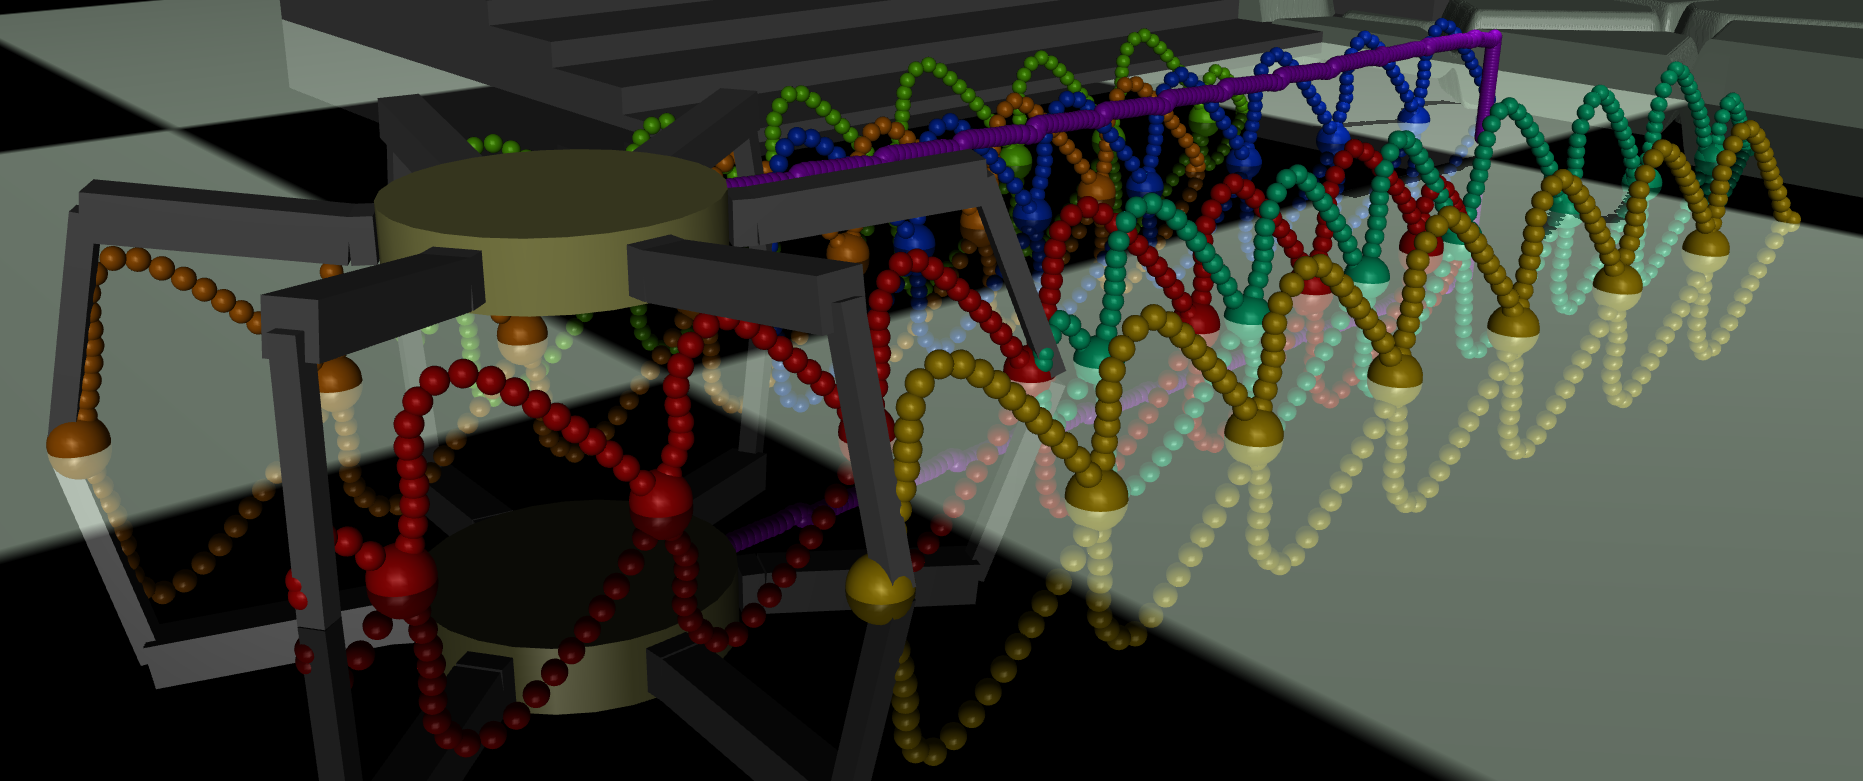
\includegraphics[width=\textwidth]{Flat.png}
        \caption{Flat terrain \ac{mujoco} view.}
        \label{fig:plane_test}
    \end{figure}

    \noindent
    The test was performed with a nominal stride length of 15cm, while the flow function parameters \(Ch\) and \(q\) were set to 2.0 and 14.0 respectively. This equates to a desired step height roughly equal to true stride length, which is dependant on the terrain. The target body height was set to \(13.5cm\) above the virtual floor height (see section \ref{sec:height_adjust}). The robot was commanded to walk forwards at a constant speed.
    \begin{figure}[h]
        \centering
        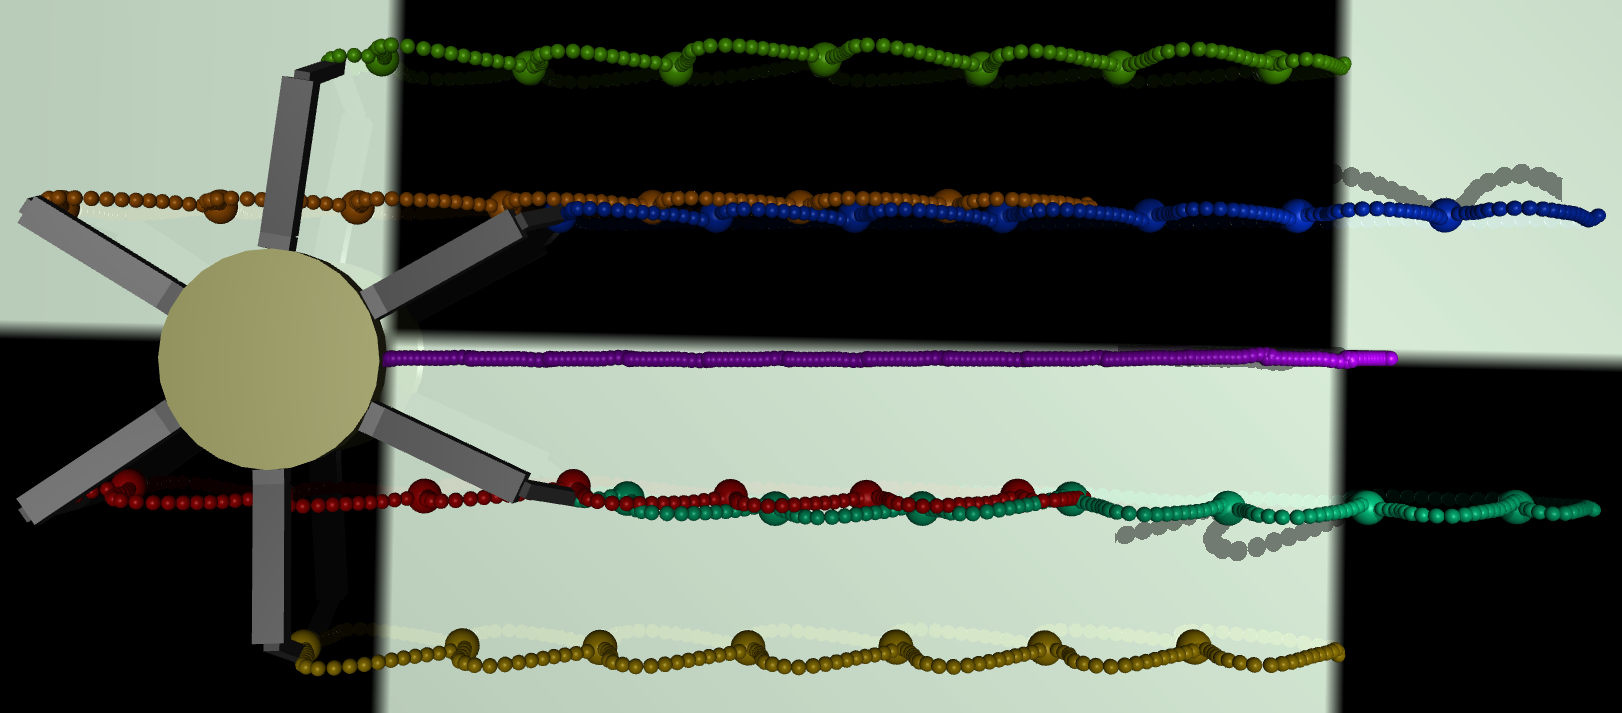
\includegraphics[width=\textwidth]{FlatTop.png}
        \caption{Flat terrain \ac{mujoco} top view.}
        \label{fig:plane_test_top}
    \end{figure}
    
    \noindent
    The simulation results for the body feet trajectories are show in Figure \ref{fig:flat_feet},
    \begin{figure}[h]
        \centering
        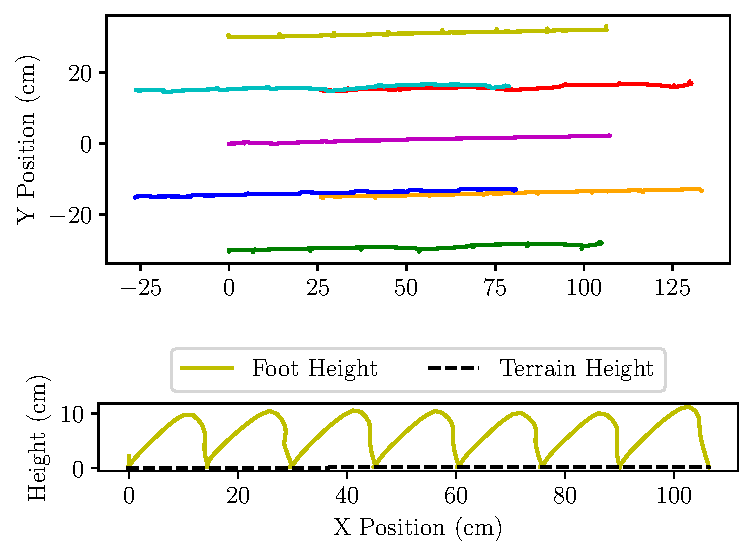
\includegraphics{flat_test_feet.pdf}
        \caption{Flat terrain. Feet top view (Top). One foot side view (Bottom).}
        \label{fig:flat_feet}
    \end{figure}

    \noindent
    where the color codes match that of the above screenshots. It can be seen that the stride length is equal to the set stride of \(15cm\). The robot also maintains a linear trajectory throughout the test. Note that the step height is about \(10cm\) which is a little lower than expected. The reason for this is that the swinging feet are being "pushed" through the flow function faster by the supporting legs faster than expected. Thus, resulting in a lower arc.

    Figure \ref{fig:flat_body} shows the body height and rotation. Here it can be seen that there is a constant error of about 1cm in the body height of the robot. The reason for this is that there is no body height feedback control, as such, errors in the servos accumulate to result in the body height error. This can be easily solved by adding a constant offset or by adding feedback control for the body height.
    \begin{figure}[h]
        \centering
        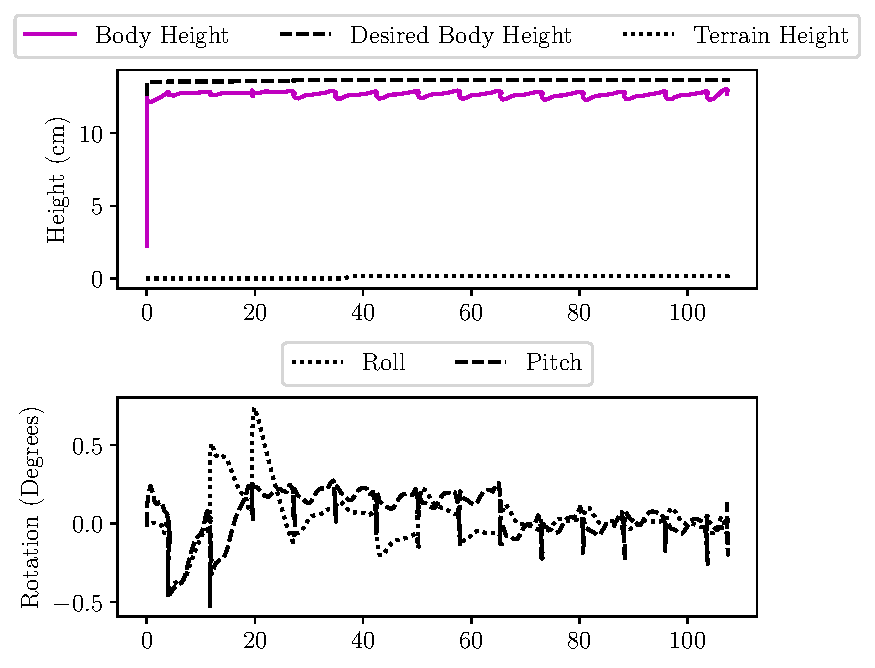
\includegraphics{flat_test_body.pdf}
        \caption{Flat terrain. Body height (Top). Body tilt (Bottom).}
        \label{fig:flat_body}
    \end{figure}
    It is also clear that as the robot walks there are some oscillations in the body height. This is to be expected as the servos are not modeled as having infinite torque, thus, the robot will sag when three legs are lifted off the ground, and rebound once those legs are placed on the floor again. Similarly to the body height error, adding feedback control on the body height would reduce these oscillations. The amplitude of the oscillations are lower than the \(10\%\) of the desired body height, which is acceptable. Next, it can be seen that the tilt of the body also exhibit small oscillations, in both roll and pitch. However, the amplitudes of these oscillations remain below 0.5 degrees.

    
    \section{Staircase}
    A staircase test was performed where the hexapod was commanded to move onto a set of steps. This tested the system's ability to choose foot placements that are not close to edges, to maintain a level body, and to automatically adjust its body height relative to the local terrain height. Figure \ref{fig:stairs} show screenshots of the test simulation in \ac{mujoco}. A video of the simulation can be found \href{https://youtu.be/6v_fmXEp1Vs}{\underline{here}}.
    \begin{figure}[h]
        \centering
        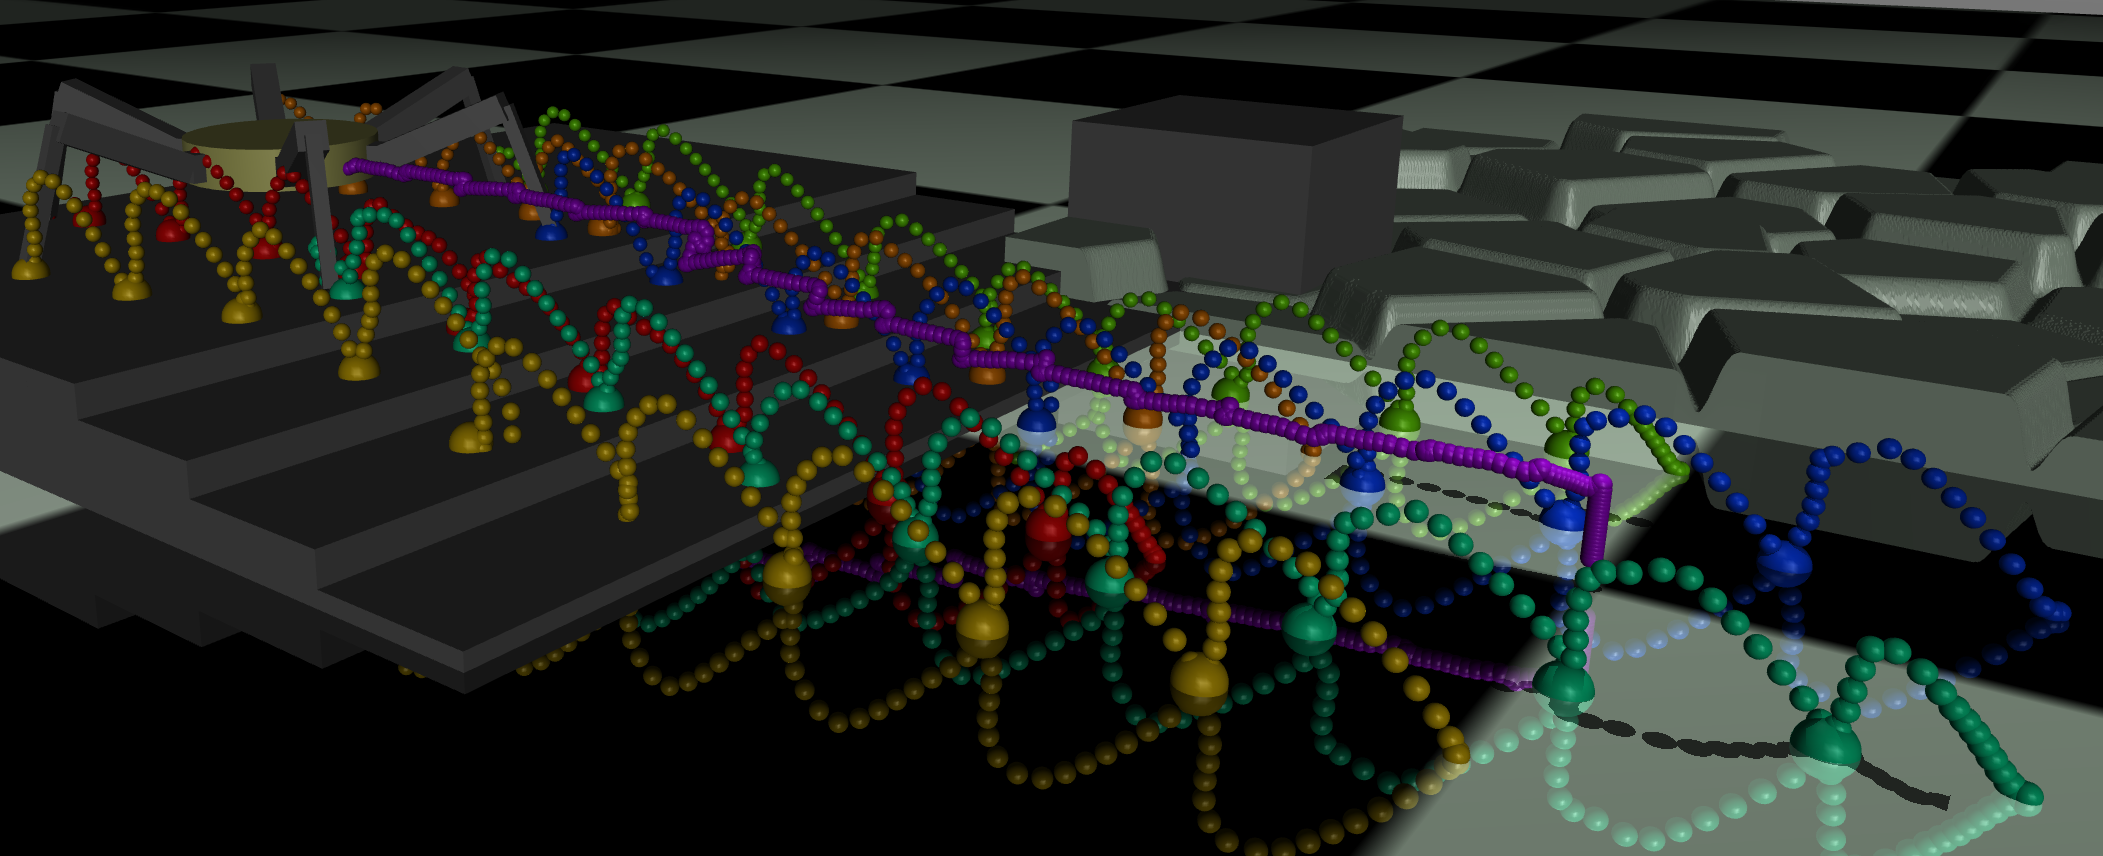
\includegraphics[width=\textwidth]{Stairs.png}
        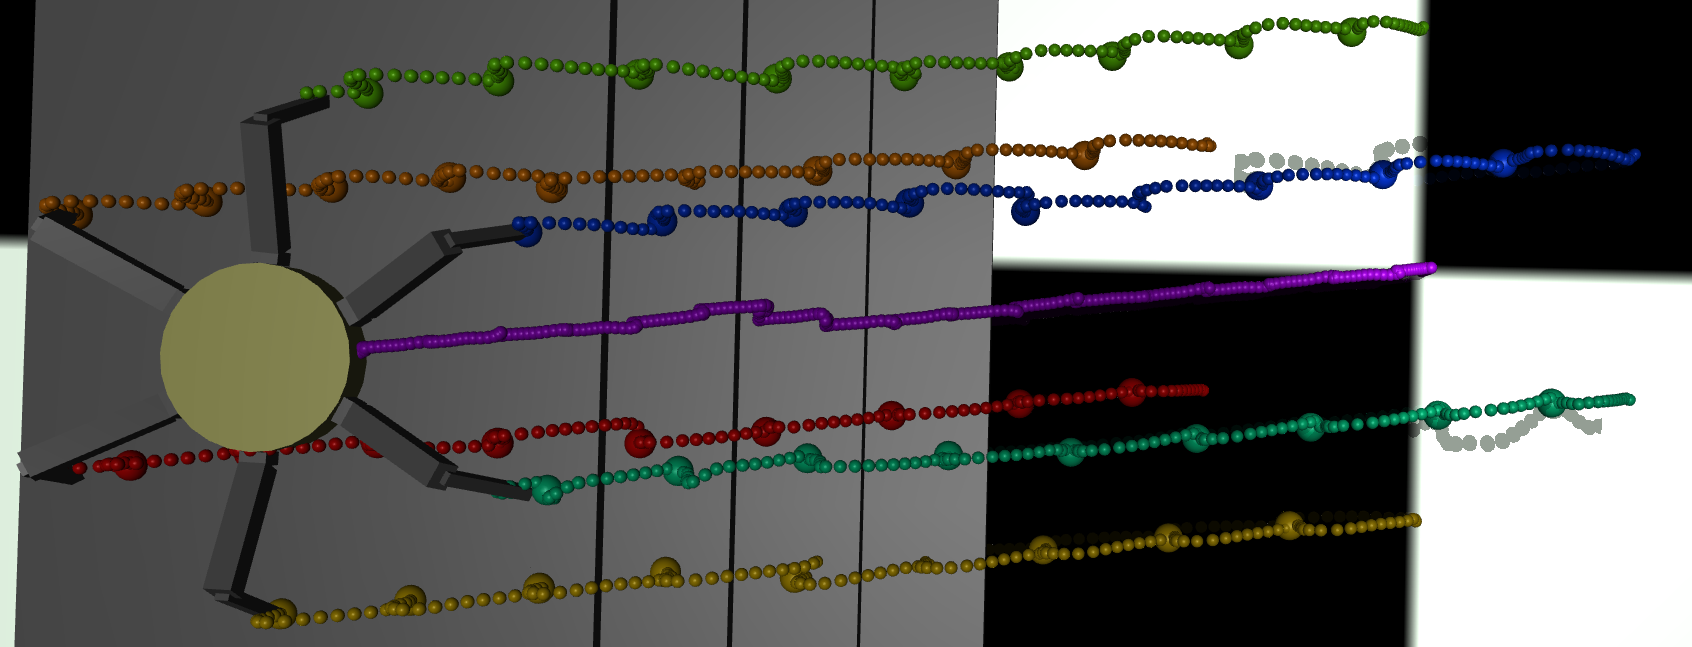
\includegraphics[width=\textwidth]{StairsTop.png}
        \caption{Stairs \ac{mujoco} view.}
        \label{fig:stairs}
    \end{figure}

    \noindent
    The test was performed with a nominal \(15cm\) stride length, the flow parameters \(Ch\) and \(q\) were set to \(2.0\) and \(14.0\) respectively. This results in a step height roughly equal to the true stride length. The target body height is set to \(9cm\) target height above the virtual floor height (see section \ref{sec:height_adjust}). The robot was commanded to walk forwards at a constant velocity.

    % \begin{figure}[h]
    %     \centering
    %     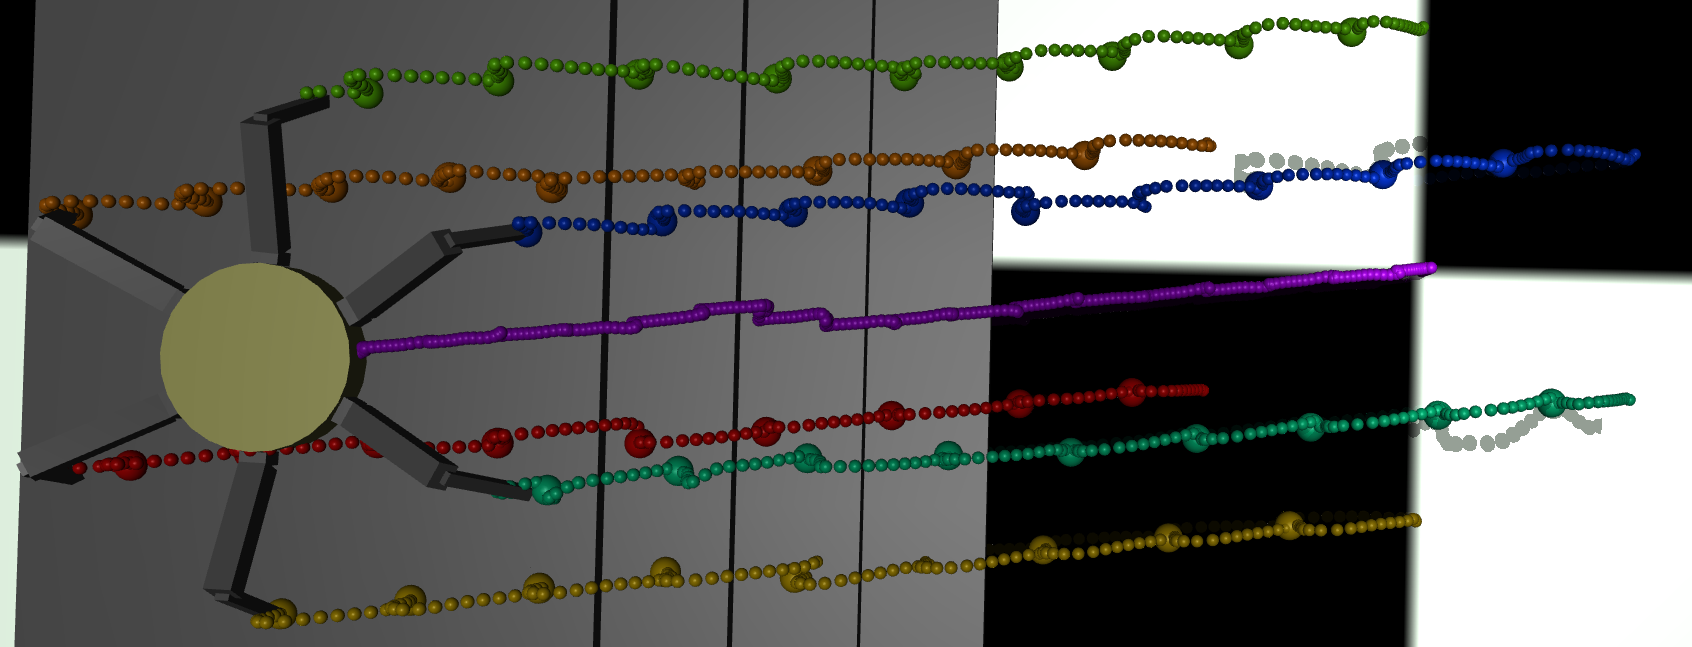
\includegraphics[width=.9\textwidth]{StairsTop.png}
    %     \caption{Stairs \ac{mujoco} view top}
    %     \label{fig:stairs_top}
    % \end{figure}
    The body and feet trajectories are show in figure \ref{fig:stairs_feet}. The robot maintains a mostly linear trajectory up the staris, with a small deviation around \(80cm\) down the X axis. The stride lenght is mostly equal to the nominal \(15cm\), however, the step starting at \(70cm\) has a visibly longer stride length, this is to avoid stepping on the edge of the step. Also note that some steps start with a small loop, this occurs when the robot bumps itself backwards with the front feet. This happens when the front feet push into the ground during a longer stride, due to the slight error in the body height. Similarly to the flat terrain test, the constant body height error is still present. 
    \begin{figure}[h]
        \centering
        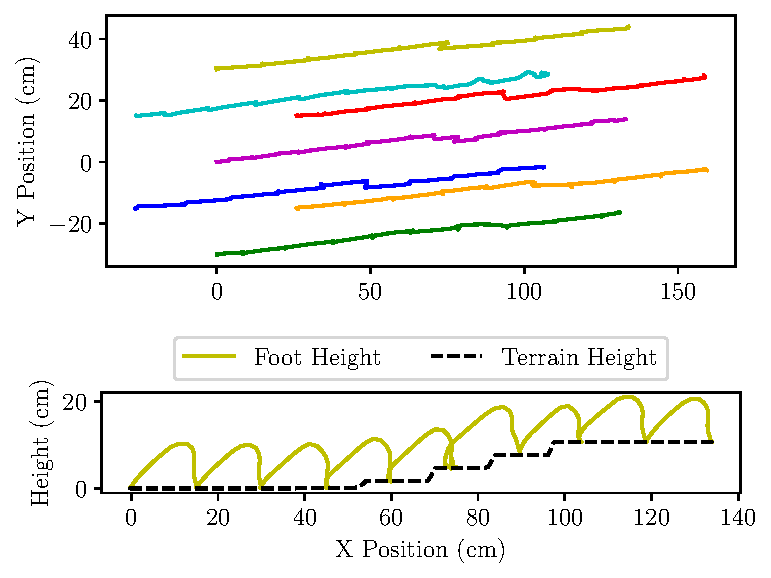
\includegraphics{stairs2_test_feet.pdf}
        \caption{Stairs. Feet top view (Top). One foot side view (Bottom).}
        \label{fig:stairs_feet}
    \end{figure}

    \noindent
    Figure \ref{fig:stairs_body} shows the body height and rotation. From this it can be seen that the robot does increase its height to maintain a constant height above the terrain. It is clear that the body height is not increased in the four discrete steps as the stairs do, rather the body height is increased more smoothly using many smaller steps. This is thanks to the system described in section \ref{sec:height_adjust}.
    The oscillations in the body tilt angles are more prominent in the staircase test than in the flat terrain test, but still mostly stay below 1 degrees, with some intermittent jumps approaching 2 degrees.
    \begin{figure}[h]
        \centering
        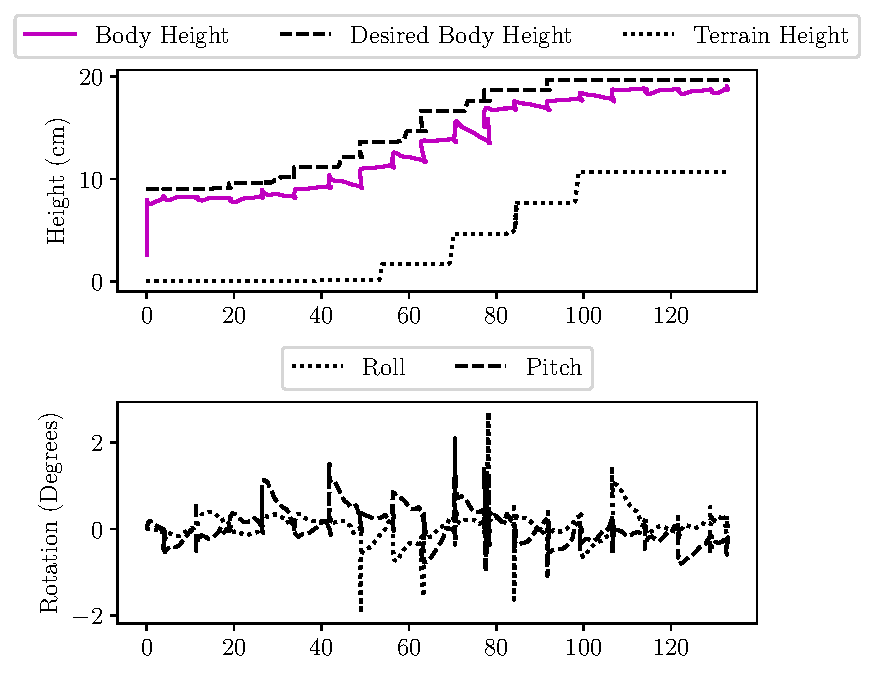
\includegraphics{stairs2_test_body.pdf}
        \caption{Stairs. Feet top view (Top). One foot side view (Bottom).}
        \label{fig:stairs_body}
    \end{figure}

    \section{Cobblestone terrain}
    An organic terrain test was performed where the hexapod was commanded to move over uneven terrain consisting of "cobblestones" with grooves between them and with varying slopes and heights. Figure \ref{fig:org_test} and \ref{fig:org_test_top} show screenshots
    \begin{center}
        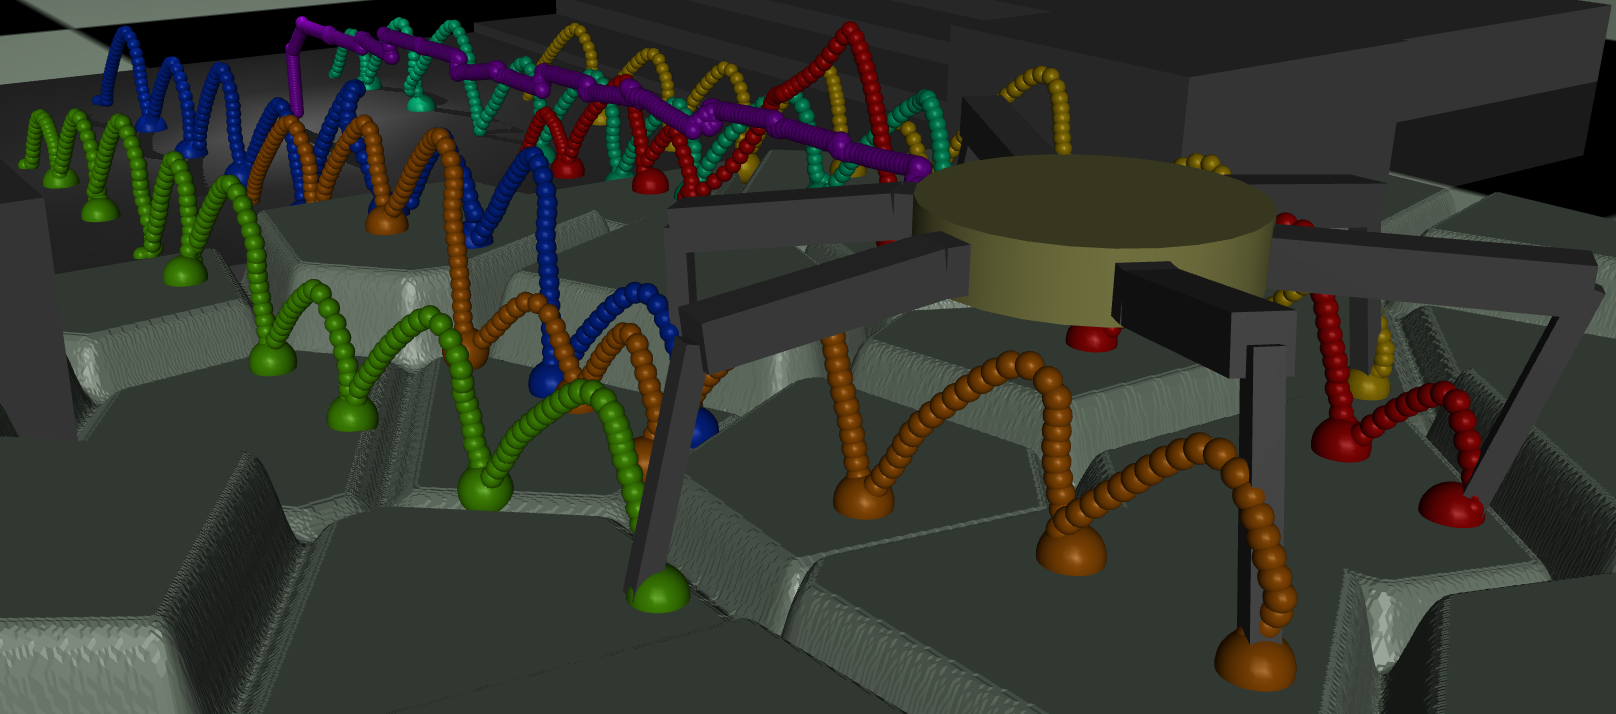
\includegraphics[width=.83\textwidth]{Cobble.png}
        \captionof{figure}{Cobblestone test \ac{mujoco} view.}
        \label{fig:org_test}
    \end{center}
    of the cobblestone test in \ac{mujoco}. A video of the simulated test can be seen \href{https://youtu.be/-lQjvykGlmY}{\underline{here}}. The cobblestones presented islands of suitable foot placement locations, while the grooves represented areas that are not suitable for foot placement. This tested the system's ability to choose suitable foot placements, to maintain a level body and a desired body height, and to traverse uneven terrain.
    % \captionsetup[figure]{oneside,margin={0.9cm,0cm}}
    \begin{figure}[h]
        \centering
        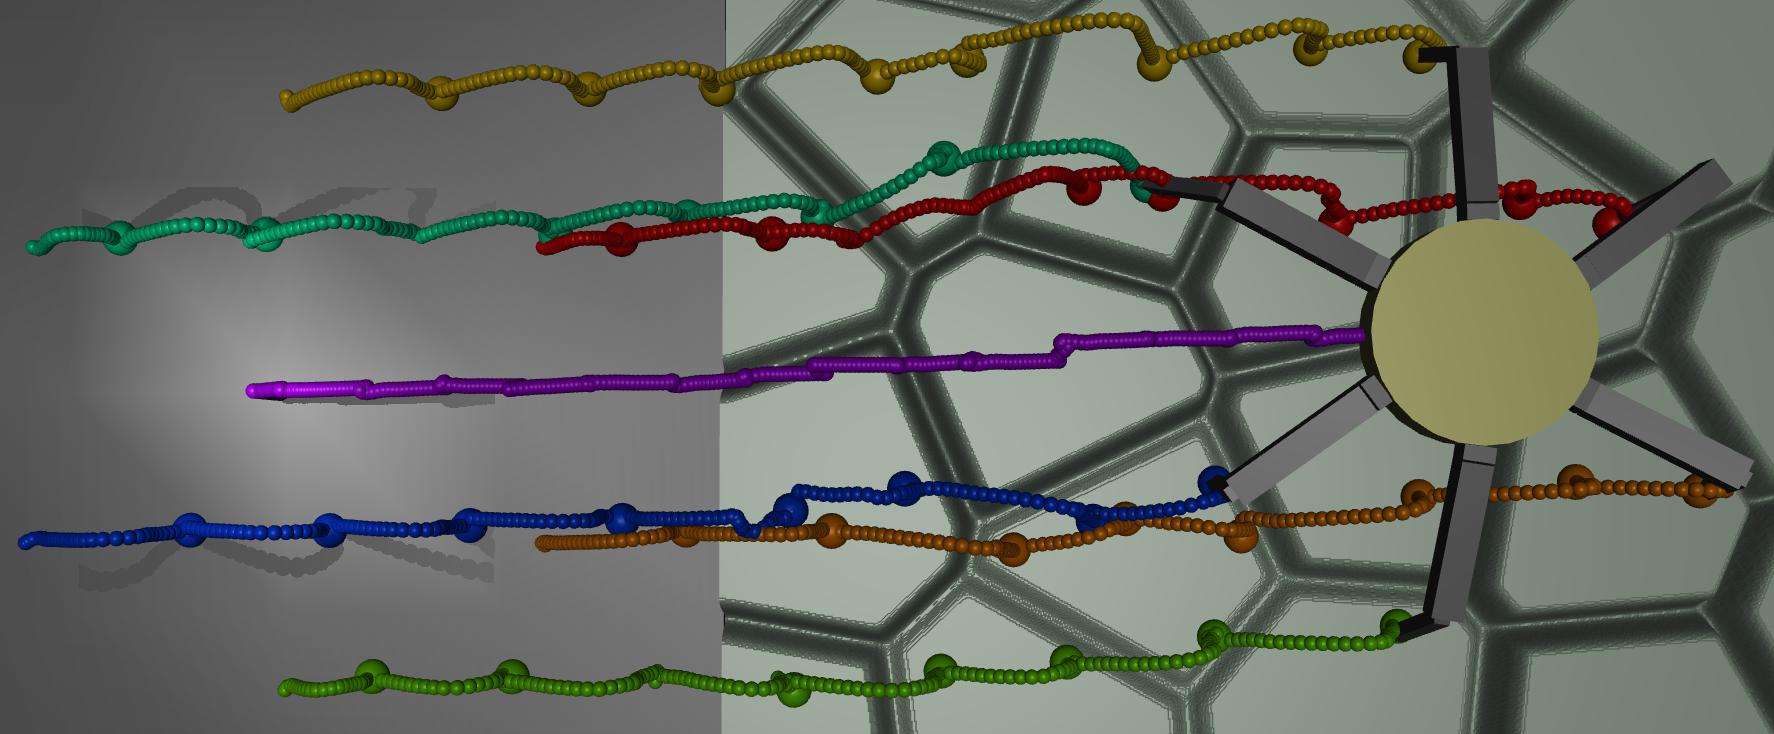
\includegraphics[width=.83\textwidth]{CobbleTop.png}
        \caption{Cobblestone test \ac{mujoco} top view.}
        \label{fig:org_test_top}
    \end{figure}

    \noindent
    Similar to past tests, the robot was commanded to walk over the terrain in a straight line at a constant velocity. The nominal stride length was set to \(15cm\) and the flow parameters \(Ch\) and \(q\) were set to \(2.0\) and \(14.0\) respectively. Figure \ref{fig:cobble_feet} shows the body and leg trajectories. The robot still maintains a straight

    \begin{centering}
        \centering
        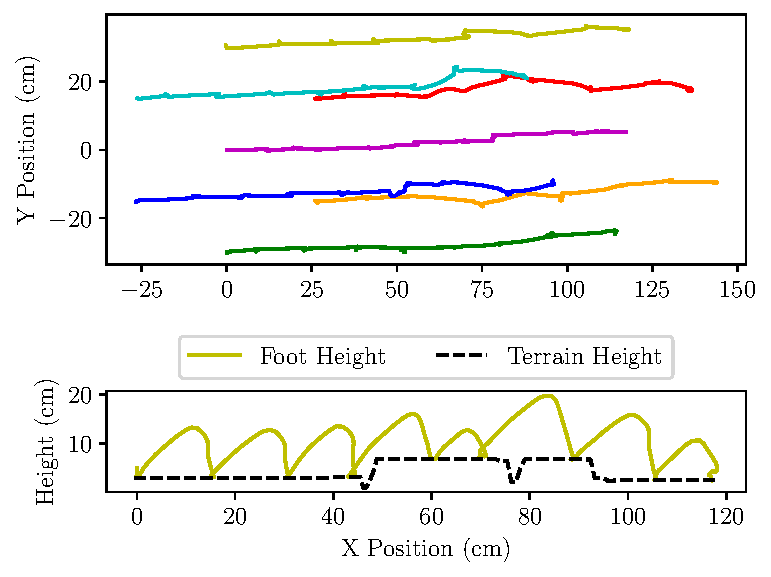
\includegraphics{cobble_test_feet.pdf}
        \captionof{figure}{Cobblestones. Feet top view (Top). One foot side view (Bottom).}
        \label{fig:cobble_feet}
    \end{centering}
    \noindent
    trajectory over the terrain. This test clearly demonstrates how the robot adjusts its feet targets in the horizontal plane to place them on the cobbles. Similarly, stride length is also greatly adjusted, as can be seen from figure \ref{fig:cobble_feet}.

    Figure \ref{fig:cobble_body} shows the body heigh and rotation during the cobblestone terrain test.
    \begin{figure}[h]
        \centering
        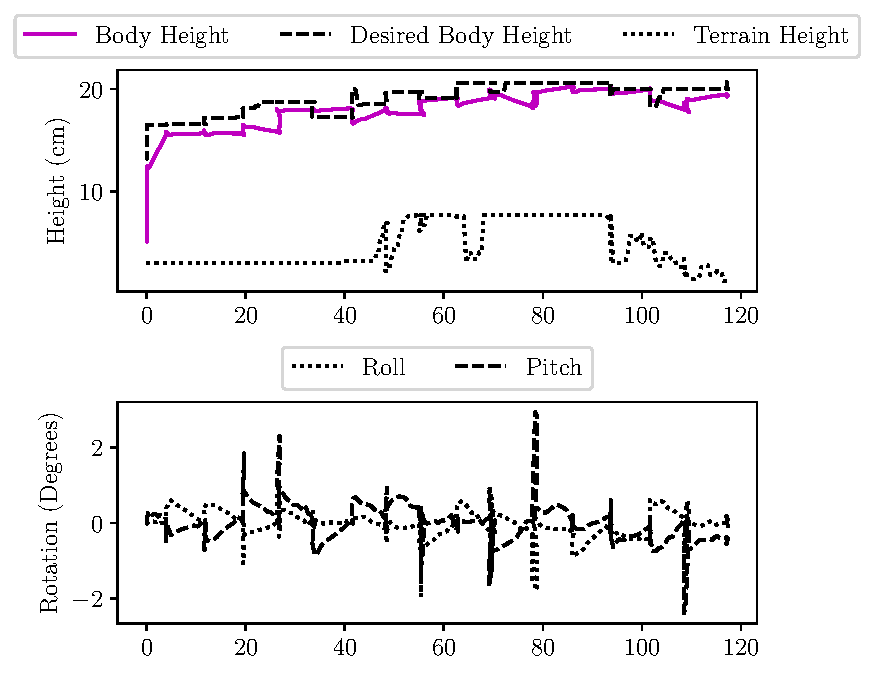
\includegraphics{cobble_test_body.pdf}
        \caption{Cobblestones. Body height (Top). Body tilt (Bottom).}
        \label{fig:cobble_body}
    \end{figure}
    From this it can be seen that the body height error seen in the flat plane test is still present, and more severe. However, the body height still stays within a reasonable margin from the desired height.

    For the most part, the oscillations in the body rotation is similar to that of the stairs test. However, they are more frequent, and more sever spikes are present. This is due, in part, to the more erratic mismatch between the body height and the requested body height. The horizontal adjustments made to the foot placement positions cause the swinging feet to end their steps at different times. This is the primary cause of the tilt spikes, as when one foot is placed on the floor before the other two, the robot is tilted slightly. This, however, would not occur if there was no, or little, error in the body height control.

    % Finally, when looking at the foot position plot in figure \ref{fig:org_test_data}, please note that the plot is a projection into the X-Z plane, and thus any adjustment made in the Y-axis is not shown, the foot shown has been chosen to include minimum Y-axis variation. Thus, please also see the 3D view in figure \ref{fig:org_test}. From these two figures it is clear that the foot end positions are, in addition to height, adjusted in the horizontal plane, the step arcs are appropriately adjusted and remain relatively smooth, similar to the flat plane test.


% \bigskip
% \bigskip
% \hrule
% \smallbreak
% \hrule


\chapter{Conclusions}


\appendix%------------------------------------------------------------
\chapter{Mathematical proofs}

\section{Euler's equation}
Euler's equation gives the relationship between the trigonometric functions and the complex exponential function.
\begin{equation}
    e^{ i\theta } = \cos \theta + i\sin \theta
    \label{eq:Euler}
\end{equation}
Inserting $\theta=\pi$ in \eqref{eq:Euler} results in Euler's identity
\begin{equation}
    e^{ i \pi} + 1 = 0
    \label{eq:Euler2}
\end{equation}


\section{Navier Stokes equation}

The Navier–Stokes equations mathematically express momentum balance and conservation of mass for Newtonian fluids.  Navier-Stokes equations using tensor notation:
\begin{subequations}
\begin{gather}
    \frac{\partial \rho}{\partial t} +
    \frac{\partial}{\partial x_j}\left[ \rho u_j \right] = 0 
    \\
    \frac{\partial}{\partial t}\left( \rho u_i \right) +
    \frac{\partial}{\partial x_j}
    \left[ \rho u_i u_j + p \delta_{ij} - \tau_{ji} \right] = 0, \quad i=1,2,3
    \\
    \frac{\partial}{\partial t}\left( \rho e_0 \right) +
    \frac{\partial}{\partial x_j}
    \left[ \rho u_j e_0 + u_j p + q_j - u_i \tau_{ij} \right] = 0
\end{gather}
\end{subequations}

\chapter{Experimental results}


\backmatter%----------------------------------------------------------
\bibliography{bib/bib-sample}
 
\end{document}   

